% Dharma technical manual.
% Build: make -C docs manual  (output: docs/build/manual/dharma_manual.pdf)
\documentclass[11pt,a4paper,oneside]{report}

\usepackage[T1]{fontenc}
\usepackage[utf8]{inputenc}
\usepackage{mathptmx}
\usepackage[scaled=0.92]{helvet}
\usepackage{courier}
\usepackage[margin=2.3cm,headheight=14pt]{geometry}
\usepackage{amsmath,amssymb}
\usepackage{graphicx}
\usepackage{booktabs,longtable,tabularx,array}
\usepackage{xcolor}
\usepackage{enumitem}
\usepackage{pdflscape}
\usepackage{caption}
\usepackage{fancyhdr}
\usepackage{titlesec}
\usepackage{listings}
\usepackage[hyphens]{url}
\usepackage[hidelinks]{hyperref}
\usepackage{cite}

% Author and affiliations of every Dharma document (paper and manual). Change them here only.
\newcommand{\DharmaAuthor}{I Wayan Agus Darmawan}
\newcommand{\DharmaEmail}{darmawandeveloper@gmail.com}
\newcommand{\DharmaAffilOne}{Department of Computer Engineering, Institut Teknologi Sepuluh
  Nopember (ITS), Surabaya, Indonesia}
\newcommand{\DharmaAffilTwo}{PT Ezra Robotics Teknologi, Indonesia}
\newcommand{\DharmaVersion}{0.2.0}

% Macros shared by the paper and the manual (needs xcolor and amsmath).

% Placeholder for content that phase 2 fills in (measured results, test names). Renders in red
% so nothing unfinished goes unnoticed.
\newcommand{\todo}[1]{\textcolor{red}{\textbf{[TODO:} #1\textbf{]}}}
% A number still to be measured, for tables.
\newcommand{\tbd}{\textcolor{red}{\textbf{??}}}

% Names
\newcommand{\pkg}[1]{\texttt{#1}}
\newcommand{\topic}[1]{\texttt{#1}}
\newcommand{\frm}[1]{\texttt{#1}}
\newcommand{\param}[1]{\texttt{#1}}

% Math
% {}^{a}T_{b}: pose of frame b in frame a (maps points from b to a), the TF edge a -> b.
\newcommand{\T}[2]{{}^{#1}\mathbf{T}_{#2}}
\newcommand{\R}{\mathbb{R}}
\newcommand{\SE}[1]{\mathrm{SE}(#1)}
\newcommand{\vect}[1]{\boldsymbol{#1}}
\newcommand{\tr}{t_{\mathrm{r}}}
\newcommand{\amax}{a_{\mathrm{dec}}}


\graphicspath{{../diagrams/pdf/}}

% Identifiers (topics, parameters, packages) with raw underscores, breakable at / _ . -
\makeatletter
\g@addto@macro\UrlBreaks{\do\_\do\.\do\-}
\makeatother
\newcommand{\code}[1]{\nolinkurl{#1}}
\renewcommand{\pkg}[1]{\code{#1}}
\renewcommand{\topic}[1]{\code{#1}}
\renewcommand{\frm}[1]{\code{#1}}
\renewcommand{\param}[1]{\code{#1}}

\titleformat{\chapter}[display]{\sffamily\bfseries\huge}{\large\chaptertitlename\
  \thechapter}{8pt}{}
\titleformat{\section}{\sffamily\bfseries\Large}{\thesection}{0.6em}{}
\titleformat{\subsection}{\sffamily\bfseries\large}{\thesubsection}{0.6em}{}
\titleformat{\subsubsection}{\sffamily\bfseries}{\thesubsubsection}{0.6em}{}
\titlespacing*{\chapter}{0pt}{0pt}{18pt}

\pagestyle{fancy}
\fancyhf{}
\fancyhead[L]{\sffamily\small Dharma \DharmaVersion\ technical manual}
\fancyhead[R]{\sffamily\small\nouppercase{\leftmark}}
\fancyfoot[C]{\sffamily\small\thepage}
\renewcommand{\headrulewidth}{0.4pt}

\setlist{itemsep=2pt,topsep=4pt}
\setlength{\parskip}{4pt}
\setlength{\parindent}{0pt}
\setlength{\emergencystretch}{3em}
\renewcommand{\arraystretch}{1.15}
\captionsetup{font=small,labelfont=bf}

\lstset{basicstyle=\ttfamily\small,columns=fullflexible,keepspaces=true,breaklines=true,
  showstringspaces=false,
  frame=single,rulecolor=\color{black!30},backgroundcolor=\color{black!3},
  xleftmargin=4pt,xrightmargin=4pt,aboveskip=6pt,belowskip=6pt}

% "Read-only at runtime" marker of the generated parameter tables
\newcommand{\readonlynote}{Parameters marked $^\dagger$ are read-only at runtime
  (\code{live=False}); every other one can be changed with \texttt{ros2 param set} and is
  validated before it applies.}

\begin{document}

\begin{titlepage}
  \centering
  \vspace*{3cm}
  {\sffamily\bfseries\Huge Dharma\par}
  \vspace{0.6cm}
  {\sffamily\Large A robot-agnostic ROS~2 autonomy stack\par}
  \vspace{0.3cm}
  {\sffamily\large Technical manual, version \DharmaVersion\par}
  \vspace{2.5cm}
  {\large \DharmaAuthor\par}
  \vspace{0.3cm}
  {\small \DharmaAffilOne\\ \DharmaAffilTwo\\ \DharmaEmail\par}
  \vfill
  {\small Architecture, models, configuration, interfaces, the safety case and the development
  guide of the 0.2.0 stack.\par}
\end{titlepage}

\tableofcontents

\chapter{Introduction}
\label{ch:intro}

Dharma is a robot-agnostic autonomy stack for legged and wheeled service robots on ROS~2
Foxy, Humble and Jazzy. It provides LiDAR-inertial odometry with a start gate and a monitor,
fiducial-anchored localization with an extended Kalman filter, occupancy mapping and sites,
route teaching, path planning and following with avoidance around people, a control
multiplexer with a protective field and a latched e-stop, health monitoring, RViz panels and a
simulator. It contains no product features: points of interest, tours, narration and visitor
tracking belong to products built on it (for example the Molly tour-guide robot).

This manual describes version \DharmaVersion. It is written for three readers:
\begin{itemize}
  \item \textbf{integrators} who bring Dharma up on a new robot: Chapters~\ref{ch:arch}
    and~\ref{ch:config} (architecture, robot profile and parameters), Chapter~\ref{ch:control}
    (the safety case) and the interfaces reference (Chapter~\ref{ch:interfaces});
  \item \textbf{developers} who change or extend a package: the subsystem chapters
    (\ref{ch:odometry}--\ref{ch:sim}) with their models and parameters, and
    Chapter~\ref{ch:dev} (layout, style, tests, CI, releases);
  \item \textbf{reviewers} who check that known defects are fixed: Appendix~\ref{app:trace}
    maps every review finding to its fix and its regression test.
\end{itemize}

\section{What changed in 0.2.0}

Version 0.2.0 is a breaking clean-up of the 0.1 stack split out of a product. Two reviews
modelled every subsystem and listed defects with priorities (P0 safety, P1 robustness, P2
maintainability). The main changes:
\begin{itemize}
  \item \textbf{General only.} Points of interest, tours, narration, gestures, visitor tracking
    and the mission status were removed; goals are poses, sites hold a map, fiducials and
    routes.
  \item \textbf{One robot description.} Footprint, base height, kinematics, limits and frames
    come from the shared \param{robot.*} parameters (\code{RobotProfile}); no package declares
    its own geometry.
  \item \textbf{Structure.} Every package has a pure \code{core/} (no ROS imports), a
    \code{utils/} with conversions and thin nodes on \code{DharmaNode}; modules have at most
    300 lines; families of algorithms are plugins.
  \item \textbf{Typed interfaces.} Status topics are typed messages with enum constants;
    safety actions are separate trigger services.
  \item \textbf{Safety.} One braking model for every speed limit; the protective field covers
    rotation and combined motion; blind or stale sensing is an obstacle; the e-stop latches
    reasons, has a hardware input and requires a re-arm; navigation never publishes the
    robot's \topic{cmd_vel}.
  \item \textbf{Estimation.} Gravity-aligned odometry, an EKF over \frm{map}$\to$\frm{odom} with
    covariance and chi-square gating, optional scan matching, mapping with jump and correction
    gates.
\end{itemize}

\section{Conventions of this manual}

Frames, topics, services and parameters are set in \code{typewriter}. Topic names are
relative: a product namespaces the robot driver (\code{/<ns>/cmd_vel}). Units are SI; angles
are radians internally and degrees only in human-facing configuration (parameter names end in
\code{_deg}). A transform $\T{a}{b}$ is the pose of frame $b$ in frame $a$, i.e.\ the TF edge
$a \to b$; it maps points from $b$ to $a$. This edition describes the 0.2.0 code of every
repository; the parameter and interface tables are generated from it
(\code{docs/manual/tools/reference.py}). Measured results are reported in the paper, not here.

\section{Repositories}

\begin{figure}[h]
  \centering
  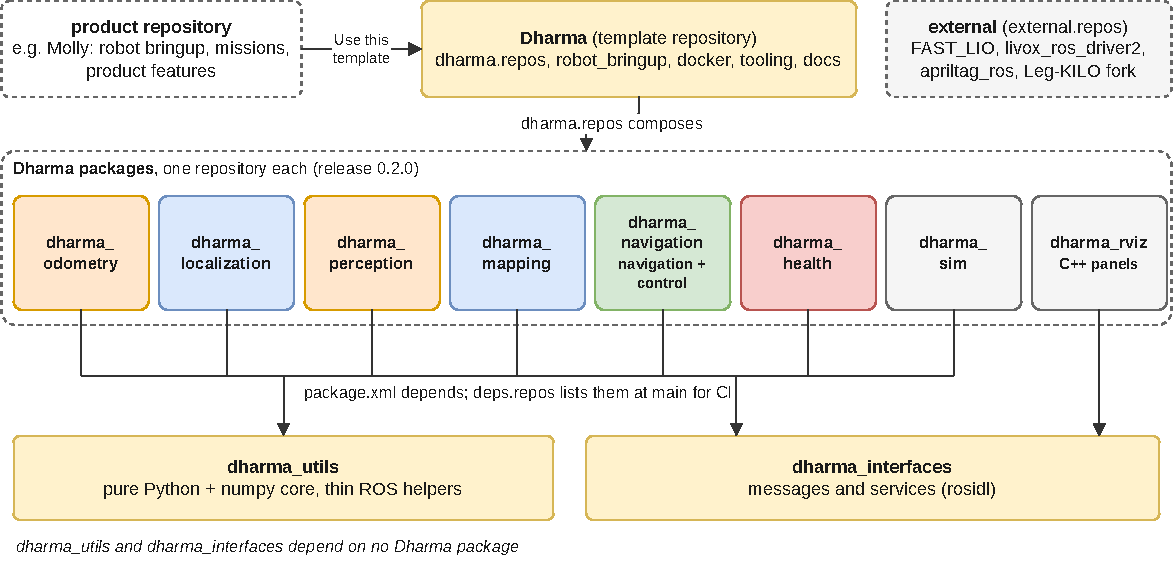
\includegraphics[width=\textwidth]{repos}
  \caption{Repositories and their dependencies. Every package depends only on
    \pkg{dharma_utils} and \pkg{dharma_interfaces}; the Dharma template repository composes
    them, and a product is generated from the template.}
  \label{fig:repos}
\end{figure}

\begin{tabularx}{\textwidth}{@{}lX@{}}
  \toprule
  Repository & Content \\
  \midrule
  \pkg{dharma_utils} & math, typed configuration, robot profile, braking model, io, grid, plugins,
    logging, ROS node helpers, test helpers \\
  \pkg{dharma_interfaces} & messages and services \\
  \pkg{dharma_odometry} & estimator launch (FAST-LIO2, Leg-KILO or external), start gate, monitor \\
  \pkg{dharma_localization} & bridge, EKF over \frm{map}$\to$\frm{odom}, fiducial tags \\
  \pkg{dharma_perception} & sector and safety scans from the LiDAR, camera throttle for fiducials \\
  \pkg{dharma_mapping} & occupancy grid, sites, route recorder \\
  \pkg{dharma_navigation} & packages \pkg{dharma_navigation} (planner, loader, follower,
    avoidance) and \pkg{dharma_control} (control mux) \\
  \pkg{dharma_health} & health monitor and diagnostics \\
  \pkg{dharma_rviz} & RViz panels (C++) \\
  \pkg{dharma_sim} & simulator with drift, latency and dropout \\
  \code{Dharma} & template repository: workspace, docker, bringup skeleton, tooling, documentation \\
  \bottomrule
\end{tabularx}

\chapter{Architecture}
\label{ch:arch}

\section{Layers}

\begin{figure}[h]
  \centering
  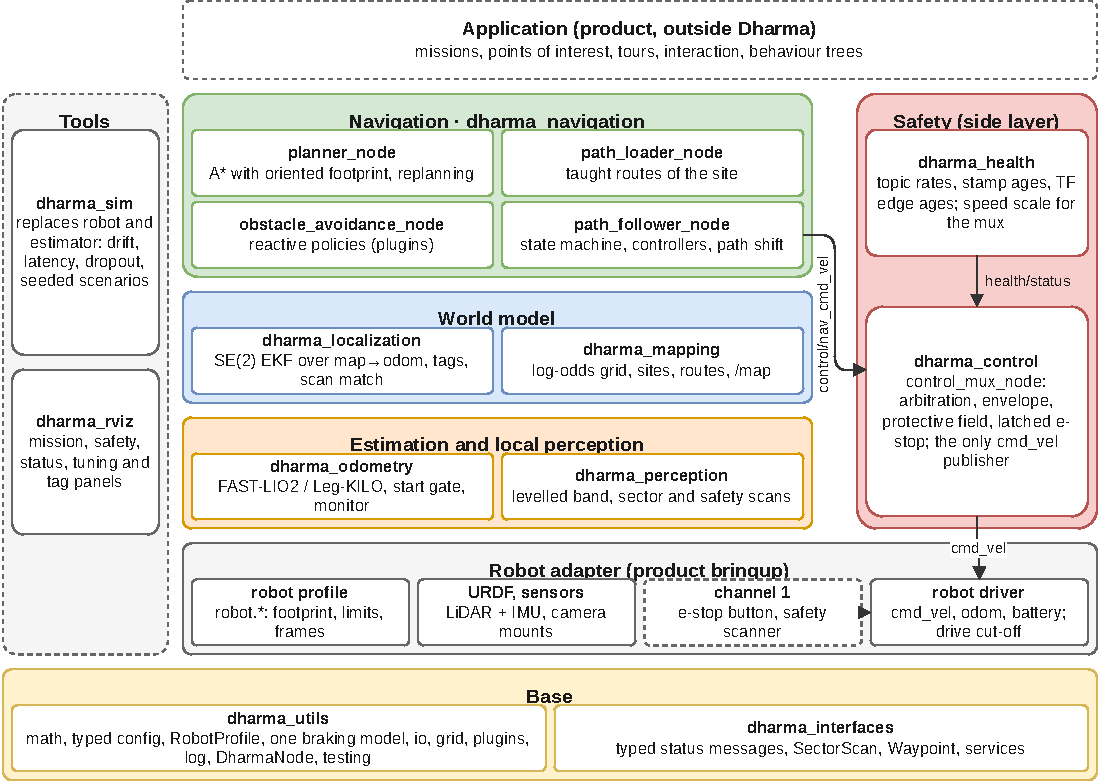
\includegraphics[width=\textwidth]{layers}
  \caption{Layers of Dharma. Colours: estimation orange, world model blue, navigation green,
    safety red, base yellow, hardware grey.}
  \label{fig:layers}
\end{figure}

Dharma is organised in layers (Fig.~\ref{fig:layers}); each depends only on the layers below and
on the base packages.

\begin{description}
  \item[Robot adapter] (product). The driver bridge (velocity command in, robot odometry and
    battery out), the URDF with the sensor mounts, and the robot profile. A hardware e-stop and,
    where required, a safety-rated scanner act on the drive directly (channel~1,
    Section~\ref{sec:two-channel}).
  \item[Estimation and local perception.] \pkg{dharma_odometry} runs a LiDAR-inertial estimator
    and monitors it; \pkg{dharma_perception} turns the LiDAR into obstacle sectors around the
    robot and throttles the camera for the fiducial detector.
  \item[World model.] \pkg{dharma_localization} keeps \frm{map}$\to$\frm{odom} from fiducials,
    operator input and optional scan matching; \pkg{dharma_mapping} records occupancy maps and
    manages sites and routes.
  \item[Navigation.] \pkg{dharma_navigation} plans on the map, loads taught routes, follows
    paths and runs reactive avoidance. Its velocity output is \topic{control/nav_cmd_vel},
    never the robot's \topic{cmd_vel}.
  \item[Safety] (side layer). \pkg{dharma_control} is the only publisher of \topic{cmd_vel}: it
    arbitrates navigation and operators, applies the envelope and the protective field and
    latches the e-stop. \pkg{dharma_health} watches rates, ages and system resources and
    requests a speed scale from the mux.
  \item[Base.] \pkg{dharma_utils} and \pkg{dharma_interfaces}.
  \item[Tools.] \pkg{dharma_sim} replaces the robot and the estimator in simulation;
    \pkg{dharma_rviz} provides operator panels.
\end{description}

\section{Data flow}

Fig.~\ref{fig:dataflow} shows the nodes and the main topics between them; the interfaces
reference (Chapter~\ref{ch:interfaces}) lists every message and service.

\begin{landscape}
\begin{figure}
  \centering
  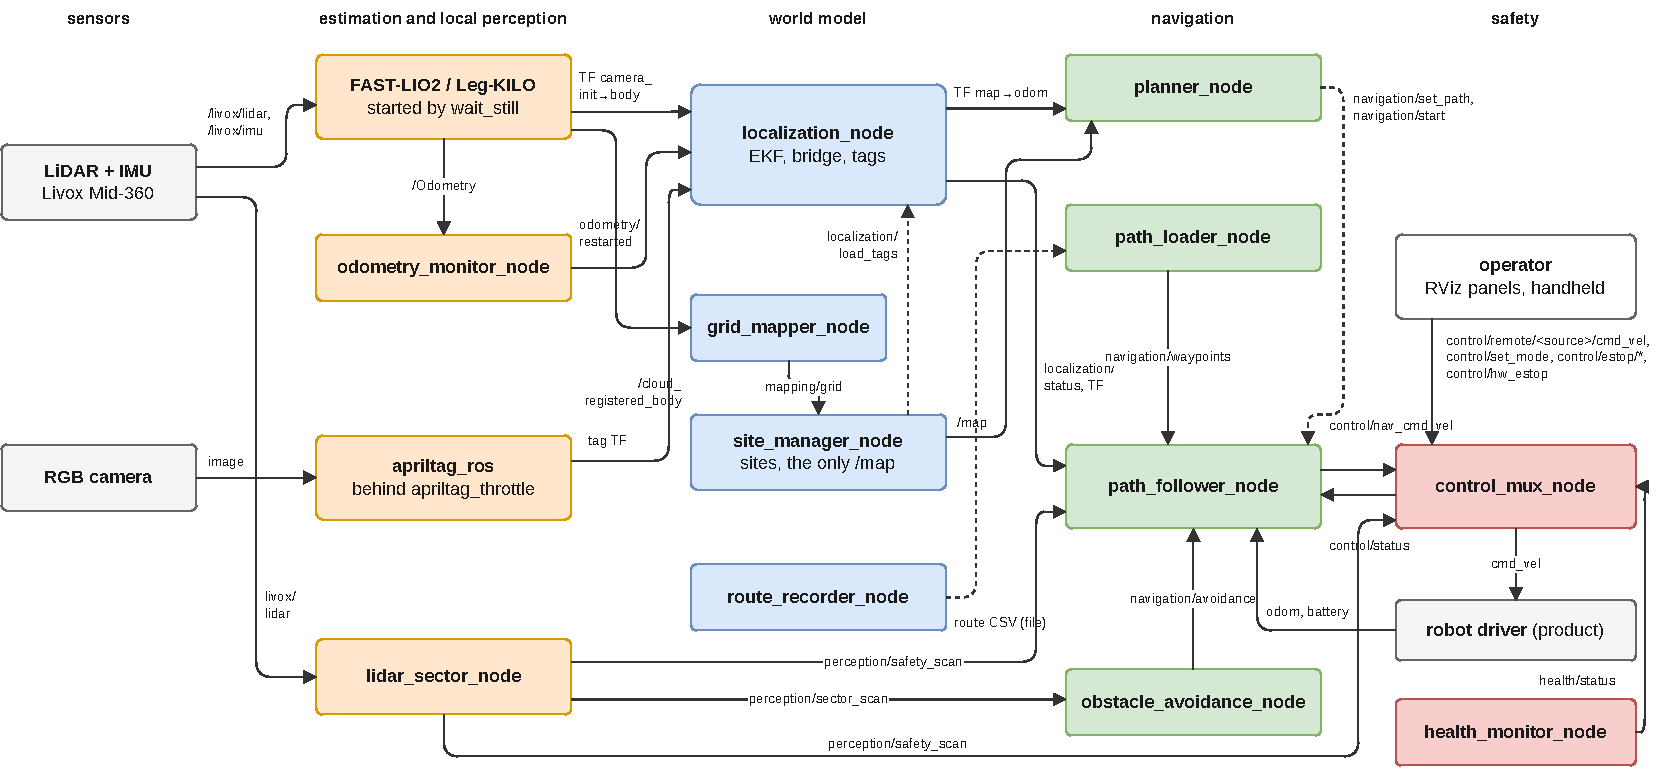
\includegraphics[width=\linewidth]{dataflow}
  \caption{Nodes and main topics. Solid: topics and TF; dashed: services and files.}
  \label{fig:dataflow}
\end{figure}
\end{landscape}

\begin{longtable}{@{}p{0.14\textwidth}p{0.36\textwidth}p{0.20\textwidth}p{0.20\textwidth}@{}}
  \toprule
  Package & Publishes & Subscribes & Services \\
  \midrule
  \endhead
  \bottomrule
  \endfoot
  odometry & \topic{odometry/status} (OdometryStatus, latched), \topic{odometry/restarted}
    (Empty) & \topic{/Odometry}, leg odometry, IMU & -- \\
  localization & TF \frm{map}$\to$\frm{odom} and the bridge (\frm{odom}$\to$\frm{camera_init},
    \frm{body}$\to$\frm{base_link}), \topic{localization/status} (latched),
    \topic{localization/pose} (PoseWithCovarianceStamped), \topic{localization/tag_markers} &
    \topic{odometry/restarted}, \topic{/initialpose}, IMU, \topic{/map} and the registered cloud
    (scan matching) & \topic{localization/start}, \topic{reset}, \topic{assume_origin},
    \topic{record_tags}, \topic{load_tags} \\
  perception & \topic{perception/sector_scan} (front), \topic{perception/safety_scan} (360°),
    \topic{perception/obstacles} & Livox CustomMsg or PointCloud2, TF & -- \\
  mapping & \topic{/map} (latched, only publisher), \topic{mapping/grid},
    \topic{mapping/status}, \topic{site/status}, \topic{route/saved} & registered cloud,
    \topic{localization/status} & \topic{site/list}, \topic{site/load}, \topic{mapping/start},
    \topic{mapping/stop}, \topic{mapping/save}, \topic{route/start}, \topic{route/stop},
    \topic{route/mark_stop_point} \\
  navigation & \topic{planner/path}, \topic{planner/status}, \topic{planner/costmap},
    \topic{navigation/status}, \topic{navigation/stop_point}, \topic{navigation/path},
    \topic{navigation/waypoints}, \topic{navigation/avoidance}, \topic{control/nav_cmd_vel},
    markers & \topic{/map}, \topic{perception/*_scan}, \topic{control/status},
    \topic{localization/status}, battery, odom & \topic{planner/go_to}, \topic{planner/plan},
    \topic{planner/cancel}, \topic{navigation/set_path}, \topic{navigation/load_path},
    \topic{navigation/start}, \topic{stop}, \topic{pause}, \topic{resume} \\
  control & \topic{cmd_vel} (only publisher), \topic{control/status} (latched) &
    \topic{control/nav_cmd_vel}, \topic{control/remote/<source>/cmd_vel},
    \topic{perception/safety_scan}, \topic{control/estop_request}, \topic{control/hw_estop},
    \topic{health/status} & \topic{control/set_mode}, \topic{control/estop/engage},
    \topic{control/estop/release} \\
  health & \topic{health/status} (latched), \topic{diagnostics} & configured topics, status
    topics, TF & -- \\
\end{longtable}

\section{Frames}
\label{sec:frames}

\begin{figure}[h]
  \centering
  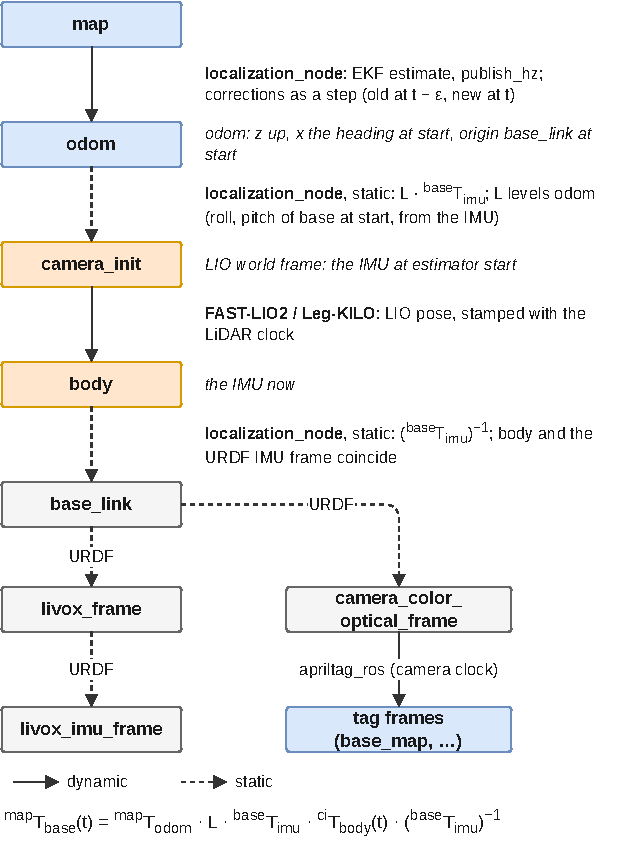
\includegraphics[width=0.62\textwidth]{tf_tree}
  \caption{TF tree and who publishes each edge.}
  \label{fig:tf}
\end{figure}

The tree follows REP-105 (Fig.~\ref{fig:tf}). The LiDAR-inertial estimator publishes
\frm{camera_init}$\to$\frm{body}: \frm{camera_init} is the IMU frame at estimator start and
\frm{body} the IMU now. Localization bridges it into the robot tree with two static transforms
and publishes the map correction:
\begin{equation}
  \T{map}{base}(t) = \T{map}{odom}\; \underbrace{L\, \T{base}{imu}}_{\T{odom}{ci}}\;
  \T{ci}{body}(t)\; \underbrace{\big(\T{base}{imu}\big)^{-1}}_{\T{body}{base}} .
  \label{eq:m-chain}
\end{equation}
$\T{base}{imu}$ is the URDF mounting of the IMU and $L$ the roll and pitch of the base at
estimator start (Section~\ref{sec:leveling}). Consequently \frm{odom} has $z$ against gravity,
its $x$ axis is the heading at start and its origin is \frm{base_link} at start. Frame names
come from \param{robot.frames.*}; the LIO frames are parameters of localization.

The edges with time-varying values are \frm{map}$\to$\frm{odom} (stamped by localization with
the node clock) and \frm{camera_init}$\to$\frm{body} (stamped by the estimator with the LiDAR
clock); everything else is static. This matters for the TF latency budget
(Section~\ref{sec:tf-budget}).

\section{Design principles}

\begin{enumerate}
  \item \textbf{One source of truth for the robot.} Every geometric and dynamic assumption is
    derived from the robot profile (Chapter~\ref{ch:config}); derived values are computed,
    never copied.
  \item \textbf{Pure core, ROS at the edge.} Algorithms are plain Python and numpy, unit-tested
    without ROS; nodes convert messages at the edge.
  \item \textbf{Plugins instead of if/elif.} Controllers and avoidance policies register in a
    named registry, open to entry points.
  \item \textbf{Uncertainty in the interfaces.} The robot pose is published with its
    covariance; statuses carry states, sigmas and reasons.
  \item \textbf{Safety independent of autonomy.} The safety layer only reads typed inputs and
    can be verified on its own; navigation pauses itself on the control status.
  \item \textbf{Fail safe.} Missing data is an obstacle; a failing callback stops the robot.
  \item \textbf{Compatibility.} SemVer; every package of the stack moves together across a
    breaking change.
\end{enumerate}

\section{Launch composition}

Each package has one launch file (\code{launch/<pkg>.launch.py}) with the arguments
\code{params_file}, \code{robot_params}, \code{use_sim_time} and \code{log_level}; parameters
are applied as \texttt{[package defaults, robot\_params, params\_file, non-empty overrides]}, so an
empty argument never overrides a value from a file. No package launch file includes another
one: the product bringup (generated from the template's \code{robot_bringup}) composes them.
Nodes that can plausibly crash set \code{respawn=True}; the robot driver must stop on its own
command timeout meanwhile.

\chapter{Configuration and robot profile}
\label{ch:config}

\section{The robot profile}

Every node reads the same \param{robot.*} parameters into an immutable
\code{dharma_utils.robot.RobotProfile}. The product passes them once, in its robot params file,
to every node through the launch argument \code{robot_params}:

\begin{lstlisting}
/**:
  ros__parameters:
    robot:
      name: quadruped_a
      kinematics: omni          # omni: vx, vy, wz; diff: vx, wz
      base_height: 0.35         # m, base_link above the floor when standing
      footprint: {front: 0.40, rear: 0.40, half_width: 0.28}
      limits:
        max_vx: 0.8             # m/s
        max_vy: 0.4             # m/s (0 for diff)
        max_wz: 1.0             # rad/s
        max_accel: 0.5          # m/s^2
        max_decel: 0.6          # m/s^2, braking: measure it on the robot
        max_yaw_accel: 1.5      # rad/s^2, yaw braking
        reaction_time: 0.25     # s, command to braking (sensing + transport)
      frames: {map: map, odom: odom, base: base_link}
\end{lstlisting}

\readonlynote

% Generated by docs/manual/tools/reference.py; do not edit.
\begin{small}
\begin{longtable}{@{}p{0.28\textwidth}p{0.12\textwidth}p{0.08\textwidth}p{0.11\textwidth}p{0.29\textwidth}@{}}
\toprule
Parameter & Default & Unit & Range & Description \\
\midrule
\endhead
\bottomrule
\endfoot
\multicolumn{5}{@{}l}{\textbf{every node}} \\
\code{robot.name} & \code{robot} &  &  & robot model, for logs \\
\code{robot.kinematics} & \code{omni} &  & omni, diff & omni: vx, vy, wz; diff: vx, wz \\
\code{robot.base_height} & 0.35 & m & 0.01\,..\,3 & base\_link above the floor when standing \\
\code{robot.footprint.front} & 0.4 & m & 0.01\,..\,5 & base\_link to the front edge \\
\code{robot.footprint.rear} & 0.4 & m & 0.01\,..\,5 & base\_link to the rear edge \\
\code{robot.footprint.half_width} & 0.28 & m & 0.01\,..\,5 & half of the body width \\
\code{robot.limits.max_vx} & 0.8 & m/s & 0\,..\,10 & forward / backward speed \\
\code{robot.limits.max_vy} & 0.4 & m/s & 0\,..\,10 & sideways speed (omni only) \\
\code{robot.limits.max_wz} & 1 & rad/s & 0\,..\,10 & yaw rate \\
\code{robot.limits.max_accel} & 0.5 & m/s$^{2}$ & 0.01\,..\,20 & linear acceleration \\
\code{robot.limits.max_decel} & 0.6 & m/s$^{2}$ & 0.05\,..\,20 & braking deceleration \\
\code{robot.limits.max_yaw_accel} & 1.5 & rad/s$^{2}$ & 0.05\,..\,50 & yaw braking \\
\code{robot.limits.reaction_time} & 0.25 & s & 0\,..\,2 & command to braking delay (sensing + transport) \\
\code{robot.frames.map} & \code{map} &  &  & global, fixed frame \\
\code{robot.frames.odom} & \code{odom} &  &  & continuous odometry frame \\
\code{robot.frames.base} & \code{base_link} &  &  & robot body frame \\
\end{longtable}
\end{small}


\subsection{Derived quantities}

Nothing derived from the robot is configured separately:
\begin{center}
\begin{tabularx}{\textwidth}{@{}lX@{}}
  \toprule
  Quantity & Derivation and users \\
  \midrule
  inscribed radius & $r_{\mathrm{in}} = \min(f, b, w)$: lethal radius of the planner (plus margin),
    inner edge of the rotation ring \\
  circumscribed radius & $r_{\mathrm{c}} = \sqrt{\max(f,b)^2 + w^2}$: oriented checks of the
    planner, outer edge of the ring swept when turning, creep cap in REMOTE \\
  self filter & footprint grown by a margin: perception, mapping \\
  floor & \frm{base_link} minus \param{robot.base_height}: height bands of perception, mapping,
    scan matching \\
  lateral speed & $v_y = 0$ for \code{diff}: envelope, controllers, approach \\
  braking model & $D(v) = v\,\tr + v^2/(2a)$ with \param{max_decel} and \param{reaction_time}:
    speed profile, path shift, motion guard, protective field \\
  jump limits & \param{max_vx}, \param{max_wz}: odometry monitor, mapping jump gate \\
  \bottomrule
\end{tabularx}
\end{center}

For the default footprint $r_{\mathrm{in}} = 0.28$~m and $r_{\mathrm{c}} = 0.49$~m. The 0.1
planner used a radius of 0.35~m for this footprint (finding N1): a path it accepted could bring
a corner of the body about 14~cm into a wall when the robot turned or moved sideways in a
narrow corridor.

The profile validates cross-field consistency: \param{max_vy} must be 0 for \code{diff}
kinematics and the three frames must differ.

\subsection{Measuring the limits}

\param{max_decel}, \param{max_yaw_accel} and \param{reaction_time} bound every speed limit in
the stack. Measure them on the robot in the worst case (slippery floor, full payload, low
battery): command a step from cruise speed to zero and record the time until deceleration
starts (reaction, including sensing and transport latency) and the stopping distance; use the
smallest deceleration and the largest reaction time observed, then add margin.
\todo{measurement procedure with a script and a recorded example (phase 2)}

\section{Typed parameters}

Each node declares its configuration as frozen dataclasses with
\code{dharma_utils.config.param} fields (default, \code{doc}, \code{unit}, \code{min}, \code{max}, \code{choices}, \code{live})
and \code{nested(...)} sections (dotted names such as \code{speed.cruise}). \code{DharmaNode}:
\begin{itemize}
  \item declares every field as a ROS parameter with a descriptor (description, unit, range,
    read-only for \code{live=False}): \texttt{ros2 param describe <node> <name>} shows it;
  \item validates all values at start (ranges, choices, types and the cross-field
    \code{validate()} of the dataclass) and refuses to start on a safety value that fails;
  \item validates every \texttt{ros2 param set} the same way and rejects an invalid value with
    the reason, keeping the old one;
  \item reports parameters in the YAML files that no dataclass declares (typos).
\end{itemize}

Safety values (margins, timeouts, limits) are read-only at runtime. Defaults live in the
dataclasses; the package's \code{config/<pkg>.yaml} contains only what differs and
documentation. Each subsystem chapter lists its parameters, generated from the dataclasses by
\code{docs/manual/tools/reference.py}.

\section{Parameter files and launch}

A product layers its files over the package defaults:
\begin{enumerate}
  \item the package defaults \code{config/<pkg>.yaml};
  \item the robot profile (\code{robot_params}), shared by every node;
  \item a stack or site file (\code{params_file}) with per-node overrides;
  \item non-empty launch arguments (an empty argument never overrides a file; a file argument
    that is set but missing fails the launch).
\end{enumerate}

Paths accept \code{~} and \code{$VAR}. Paths received through services (tags files, routes,
sites) must resolve inside \code{sites_dir} (\code{dharma_utils.io.resolve_inside}); a request
that escapes it is refused.

\chapter{Odometry}
\label{ch:odometry}

\pkg{dharma_odometry} starts the LiDAR-inertial estimator behind one launch file, holds its
start until the IMU is still and level, and monitors its output. The estimator publishes
\frm{camera_init}$\to$\frm{body} and \topic{/Odometry}, starting from wherever the robot is at
launch; it drifts slowly and \pkg{dharma_localization} keeps \frm{map}$\to$\frm{odom} on top of
it. The defaults are for a Livox Mid-360 indoors.

\section{Estimators}

\begin{description}
  \item[\code{method:=fast_lio}] (default). FAST-LIO2~\cite{xu2022fastlio2}, an iterated
    error-state Kalman filter with state $(\mathbf{R}, \vect{p}, \vect{v}, \vect{b}_\omega,
    \vect{b}_a, \vect{g})$: the IMU propagates, point-to-plane residuals of each LiDAR scan
    correct. The initial gravity $\vect{g}_0$ is the mean acceleration of the first samples and
    \frm{camera_init} is the IMU frame at that time. It runs with \texttt{extrinsic\_est\_en: false}
    since the Mid-360 IMU is built in and factory calibrated (review finding \#8).
  \item[\code{method:=leg_kilo}] Leg-KILO~\cite{ou2024legkilo} through the DarmawanRobotics fork
    (headless viewer, the same \frm{odom}/\frm{body} frames as FAST-LIO, the
    \topic{/cloud_registered_body} output). It runs in LIO mode with \texttt{init\_type: 2}
    (gravity alignment: the start rotation aligns the mean acceleration with gravity). Its KILO
    mode needs per-foot contact forces that most drivers do not publish.
  \item[\code{method:=external}] another publisher of \topic{/Odometry} (the simulator); only the
    monitor runs.
\end{description}

\section{\texorpdfstring{Start gate (\code{wait_still})}{Start gate (wait_still)}}
\label{sec:wait-still}

Both estimators take gravity and the IMU biases from their first samples, so they must start
standing still. \code{wait_still} is the launch prefix of the estimator: it holds the start, and
every respawn, until a window of \param{still_sec} (2~s) of IMU samples satisfies
\begin{equation}
  \max_k \|\vect{\omega}_k\| < \omega_{\max}, \qquad
  \frac{\operatorname{std}_k \|\vect{f}_k\|}{\operatorname{mean}_k \|\vect{f}_k\|} <
  \sigma_{\mathrm{rel}}, \qquad
  \theta = \angle(\bar{\vect{f}}, \vect{z}) \le \theta_{\max},
\end{equation}
with $\omega_{\max} = 0.03$~rad/s, $\sigma_{\mathrm{rel}} = 1\,\%$ and $\theta_{\max} = 3^\circ$
(it was $8^\circ$, finding O1). The relative spread is unit-free, so an IMU reporting $g$ (the
Mid-360) or m/s$^2$ is handled alike. After \param{timeout_sec} it starts anyway with an error.

\textbf{Why the tilt matters.} If the estimator starts tilted by $\theta$, its world frame is
tilted and a horizontal distance $s$ appears as a height change and a shorter planar distance:
\begin{equation}
  \Delta z \approx s\sin\theta, \qquad \frac{\Delta s_{xy}}{s} = 1 - \cos\theta .
\end{equation}
\begin{center}
\begin{tabular}{@{}rrrr@{}}
  \toprule
  $\theta$ & $\Delta z$ per metre & distance to a 0.5~m $z$ error & planar scale error \\
  \midrule
  2° & 3.5~cm & 14.3~m & 0.06\,\% \\
  5° & 8.7~cm & 5.7~m & 0.38\,\% \\
  8° (0.1 limit) & 13.9~cm & 3.6~m & 0.97\,\% \\
  \bottomrule
\end{tabular}
\end{center}
Mapping and perception filter obstacles in a height band above the floor. With an 8° start the
floor 5~m ahead lies 0.7~m above the band of a level frame. Version 0.2.0 therefore lowers the
gate limit to 3° \emph{and} levels \frm{odom} in the localization bridge
(Section~\ref{sec:leveling}).

\section{Monitor}

\code{odometry_monitor_node} publishes \topic{odometry/status} (\code{OdometryStatus}, latched)
and \topic{odometry/restarted}.

\begin{center}
\begin{tabularx}{\textwidth}{@{}lX@{}}
  \toprule
  State & When \\
  \midrule
  \code{INITIALIZING} & no \topic{/Odometry} yet (the gate is holding the estimator) \\
  \code{LOST} & no \topic{/Odometry} for \param{stale_sec}; a jump or a restart, for
    \param{hold_sec} \\
  \code{DEGRADED} & $|z|$ above \param{max_z_drift_m} on a flat floor; \frm{odom} tilted against
    gravity by more than \param{tilt.max_deg} while still; the speed test in alarm \\
  \code{OK} & otherwise \\
  \bottomrule
\end{tabularx}
\end{center}

\textbf{Jump.} A step between consecutive poses is a jump when it is longer than
\param{jump.min_step_m} and faster than \param{jump.speed_factor} times the robot speed limit
(\param{robot.limits}).

\textbf{Restart} (review finding \#7). A fresh estimator starts at the identity pose. Being near
the origin is not enough: a robot turning in place next to its start pose gets there too. A
restart is a pose at the origin (within \param{restart.origin_radius_m} and
\param{restart.origin_yaw_deg}) after a message gap longer than \param{restart.gap_sec}
(respawn, gate) or after a translation jump back to the origin, or a stamp going back (bag loop,
simulator reset). Yaw alone never counts. On a restart the monitor publishes
\topic{odometry/restarted}: localization forgets \frm{map}$\to$\frm{odom} and levels again.

\textbf{Speed residual test.} With the robot's own odometry (\param{leg_odom_topic}), the planar
speeds are compared as a residual test with a one-sided CUSUM~\cite{page1954cusum}:
\begin{equation}
  r_k = v^{\mathrm{lio}}_k - v^{\mathrm{leg}}_k, \qquad
  \chi^2_k = \frac{r_k^2}{\sigma_{\mathrm{lio}}^2 + \sigma_{\mathrm{leg}}^2}, \qquad
  S_k = \max(0,\ S_{k-1} + \chi^2_k - \kappa),
\end{equation}
alarm while $S_k > h$. Under agreement $\chi^2_k$ follows $\chi^2(1)$ (mean 1), so
$\kappa = 3.84$ (its 95\,\% quantile) lets the sum decay, while a lasting disagreement (a
degenerate corridor, slipping feet, a stuck estimator) accumulates. The thresholds come from
the sensor standard deviations, not from per-robot speeds. $S$ is bounded at $2h$ for a fast
recovery. The test is off without leg odometry or while it is older than
\param{speed.leg_timeout_sec}.

\textbf{Tilt while still.} While the IMU is still, the gravity it measures, rotated into
\frm{odom}, gives the tilt of \frm{odom} itself; above \param{tilt.max_deg} the estimator
started tilted and $z$ will drift with distance. A robot standing on a ramp tilts its body, not
\frm{odom}, and stays \code{OK}. This assumes the IMU axes are the \topic{/Odometry} body axes
(true for FAST-LIO and Leg-KILO).

\section{Parameters}

\readonlynote

% Generated by docs/manual/tools/reference.py; do not edit.
\begin{small}
\begin{longtable}{@{}>{\raggedright}p{0.27\textwidth}>{\raggedright}p{0.14\textwidth}>{\raggedright}p{0.11\textwidth}>{\raggedright}p{0.10\textwidth}>{\raggedright\arraybackslash}p{0.26\textwidth}@{}}
\toprule
Parameter & Default & Unit & Range & Description \\
\midrule
\endhead
\bottomrule
\endfoot
\multicolumn{5}{@{}l}{\textbf{odometry\_gate (wait\_still)}} \\
\code{imu_topic}$^\dagger$ & \code{/livox/imu} &  &  & IMU topic (sensor\_msgs/Imu) \\
\code{still_sec} & 2 & s & 0.2..60 & this long without motion before the start \\
\code{max_gyro_rad_s} & 0.03 & rad/s & 0..10 & largest angular rate in the window \\
\code{max_acc_rel_std} & 0.01 &  & 0..1 & std of |acc| / mean |acc| (unit-free: m/s\textasciicircum{}2 or g) \\
\code{max_tilt_deg} & 3 & deg & 0..90 & gravity against the IMU z axis; 0: off \\
\code{min_samples} & 20 &  & 2..10000 & IMU samples needed in the window \\
\code{timeout_sec} & 60 & s & 0..3600 & start anyway (with an error); 0: wait forever \\
\multicolumn{5}{@{}l}{\textbf{odometry\_monitor\_node}} \\
\code{odom_topic}$^\dagger$ & \code{/Odometry} &  &  & estimator odometry (nav\_msgs/Odometry) \\
\code{leg_odom_topic}$^\dagger$ & \code{""} &  &  & robot leg / wheel odometry for the speed test; empty: off \\
\code{imu_topic}$^\dagger$ & \code{/livox/imu} &  &  & IMU with the axes of the odometry body; empty: no tilt \\
\code{status_period_sec}$^\dagger$ & 0.2 & s & 0.01..10 & odometry/status period \\
\code{stale_sec} & 0.5 & s & 0.05..60 & no odometry this long: LOST \\
\code{hold_sec} & 5 & s & 0..600 & a jump or restart stays LOST this long \\
\code{max_z_drift_m} & 0.5 & m & 0..100 & |z| above this is DEGRADED (flat floor); 0: off \\
\code{restart.gap_sec} & 2 & s & 0.1..60 & a message gap this long followed by the origin \\
\code{restart.origin_radius_m} & 0.05 & m & 0..1 & a fresh estimator starts this close to the origin \\
\code{restart.origin_yaw_deg} & 1 & deg & 0..180 & and with this little yaw \\
\code{jump.speed_factor} & 3 &  & 1..100 & a step faster than this times the robot speed limit \\
\code{jump.min_step_m} & 0.3 & m & 0..100 & and longer than this is a jump \\
\code{speed.window_sec} & 0.5 & s & 0.05..10 & estimator speed from the poses of this window \\
\code{speed.sigma_lio_mps} & 0.05 & m/s & 0.001..10 & std of the estimator speed \\
\code{speed.sigma_leg_mps} & 0.15 & m/s & 0.001..10 & std of the leg / wheel odometry speed \\
\code{speed.cusum_drift} & 3.84 &  & 0..1000 & kappa, subtracted from every chi\textasciicircum{}2 (chi\textasciicircum{}2(1) 95 \%: 3.84) \\
\code{speed.cusum_threshold} & 20 &  & 0.1..10000 & h: the CUSUM above this is a mismatch \\
\code{speed.leg_timeout_sec} & 0.3 & s & 0.01..10 & older leg odometry is not compared \\
\code{tilt.max_deg} & 5 & deg & 0..90 & odom z against gravity above this; 0: off \\
\code{tilt.still_sec} & 1 & s & 0.2..60 & IMU window \\
\code{tilt.max_gyro_rad_s} & 0.03 & rad/s & 0..10 & still: rate \\
\code{tilt.max_acc_rel_std} & 0.01 &  & 0..1 & still: std of |acc| / mean \\
\code{tilt.min_samples} & 20 &  & 2..10000 & IMU samples needed in the window \\
\end{longtable}
\end{small}


\section{Launch}

\begin{lstlisting}
ros2 launch dharma_odometry odometry.launch.py                  # FAST-LIO2
ros2 launch dharma_odometry odometry.launch.py method:=leg_kilo save_map:=true
ros2 launch dharma_odometry odometry.launch.py method:=external  # simulator
\end{lstlisting}

Arguments: \code{method}, \code{params_file}, \code{robot_params}, \code{site_config},
\code{use_sim_time}, \code{log_level}, \code{save_map}, \code{wait_still}, \code{respawn},
\code{leg_odom_topic}, \code{fast_lio_params_file}, \code{leg_kilo_config_file},
\code{leg_kilo_viewer}. A file argument that is set but missing fails the launch (finding
\#17). The package no longer includes the localization launch file nor records routes (moved
to \pkg{dharma_mapping}): odometry must not depend on a layer above it.

\chapter{Localization}
\label{ch:localization}

\pkg{dharma_localization} bridges the LiDAR-inertial odometry into the REP-105 tree and keeps
\frm{map}$\to$\frm{odom} with an extended Kalman filter. A map's frame is the frame its fiducials
were recorded in: a tag in view puts the robot back on that map wherever it starts. Any marker
detector works as long as it puts the marker frames under the camera optical frame on TF
(\code{apriltag_ros} today~\cite{olson2011apriltag,wang2016apriltag2}).

\section{Gravity-aligned bridge}
\label{sec:leveling}

The node publishes two static transforms:
\begin{equation}
  \T{odom}{ci} = L\, \T{base}{imu}, \qquad \T{body}{base} = \big(\T{base}{imu}\big)^{-1},
\end{equation}
so that $\T{odom}{base} = L\, \T{base}{imu}\, \T{ci}{body}(t)\, \T{imu}{base}$ equals $L$ at start
(where $\T{ci}{body} = \mathbf{I}$).

\textbf{Levelling.} Standing still, the accelerometer measures the reaction to gravity, a vector
pointing up in the IMU axes. Over a still window (1~s, angular rate below 3°/s, spread of the
specific force below 3\,\%) the mean specific force $\bar{\vect{f}}$ is expressed in
\frm{base_link} at estimator start,
\begin{equation}
  \vect{u} = \frac{\mathbf{R}^{\mathrm{base}}_{\mathrm{imu}}\, \mathbf{R}^{\mathrm{ci}}_{
  \mathrm{body}}(t)\, \bar{\vect{f}}}{\big\|\mathbf{R}^{\mathrm{base}}_{\mathrm{imu}}\,
  \mathbf{R}^{\mathrm{ci}}_{\mathrm{body}}(t)\, \bar{\vect{f}}\big\|},
\end{equation}
(the rotation since start is undone, so the robot may already have moved). $L$ is the rotation
aligning $\vect{u}$ with $\vect{z}$, with its yaw removed so that the $x$ axis of \frm{odom}
stays the heading at start. A start tilt above 20° is refused as implausible (slope or wrong IMU
frame); after \param{leveling.timeout_sec} the bridge goes up unlevelled with a warning. After
\topic{odometry/restarted} the window is cleared and the new start is levelled again. Only the
direction of $\bar{\vect{f}}$ is used, so the accelerometer units do not matter.

\section{Estimator}

\begin{figure}[h]
  \centering
  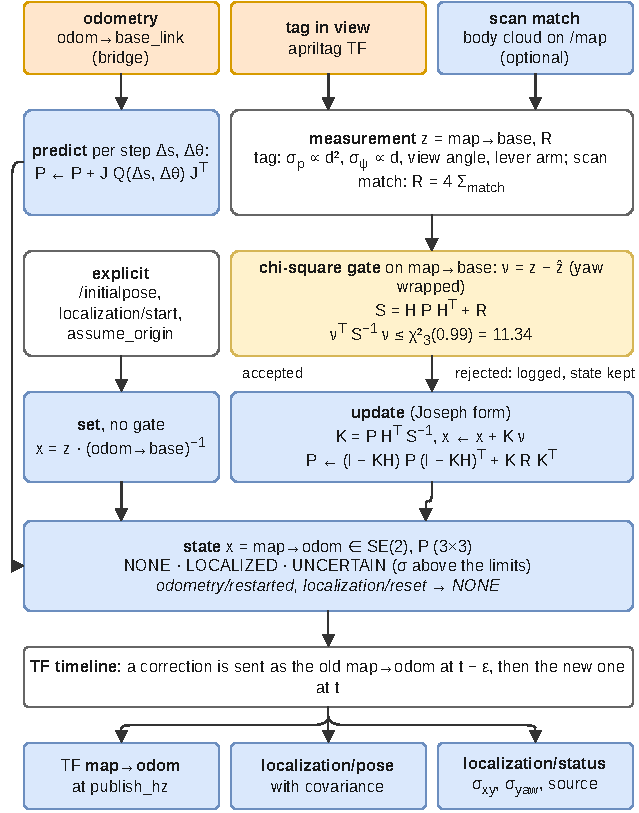
\includegraphics[width=0.62\textwidth]{localization_ekf}
  \caption{EKF over \frm{map}$\to$\frm{odom}: prediction from odometry motion, gated automatic
    corrections, explicit operator input and the TF timeline.}
  \label{fig:m-ekf}
\end{figure}

\subsection{Why}

In 0.1 one tag detection replaced \frm{map}$\to$\frm{odom} directly (finding L1). There was no
covariance, no fusion of detections and no correction between tags; detections were rejected
when the correction itself exceeded 0.5~m or 15° (review \#1), which rejected good fixes far
from the odometry origin and accepted small rotations that moved the robot metres. The errors
of a single detection propagate as
\begin{center}
\begin{tabular}{@{}llr@{}}
  \toprule
  Case & Parameters & Error \\
  \midrule
  PnP of a 16~cm tag, position $\approx d\,\delta$ & $d = 3$~m, $\delta = 3^\circ$ & 15.7~cm \\
  same & $d = 5$~m, $\delta = 2^\circ$ & 17.5~cm \\
  heading of \frm{map}$\to$\frm{odom}, $e_\perp \approx L\,\delta\psi$ & $L = 10$~m,
    $\delta\psi = 1^\circ$ & 17.5~cm \\
  same & $L = 30$~m, $\delta\psi = 1^\circ$ & 52.4~cm \\
  \bottomrule
\end{tabular}
\end{center}

\subsection{State and prediction}

The state is $\vect{x} = (x, y, \psi)$ of $\T{map}{odom}$ with a $3\times3$ covariance
$\mathbf{P}$. Given the odometry pose $\vect{o} = \T{odom}{base}$, the robot pose is
$h(\vect{x}) = \vect{x} \oplus \vect{o} = (x_b, y_b, \psi_b)$ and
\begin{equation}
  \mathbf{H} = \frac{\partial h}{\partial \vect{x}} =
  \begin{bmatrix} 1 & 0 & -(y_b - y) \\ 0 & 1 & x_b - x \\ 0 & 0 & 1 \end{bmatrix}.
\end{equation}
The third column is the lever arm: a rotation of \frm{map}$\to$\frm{odom} moves a robot far from
the \frm{odom} origin by a lot. Odometry motion is counted in steps (a robot standing still
never grows uncertain); for a step of distance $\Delta s$ and rotation $\Delta\theta$ the drift
of the robot pose
\begin{equation}
  \mathbf{Q} = \mathrm{diag}\big(\sigma_s^2\Delta s,\ \sigma_s^2\Delta s,\ \sigma_{\psi s}^2
  \Delta s + \sigma_{\psi\theta}^2 \Delta\theta\big)
\end{equation}
is mapped onto the state, $\mathbf{P} \leftarrow \mathbf{P} + \mathbf{H}^{-1}\mathbf{Q}
\mathbf{H}^{-\top}$. With $\sigma_s = 0.03$~m$/\sqrt{\mathrm{m}}$ the position uncertainty
grows to about 10~cm after 10~m.

\subsection{Update and gate}

A measurement $\vect{z}$ of \frm{map}$\to$\frm{base_link} with covariance $\mathbf{R}$, taken
while the odometry read $\vect{o}$, gives
\begin{equation}
  \vect{\nu} = \vect{z} - h(\vect{x})\ (\text{yaw wrapped}), \qquad
  \mathbf{S} = \mathbf{H}\mathbf{P}\mathbf{H}^\top + \mathbf{R}, \qquad
  d^2 = \vect{\nu}^\top\mathbf{S}^{-1}\vect{\nu}.
\end{equation}
Automatic sources pass only if $d^2 \le \chi^2_3(p)$ ($p$ = \param{estimator.gate_confidence},
0.99: 11.34)~\cite{barshalom2001estimation}. The gate opens as the uncertainty grows after a
long drive and is tight after a correction. An accepted measurement updates
\begin{equation}
  \mathbf{K} = \mathbf{P}\mathbf{H}^\top\mathbf{S}^{-1}, \quad
  \vect{x} \leftarrow \vect{x} + \mathbf{K}\vect{\nu}, \quad
  \mathbf{P} \leftarrow (\mathbf{I} - \mathbf{K}\mathbf{H})\mathbf{P}(\mathbf{I} -
  \mathbf{K}\mathbf{H})^\top + \mathbf{K}\mathbf{R}\mathbf{K}^\top
\end{equation}
(Joseph form, symmetric by construction), followed by a floor on the robot pose covariance
(\param{estimator.min_sigma_xy}, \param{estimator.min_sigma_yaw_deg}) against overconfidence. The reported sigmas are
those of the robot pose, $\mathbf{H}\mathbf{P}\mathbf{H}^\top$: $\sigma_{xy}$ is the square
root of the largest eigenvalue of its position block.

\textbf{States.} \code{NONE} before the first fix (sigmas infinite), \code{LOCALIZED},
\code{UNCERTAIN} when $\sigma_{xy}$ exceeds \param{estimator.max_sigma_xy} or $\sigma_\psi$
exceeds \param{estimator.max_sigma_yaw_deg}.

\subsection{Sources}

\begin{description}
  \item[Tag.] A detection $\T{cam}{tag}$ of a tag with known $\T{map}{tag}$ gives
    \begin{equation}
      \T{map}{base} = \T{map}{tag}\,\big(\T{base}{cam}\,\T{cam}{tag}\big)^{-1},
    \end{equation}
    computed in SE(3) because the optical frame (z forward, x right, y down) is never planar,
    then flattened to $(x, y, \psi)$. Detections farther than \param{tag.max_distance_m} or
    seen more obliquely than \param{tag.max_view_angle_deg} are ignored. The noise grows with
    distance $d$ (at least 0.3~m) and view angle $\alpha$:
    $\sigma_p = \sigma_{p,1}\,d^2/\cos\alpha$, $\sigma_\psi = \sigma_{\psi,1}\,d/\cos\alpha$.
    A heading error rotates the robot about the tag: with $\vect{v}$ the vector from the robot
    to the tag and $\vect{l} = (v_y, -v_x)$,
    \begin{equation}
      \mathbf{R} = \begin{bmatrix} \sigma_p^2\mathbf{I} + \sigma_\psi^2\vect{l}\vect{l}^\top &
      \sigma_\psi^2\vect{l} \\ \sigma_\psi^2\vect{l}^\top & \sigma_\psi^2 \end{bmatrix}.
    \end{equation}
    Far tags therefore count little, and a test with the real optical rotation
    $(-\pi/2, 0, -\pi/2)$ and non-zero yaws checks the geometry (review \#15).
  \item[Pose estimate.] \topic{/initialpose} (RViz 2D Pose Estimate). RViz sends a fixed UI
    covariance whatever the operator meant, so the operator is trusted (5~cm, 2°); a tighter
    covariance from another client (a simulator) is used as given. Applied without gate.
  \item[Scan match] (optional, \param{scan_match.enabled}). The registered body cloud is put
    into the level \frm{odom} with its full 3D pose, a height band above the floor is kept, the
    points are expressed in the planar base frame and matched against \topic{/map} with the
    correlative matcher of \pkg{dharma_utils}~\cite{olson2009csm} (coarse to fine on a
    likelihood field); the covariance of the score surface, scaled by 4, is $\mathbf{R}$.
  \item[Explicit.] \topic{localization/start} (localize from a tag in view),
    \topic{localization/assume_origin} (\frm{map}$\to$\frm{odom} = identity, for a new map) and
    a pose estimate set the state without gate, so a far but consistent tag that the gate
    rejects (after a kidnapping or a wrong pose estimate) still relocalizes on request.
\end{description}

\subsection{Publication without interpolation ramps}

tf2 interpolates between the two samples around a lookup time. If \frm{map}$\to$\frm{odom}
changed between two periodic samples, lookups in that interval would see a blend of the old and
the new value, mapping scans to poses that never existed (findings T1/T3, review \#14). A
correction is therefore published as the previous value at $t - \epsilon$ followed by the new
value at $t$ ($\epsilon = 1$~ms), and periodic samples are strictly increasing in time.

\section{Fiducial tags}

\code{record_tags} averages the map pose of the visible \param{tag.frames} over
\param{tag.record_duration_sec} and merges them into the tags file. It writes the anchors of a
site, so it refuses unless the state is \code{LOCALIZED} and never records the tag the current
\frm{map}$\to$\frm{odom} was derived from (circular, review \#2). Recordings with fewer than
\param{tag.record_min_samples} samples or a larger spread than the limits are refused. It runs
as a session over the node's timers in its own callback group (no sleep in a callback, finding
L2), so \frm{map}$\to$\frm{odom} keeps flowing at \param{publish_hz} while it records. Reads are
tolerant: a corrupt tags file is reported (\texttt{success: false}) and left untouched (review
\#3); every write keeps a \code{.bak}. \code{load_tags} accepts only paths that resolve inside
\param{sites_dir} (review \#12); \code{~} is expanded (review \#11).

\section{Interfaces}

\begin{center}
\begin{tabularx}{\textwidth}{@{}p{0.31\textwidth}p{0.27\textwidth}X@{}}
  \toprule
  Interface & Type & \\
  \midrule
  \topic{localization/start} & Trigger & localize from a tag in view, explicitly \\
  \topic{localization/reset} & Trigger & forget \frm{map}$\to$\frm{odom} \\
  \topic{localization/assume_origin} & Trigger & \frm{map}$\to$\frm{odom} = identity \\
  \topic{localization/record_tags} & Trigger & record the visible tags \\
  \topic{localization/load_tags} & LoadFile & switch the tags file (inside \param{sites_dir}) \\
  \topic{localization/status} & LocalizationStatus & latched: state, source, sigmas, time
    since the last correction \\
  \topic{localization/pose} & PoseWithCovariance\-Stamped & robot pose with covariance \\
  \topic{localization/tag_markers} & MarkerArray & known tags \\
  in: \topic{odometry/restarted}, \topic{/initialpose}, IMU, \topic{/map},
    \topic{/cloud_registered_body} & & \\
  \bottomrule
\end{tabularx}
\end{center}

\section{Parameters}

\readonlynote

% Generated by docs/manual/tools/reference.py; do not edit.
\begin{small}
\begin{longtable}{@{}p{0.28\textwidth}p{0.12\textwidth}p{0.08\textwidth}p{0.11\textwidth}p{0.29\textwidth}@{}}
\toprule
Parameter & Default & Unit & Range & Description \\
\midrule
\endhead
\bottomrule
\endfoot
\multicolumn{5}{@{}l}{\textbf{localization\_node}} \\
\code{sites_dir}$^\dagger$ & \code{~/dharma/map} &  &  & load\_tags paths must be inside \\
\code{tags_file}$^\dagger$ & \code{""} &  &  & tags file at start (empty: none until load\_tags) \\
\code{lio_odom_frame}$^\dagger$ & \code{camera_init} &  &  & LIO world frame \\
\code{lio_body_frame}$^\dagger$ & \code{body} &  &  & LIO body frame (the IMU) \\
\code{imu_frame}$^\dagger$ & \code{livox_imu_frame} &  &  & URDF frame of the LIO body \\
\code{publish_hz}$^\dagger$ & 20 & Hz & 1\,..\,200 & map->odom on /tf \\
\code{pose_hz}$^\dagger$ & 10 & Hz & 0\,..\,100 & localization/pose; 0: off \\
\code{assume_start_origin}$^\dagger$ & false &  &  & the odom origin is the map origin at start (no tag needed) \\
\code{estimator.sigma_xy_per_sqrt_m} & 0.03 & m/sqrt(m) & 0\,..\,1 & position drift: 1-sigma after 1 m of travel \\
\code{estimator.sigma_yaw_deg_per_sqrt_m} & 0.1 & deg/sqrt(m) & 0\,..\,10 & heading drift per metre of travel \\
\code{estimator.sigma_yaw_deg_per_sqrt_rad} & 0.5 & deg/sqrt(rad) & 0\,..\,10 & heading drift per radian turned \\
\code{estimator.gate_confidence} & 0.99 &  & 0.95, 0.99, 0.999 & chi-square gate (3 dof) of automatic corrections \\
\code{estimator.max_sigma_xy} & 0.5 & m & 0.01\,..\,100 & above: state UNCERTAIN (position) \\
\code{estimator.max_sigma_yaw_deg} & 10 & deg & 0.1\,..\,180 & above: state UNCERTAIN (heading) \\
\code{estimator.min_sigma_xy} & 0.01 & m & 0\,..\,1 & floor after a correction (no overconfidence) \\
\code{estimator.min_sigma_yaw_deg} & 0.25 & deg & 0\,..\,10 & heading floor after a correction \\
\code{estimator.motion_step_m} & 0.05 & m & 0.001\,..\,1 & odometry motion counted in steps (jitter-free) \\
\code{estimator.motion_step_deg} & 2 & deg & 0.01\,..\,45 & odometry rotation counted in steps \\
\code{tag.camera_frame}$^\dagger$ & \code{camera_color_optical_frame} &  &  & frame the detector puts the tags under \\
\code{tag.frames} & [\code{base_map}, \code{charging_dock}] &  &  & tag TF frames to record (the detector tag frames) \\
\code{tag.max_age_sec} & 0.5 & s & 0.01\,..\,10 & older detections ignored \\
\code{tag.max_distance_m} & 4 & m & 0.1\,..\,50 & farther tags ignored \\
\code{tag.max_view_angle_deg} & 60 & deg & 1\,..\,89 & tags seen more obliquely are ignored \\
\code{tag.sigma_xy_at_1m} & 0.02 & m & 0.001\,..\,1 & position sigma at 1 m, grows with distance\textasciicircum{}2 \\
\code{tag.sigma_yaw_deg_at_1m} & 1 & deg & 0.01\,..\,30 & heading sigma at 1 m, grows with distance \\
\code{tag.update_hz}$^\dagger$ & 10 & Hz & 0.5\,..\,50 & tag checks \\
\code{tag.min_interval_sec} & 0.5 & s & 0\,..\,60 & per tag, between two fused detections \\
\code{tag.auto_localize} & true &  &  & while not localized: localize from any visible tag \\
\code{tag.auto_correct} & true &  &  & while localized: fuse visible tags through the gate \\
\code{tag.record_duration_sec} & 2 & s & 0.2\,..\,60 & record\_tags \\
\code{tag.record_min_samples} & 5 &  & 1\,..\,1000 & detections needed per tag \\
\code{tag.record_max_std_m} & 0.05 & m & 0.001\,..\,1 & noisier recordings are refused \\
\code{tag.record_max_std_deg} & 3 & deg & 0.01\,..\,45 & noisier recordings are refused (heading) \\
\code{tag.marker_size} & 0.15 & m & 0.01\,..\,2 & tag plate in RViz \\
\code{scan_match.enabled}$^\dagger$ & false &  &  & match the registered cloud against /map \\
\code{scan_match.cloud_topic}$^\dagger$ & \code{/cloud_registered_body} &  &  & deskewed cloud in the LIO body frame \\
\code{scan_match.rate_hz} & 1 & Hz & 0.05\,..\,10 & matches per second, at most \\
\code{scan_match.min_height_m} & 0.1 & m & -1\,..\,5 & band above the floor \\
\code{scan_match.max_height_m} & 1.5 & m & 0\,..\,10 & band above the floor \\
\code{scan_match.max_range_m} & 15 & m & 0.5\,..\,200 & farther points ignored \\
\code{scan_match.xy_window_m} & 0.3 & m & 0.05\,..\,5 & search window \\
\code{scan_match.yaw_window_deg} & 6 & deg & 0.5\,..\,45 & search window \\
\code{scan_match.min_score} & 0.5 &  & 0\,..\,1 & mean likelihood needed \\
\code{scan_match.covariance_scale} & 4 &  & 1\,..\,1000 & inflates the match covariance (correlated points) \\
\code{scan_match.occupied_threshold} & 65 &  & 1\,..\,100 & occupancy value of an obstacle \\
\code{leveling.enabled}$^\dagger$ & true &  &  & level odom with the IMU (off: odom = base) \\
\code{leveling.imu_topic}$^\dagger$ & \code{/livox/imu} &  &  & IMU in the LIO body frame axes \\
\code{leveling.window_sec} & 1 & s & 0.1\,..\,10 & still window \\
\code{leveling.max_rate_deg_s} & 3 & deg/s & 0.1\,..\,90 & still: gyro rate below this \\
\code{leveling.max_accel_spread} & 0.03 &  & 0.001\,..\,0.5 & still: accelerometer std / mean norm below this \\
\code{leveling.max_tilt_deg} & 20 & deg & 1\,..\,60 & larger start tilts are refused (wrong frame?) \\
\code{leveling.timeout_sec} & 15 & s & 0\,..\,600 & then the bridge goes up unleveled; 0: wait \\
\end{longtable}
\end{small}


\chapter{Perception}
\label{ch:perception}

\pkg{dharma_perception} turns the LiDAR into two sector scans in \param{robot.frames.base}: a
front scan for reactive avoidance (\topic{perception/sector_scan}) and a fail-safe 360° scan for
the protective field and the follower's motion guard (\topic{perception/safety_scan}). It also
throttles the camera for the fiducial detector.

\section{Sector scan semantics}

A \code{SectorScan} holds the nearest obstacle per angular sector; sector $i$ is centred at
\code{angle_min} $+ (i + \tfrac12)$ \code{angle_increment}. \texttt{ranges[i] >= range\_max} means
nothing within range; \texttt{ranges[i] <= BLOCKED} (0) or NaN means blocked or unknown, and
\emph{every consumer treats it as an obstacle at the robot}. Every sector is \code{BLOCKED}
when:
\begin{itemize}
  \item the LiDAR is blind: fewer than \param{blind.min_points} points off the robot body, or
    (with \param{blind.min_region_points}) one of \param{blind.regions} azimuth regions empty;
  \item the sensor mount transform or, with \param{filter.level_source} \code{tf}, the roll and
    pitch of the base (\frm{odom}$\to$\frm{base_link}) is missing;
  \item processing raised an exception, or no usable cloud arrived for
    \param{input.timeout_sec} (driver down, only malformed messages).
\end{itemize}
In 0.1 an all-zero scan was read as free by the protective field (review B1) and NaN sectors as
free by the follower (F1); this convention removes both.

\section{Pipeline}

\begin{enumerate}
  \item \textbf{Parse.} The serialized Livox \code{CustomMsg} is read with numpy (no per-point
    Python objects; every length validated, both endiannesses). PointCloud2 goes through
    \code{dharma_utils.ros.pointcloud.read_xyz}. A malformed message is dropped with a
    throttled error (review \#4).
  \item \textbf{Livox noise.} The tag byte marks each point per field (bits 0--1 adhesion
    between objects, 2--3 rain, fog or dust, 4--5 other; 0 high, 1 medium, 2 low confidence).
    Points at \param{filter.noise_level} in the enabled fields are dropped (review \#12).
  \item \textbf{Self filter.} Points inside \param{robot.footprint} grown by
    \param{filter.self_margin}.
  \item \textbf{Level.} Points in \frm{base_link} are rotated by the roll and pitch of the base
    in \frm{odom} at the cloud stamp, so the band is relative to the floor while the gait pitches
    the body (finding P1).
  \item \textbf{Height band.} \param{filter.height_min} to \param{filter.height_max} above the
    floor, the floor being \param{robot.base_height} below \frm{base_link}. Optional
    \param{filter.ground_segmentation} estimates the floor per cell (lowest point within a
    maximum step) for ramps and thresholds.
  \item \textbf{Sectors.} Each range is the $k$-th nearest point of the sector (\param{front.k},
    \param{safety.k}, default 2): a single dust return does not stop the robot; a sector with
    fewer than $k$ points is free.
  \item \textbf{Obstacle memory.} Confirmed safety points are kept in \frm{odom} for
    \param{memory.memory_sec} and merged into the safety scan while they are hidden below the
    lowest beam; an odometry jump clears the memory (review B4).
\end{enumerate}

\textbf{Why levelling matters.} For a flat floor and \frm{base_link} at height $h$ pitched by
$\vartheta$, a floor point at horizontal range $r$ appears at $z \approx -h + r\sin\vartheta$ and
enters the band at
\begin{equation}
  r > r_{\mathrm{false}} = \frac{h + z_{\min}}{\sin\vartheta}.
\end{equation}
\begin{center}
\begin{tabular}{@{}lrrrr@{}}
  \toprule
  Band margin $h + z_{\min}$ & $\vartheta = 1^\circ$ & $2^\circ$ & $3^\circ$ & $5^\circ$ \\
  \midrule
  10~cm & 5.7~m & 2.9~m & 1.9~m & 1.15~m \\
  5~cm & 2.9~m & 1.4~m & 0.96~m & 0.57~m \\
  \bottomrule
\end{tabular}
\end{center}
A trotting legged robot pitches by a few degrees, so in \frm{base_link} the floor became an
obstacle within the 4~m safety range (false stops), and pitching up hid low obstacles (missed
detections). The 0.1 configuration also assumed $h = 0.35$~m in one file and 0.30~m in another;
both now come from the profile.

\section{Limits}
\label{sec:perception-limits}

\begin{itemize}
  \item \textbf{Near-field blind zone.} A Mid-360 sees down to $-7^\circ$: mounted 0.53~m above
    the floor it sees a 10~cm object only beyond about 3.5~m. The memory keeps objects seen
    earlier, but an object that appears inside the zone (placed there, or the robot switched on
    next to it) is not seen. Use a pitched mount or a near-field sensor (bumper, ToF, 2D
    scanner) where this matters.
  \item \textbf{Negative obstacles} (stairs down, holes, platform edges) are not detected:
    missing floor is not an obstacle.
  \item \textbf{Motion distortion.} The scan is not deskewed: a Mid-360 frame spans 100~ms, so
    a point is up to $v \cdot 0.1$~m off (8~cm at 0.8~m/s) and turning at $\omega$ moves a point
    at range $r$ by up to $0.1\,\omega r$. The latency from the first point to the published scan
    is the frame (100~ms), driver and transport (about 5--10~ms) and processing (about
    10--15~ms for 20k points on one desktop core); \param{robot.limits.reaction_time} must stay
    above it and the field margins above the distortion.
  \item \textbf{Quantization.} The nearest point of a sector stands for the whole sector: 72
    safety sectors are 5° wide (lateral error up to $r\Delta\theta/2$: 8.7~cm at 2~m, 17.5~cm at
    4~m). Raise \param{safety.num_sectors} for a finer field.
  \item This is a software channel; it does not replace a safety-rated scanner
    (Section~\ref{sec:two-channel}).
\end{itemize}

\section{Nodes and parameters}

\begin{center}
\begin{tabularx}{\textwidth}{@{}p{0.30\textwidth}X@{}}
  \toprule
  Node & Role \\
  \midrule
  \code{lidar_sector_node} & Livox \code{CustomMsg} (raw bytes, default) or PointCloud2 in;
    \topic{perception/sector_scan}, \topic{perception/safety_scan}, \topic{perception/obstacles}
    out \\
  \code{apriltag_throttle} & camera image and info in, image at \code{rate_hz} out \\
  \code{apriltag} (\code{apriltag_ros}) & tag frames on TF for localization \\
  \bottomrule
\end{tabularx}
\end{center}

\readonlynote

% Generated by docs/manual/tools/reference.py; do not edit.
\begin{small}
\begin{longtable}{@{}p{0.28\textwidth}p{0.12\textwidth}p{0.08\textwidth}p{0.11\textwidth}p{0.29\textwidth}@{}}
\toprule
Parameter & Default & Unit & Range & Description \\
\midrule
\endhead
\bottomrule
\endfoot
\multicolumn{5}{@{}l}{\textbf{lidar\_sector\_node}} \\
\code{input.type}$^\dagger$ & \code{livox} &  & livox, pointcloud2 & livox: raw Livox CustomMsg bytes; pointcloud2: any PointCloud2 \\
\code{input.livox_topic}$^\dagger$ & \code{livox/lidar} &  &  & Livox CustomMsg topic \\
\code{input.pointcloud_topic}$^\dagger$ & \code{/cloud_registered_body} &  &  & PointCloud2 topic (frame fixed to the robot) \\
\code{input.frame}$^\dagger$ & \code{livox_frame} &  &  & sensor frame when the header has none \\
\code{input.timeout_sec}$^\dagger$ & 0.5 & s & 0.05\,..\,10 & no usable cloud for this long: every sector is published BLOCKED \\
\code{front.num_sectors}$^\dagger$ & 32 &  & 1\,..\,1440 & sectors over the fov \\
\code{front.fov_deg}$^\dagger$ & 180 & deg & 1\,..\,360 & centred ahead \\
\code{front.range_min}$^\dagger$ & 0.1 & m & 0\,..\,10 & closer: ignored \\
\code{front.range_max}$^\dagger$ & 8 & m & 0.1\,..\,100 & free beyond \\
\code{front.k}$^\dagger$ & 2 &  & 1\,..\,100 & a sector needs k points; its range is the k-th nearest \\
\code{safety.enabled}$^\dagger$ & true &  &  & publish perception/safety\_scan \\
\code{safety.num_sectors}$^\dagger$ & 72 &  & 4\,..\,1440 & sectors over 360 deg \\
\code{safety.range_min}$^\dagger$ & 0.1 & m & 0\,..\,10 & closer: ignored \\
\code{safety.range_max}$^\dagger$ & 4 & m & 0.1\,..\,100 & free beyond \\
\code{safety.k}$^\dagger$ & 2 &  & 1\,..\,100 & a sector needs k points; its range is the k-th nearest \\
\code{filter.self_margin}$^\dagger$ & 0.05 & m & 0\,..\,1 & footprint grown by this is the robot \\
\code{filter.level_source}$^\dagger$ & \code{tf} &  & tf, none & tf: roll/pitch of base in odom (unknown -> BLOCKED); none: base assumed level \\
\code{filter.tilt_max_age}$^\dagger$ & 0.2 & s & 0.01\,..\,5 & oldest odom->base usable for leveling \\
\code{filter.height_min}$^\dagger$ & 0.1 & m & -1\,..\,3 & band bottom above the floor \\
\code{filter.height_max}$^\dagger$ & 1.6 & m & 0\,..\,5 & band top above the floor \\
\code{filter.ground_segmentation}$^\dagger$ & false &  &  & estimate the floor height per cell (ramps, uneven floors) \\
\code{filter.ground_cell}$^\dagger$ & 0.3 & m & 0.05\,..\,5 & ground segmentation cell size \\
\code{filter.ground_max_step}$^\dagger$ & 0.05 & m & 0\,..\,0.5 & largest local floor offset accepted \\
\code{filter.drop_adhesion_noise}$^\dagger$ & true &  &  & Livox tag bits 0-1 (glue points) \\
\code{filter.drop_particle_noise}$^\dagger$ & true &  &  & Livox tag bits 2-3 (rain, dust) \\
\code{filter.drop_other_noise}$^\dagger$ & false &  &  & Livox tag bits 4-5 (other) \\
\code{filter.noise_level}$^\dagger$ & 2 &  & 1\,..\,2 & drop at this tag confidence: 1 medium, 2 low \\
\code{memory.enabled}$^\dagger$ & true &  &  & remember obstacles that left the view \\
\code{memory.memory_sec}$^\dagger$ & 10 & s & 0\,..\,60 & remembered points decay after this \\
\code{memory.radius}$^\dagger$ & 5 & m & 0.1\,..\,20 & points this close are remembered (merged only while below the lowest beam) \\
\code{memory.resolution}$^\dagger$ & 0.05 & m & 0.01\,..\,1 & memory cell size \\
\code{memory.max_cells}$^\dagger$ & 20000 &  & 100\,..\,1e+06 & memory size bound \\
\code{memory.lower_fov_deg}$^\dagger$ & -7 & deg & -90\,..\,0 & lowest beam elevation of the sensor (Mid-360: -7), for the near-field blind zone \\
\code{memory.max_jump}$^\dagger$ & 0.3 & m & 0\,..\,10 & odom jump beyond the motion: forget \\
\code{blind.min_points}$^\dagger$ & 100 &  & 0\,..\,1e+06 & fewer valid points in a cloud: blind \\
\code{blind.regions}$^\dagger$ & 4 &  & 1\,..\,36 & azimuth regions around the sensor z axis \\
\code{blind.min_region_points}$^\dagger$ & 0 &  & 0\,..\,100000 & fewer points in any region: blind (0: off) \\
\code{publish_markers}$^\dagger$ & true &  &  & perception/obstacles for RViz \\
\end{longtable}
\end{small}


\chapter{Mapping and sites}
\label{ch:mapping}

\pkg{dharma_mapping} records occupancy maps from the LiDAR-inertial odometry, manages sites
(one directory per mapped place with its map, the fiducials that anchor it and its routes) and
teaches routes.

\section{Sites}

\begin{lstlisting}
<sites_dir>/<site>/
  map.yaml, map.pgm            occupancy map (map_server format)
  map.yaml.bak, map.pgm.bak    the previous map (a loadable pair)
  tags.json                    fiducial poses in the map frame (localization/record_tags)
  routes/<date>_<time>.csv     taught routes (x, y, yaw_deg, dwell_sec > 0: stop point)
  backup-<time>[-n]/           what a mapping reset archived
\end{lstlisting}

A site's map frame is the frame its fiducials were recorded in. Site names match
\code{^[a-z0-9][a-z0-9_-]{0,47}$}; every path is derived from \param{sites_dir} and a site name,
never taken from a request (review \#12). The map pair is written crash safe: a temporary
directory, fsync, rename; the YAML records the image size and a CRC, so a torn pair is refused
on load and the \code{.bak} pair is used (review \#5). A reset archives the old site into a
unique \code{backup-<time>[-n]} directory, after all preconditions were checked (review \#13).
Broken site files are notes in \topic{site/status}, never a crash (review \#7).

\section{Occupancy grid}

\subsection{Log-odds model}

For a cell with occupancy probability $p$ the grid stores $l = \log\frac{p}{1-p}$:
\begin{equation}
  l_t = \mathrm{clip}\Big(l_{t-1} + \begin{cases} l_{\mathrm{hit}} = 0.85 & \text{cell hit}\\
  l_{\mathrm{miss}} = -0.4 & \text{cell crossed by a ray} \end{cases},\ [-2.0,\ 3.5]\Big).
\end{equation}
A cell is occupied above $\mathrm{logit}(0.65) = 0.619$ (a single hit suffices) and free below
$\mathrm{logit}(0.35) = -0.619$ (two rays). A saturated cell becomes free only after
$\lceil (3.5 + 0.619)/0.4 \rceil = 11$ crossing rays, about 5.5~s of observation at 2~Hz, so a
person standing still for long while mapping stays in the map. Free space is carved only up to
the nearest hit per angular bin (\param{scan.angular_bins}, 720): glass and open doors are not
cleared. This is conservative by design.

\subsection{Which scans and points are integrated}

\begin{itemize}
  \item \textbf{Height band.} Points between \param{scan.height_min} and \param{scan.height_max}
    above the floor, measured in the map frame (floor = \frm{base_link} height in the map minus
    \param{robot.base_height}). This needs a level map frame: localization levels \frm{odom}
    with the IMU, so map and \frm{odom} are gravity-aligned and a pitching body never turns the
    floor into walls (finding O1).
  \item \textbf{Self filter.} Points inside the footprint grown by \param{scan.self_margin}.
  \item \textbf{Correction gate.} A scan is skipped when \frm{map}$\to$\frm{odom} changes within
    \param{gate.correction_window_sec} around it by more than \param{gate.correction_tol_m} or
    \param{gate.correction_tol_deg}: its TF pose may be the old, the new or a blend of both
    (review \#14).
  \item \textbf{Jump gate.} A sensor that moved more than $d_{\max} + v_{\max}\Delta t$ (or turned
    more than $\psi_{\max} + \omega_{\max}\Delta t$) since the previous scan jumped (odometry
    reset, bad correction). Integration then holds until a scan agrees with the map at its pose
    again (score above \param{gate.resume_score}), so a jump never smears the map or grows the
    grid (finding M1, review \#8).
  \item \textbf{Growth cap.} The grid grows in steps of \param{grid.grow_m} and never beyond
    \param{grid.max_size_m} per side; hits beyond are dropped. In 0.1 a 300~m odometry jump grew
    the grid to 109~MB.
  \item \textbf{Optional refinement} (\param{refine.enabled}, off by default). The TF pose is
    matched on the current grid before integrating, gated on score and ambiguity. It sharpens
    walls under small pose errors, but its ambiguity gate separates a corridor from a room only
    by a factor of two, so it stays off until a test shows it helps.
\end{itemize}

There is no loop closure: map quality equals odometry plus localization quality. A pose graph
over scan matches, with tags as landmarks, is future work.

\subsection{Mapping sessions}

\code{mapping/start} on a new site (or with \code{reset}) maps in the current map frame, or
takes the current pose as origin when not localized. Continuing a site that already has a map
or tags needs the robot localized in \emph{its} frame: on one of its tags or by a pose estimate
on its map; an \code{origin} localization at boot does not count (review \#9). The session
remembers its site and refuses a save into another one; a stop that the mapper does not confirm
is a failure (review \#4).

\section{Route teaching}

\code{route_recorder_node} (moved here from \pkg{dharma_odometry}: routes are site data) samples
\frm{map}$\to$\frm{base_link} while \code{route/start} is active and writes
\code{<site>/routes/<date>_<time>.csv} incrementally and atomically
(\code{dharma_utils.io.write_route}). It records only while \topic{localization/status} is
\code{LOCALIZED} (a TF that exists is not a localization); \code{route/mark_stop_point} makes the
current pose a stop point with \code{dwell_sec}; file errors make the service fail instead of
killing the node.

\section{Interfaces}

\begin{center}
\begin{tabularx}{\textwidth}{@{}p{0.30\textwidth}p{0.24\textwidth}X@{}}
  \toprule
  Interface & Type & \\
  \midrule
  \topic{/map} & OccupancyGrid, latched & the site map, or the live grid while mapping (only
    publisher: site manager) \\
  \topic{mapping/grid} & OccupancyGrid, latched & the live grid \\
  \topic{mapping/status} & MappingStatus, latched & scans, rejected, size, known area \\
  \topic{site/status} & SiteStatus, latched & site, sites, map, mapping, tags, routes, notes \\
  \topic{route/saved} & String & path of a saved route \\
  \topic{site/list}, \topic{site/load} & ListSites, LoadSite & another site resets localization \\
  \topic{mapping/start} & StartMapping & \code{reset} archives the old site \\
  \topic{mapping/stop}, \topic{mapping/save} & Trigger & \\
  \topic{route/start}, \topic{route/stop} & Trigger & refused unless \code{LOCALIZED} \\
  \topic{route/mark_stop_point} & MarkStopPoint & \\
  \bottomrule
\end{tabularx}
\end{center}

Used: \topic{localization/status}, \topic{localization/load_tags} (a path inside
\param{sites_dir}), \topic{localization/start}, \topic{reset}, \topic{assume_origin}. Internal:
\topic{grid_mapper/start|stop|save|load} (site names only).

\section{Parameters}

\readonlynote

% Generated by docs/manual/tools/reference.py; do not edit.
\begin{small}
\begin{longtable}{@{}p{0.28\textwidth}p{0.12\textwidth}p{0.08\textwidth}p{0.11\textwidth}p{0.29\textwidth}@{}}
\toprule
Parameter & Default & Unit & Range & Description \\
\midrule
\endhead
\bottomrule
\endfoot
\multicolumn{5}{@{}l}{\textbf{grid\_mapper\_node}} \\
\code{sites_dir}$^\dagger$ & \code{~/dharma/map} &  &  & one directory per site \\
\code{cloud_topic}$^\dagger$ & \code{/cloud_registered_body} &  &  & deskewed scan in a frame fixed to the robot \\
\code{rate_hz}$^\dagger$ & 2 & Hz & 0.1\,..\,50 & scans integrated \\
\code{publish_hz}$^\dagger$ & 1 & Hz & 0.1\,..\,10 & mapping/grid while mapping \\
\code{max_cloud_age_sec}$^\dagger$ & 1 & s & 0.1\,..\,30 & scans without TF this long: dropped \\
\code{save_margin_m}$^\dagger$ & 1 & m & 0\,..\,20 & unknown border kept when saving \\
\code{grid.resolution}$^\dagger$ & 0.05 & m & 0.01\,..\,1 & cell size \\
\code{grid.initial_size_m}$^\dagger$ & 20 & m & 1\,..\,1000 & side of the first grid \\
\code{grid.grow_m}$^\dagger$ & 5 & m & 0.1\,..\,100 & extra border added when it grows \\
\code{grid.max_size_m}$^\dagger$ & 150 & m & 1\,..\,2000 & largest side; hits beyond are dropped (memory: (size / resolution)\textasciicircum{}2 * 4 bytes) \\
\code{grid.log_odds_hit}$^\dagger$ & 0.85 &  & 0\,..\,10 & added per hit \\
\code{grid.log_odds_miss}$^\dagger$ & -0.4 &  & -10\,..\,0 & added per crossing \\
\code{grid.log_odds_min}$^\dagger$ & -2 &  & -50\,..\,0 & clamp, free side \\
\code{grid.log_odds_max}$^\dagger$ & 3.5 &  & 0\,..\,50 & clamp, occupied side \\
\code{grid.occupied_threshold}$^\dagger$ & 0.65 &  & 0.5\,..\,1 & probability above which a cell is occupied \\
\code{grid.free_threshold}$^\dagger$ & 0.35 &  & 0\,..\,0.5 & probability below which a cell is free \\
\code{scan.voxel}$^\dagger$ & 0.05 & m & 0\,..\,1 & downsampling, 0: off \\
\code{scan.min_range}$^\dagger$ & 0.3 & m & 0\,..\,10 & from the sensor \\
\code{scan.max_range}$^\dagger$ & 15 & m & 0.5\,..\,200 & hits and free space beyond: ignored \\
\code{scan.angular_bins}$^\dagger$ & 720 &  & 8\,..\,7200 & free space is carved to the nearest hit per bin \\
\code{scan.height_min}$^\dagger$ & 0.05 & m & -1\,..\,3 & band bottom above the floor \\
\code{scan.height_max}$^\dagger$ & 1.5 & m & 0\,..\,10 & band top above the floor \\
\code{scan.self_margin}$^\dagger$ & 0.05 & m & 0\,..\,1 & footprint grown by this is the robot \\
\code{gate.max_jump_m}$^\dagger$ & 0.5 & m & 0.01\,..\,100 & sensor motion between scans beyond this plus max speed * dt: a jump \\
\code{gate.max_jump_deg}$^\dagger$ & 30 & deg & 1\,..\,180 & yaw beyond this plus max\_wz * dt \\
\code{gate.correction_window_sec}$^\dagger$ & 0.5 & s & 0\,..\,10 & map->odom compared this long before the scan and at the newest time \\
\code{gate.correction_tol_m}$^\dagger$ & 0.02 & m & 0\,..\,1 & map->odom change counted as correction \\
\code{gate.correction_tol_deg}$^\dagger$ & 0.5 & deg & 0\,..\,10 & map->odom yaw change, same \\
\code{gate.resume_score}$^\dagger$ & 0.6 &  & 0\,..\,1 & after a jump, a scan agreeing this well with the map resumes integration \\
\code{refine.enabled}$^\dagger$ & false &  &  & match each scan on the current grid \\
\code{refine.xy_window}$^\dagger$ & 0.2 & m & 0.01\,..\,2 & search window around the TF pose \\
\code{refine.yaw_window_deg}$^\dagger$ & 3 & deg & 0.1\,..\,30 & yaw search window \\
\code{refine.min_score}$^\dagger$ & 0.5 &  & 0\,..\,1 & mean likelihood needed to accept a match \\
\code{refine.max_sigma_m}$^\dagger$ & 0.045 & m & 0.001\,..\,1 & largest accepted position sigma \\
\code{refine.min_occupied}$^\dagger$ & 200 &  & 10\,..\,1e+06 & occupied cells near the robot needed to match \\
\multicolumn{5}{@{}l}{\textbf{site\_manager\_node}} \\
\code{sites_dir}$^\dagger$ & \code{~/dharma/map} &  &  & one directory per site \\
\code{site}$^\dagger$ & \code{""} &  &  & site loaded at start; empty: the one of the last run \\
\code{state_file}$^\dagger$ & \code{~/.dharma/site} &  &  & remembers the active site \\
\code{start_mapping}$^\dagger$ & false &  &  & map `site` at start when it is a new site (mapping mode) \\
\code{service_timeout_sec}$^\dagger$ & 5 & s & 0.5\,..\,60 & waiting for localization and mapper \\
\code{refresh_sec}$^\dagger$ & 2 & s & 0.5\,..\,60 & site/status refresh (tags, routes) \\
\multicolumn{5}{@{}l}{\textbf{route\_recorder\_node}} \\
\code{sites_dir}$^\dagger$ & \code{~/dharma/map} &  &  & routes go to <sites\_dir>/<site>/routes \\
\code{output_path}$^\dagger$ & \code{""} &  &  & directory for routes while no site is active; empty: refuse \\
\code{min_spacing_m} & 0.2 & m & 0.01\,..\,10 & a new waypoint after this much motion \\
\code{record_rate_hz}$^\dagger$ & 10 & Hz & 0.5\,..\,100 & pose sampling while recording \\
\code{flush_sec} & 2 & s & 0.1\,..\,60 & the route file is rewritten at most this often \\
\code{max_tf_age_sec} & 0.5 & s & 0.01\,..\,10 & older map->base: no sample \\
\end{longtable}
\end{small}


\chapter{Navigation}
\label{ch:navigation}

\pkg{dharma_navigation} plans paths on the site map, loads taught routes, follows paths around
people and runs reactive avoidance. Its velocity output is \topic{control/nav_cmd_vel} (the
launch default; never the robot's \topic{cmd_vel}, review F14/B2): the control mux decides what
reaches the robot.

\begin{center}
\begin{tabularx}{\textwidth}{@{}p{0.27\textwidth}X@{}}
  \toprule
  Node & Role \\
  \midrule
  \code{planner_node} & \topic{planner/go_to}: plan on \topic{/map}, hand the path to the
    follower, replan around blockages \\
  \code{path_loader_node} & \topic{navigation/load_path}: read a route CSV inside
    \param{sites_dir}, resample and smooth it (stop points never move), publish it latched \\
  \code{path_follower_node} & join, follow, final approach, stop points, pause reasons, motion
    guard; publishes \topic{control/nav_cmd_vel} \\
  \code{obstacle_avoidance_node} & a reactive policy on \topic{perception/sector_scan}
    $\to$ \topic{navigation/avoidance} \\
  \bottomrule
\end{tabularx}
\end{center}

\section{One braking model}
\label{sec:braking}

Every speed limit in the stack uses the model of \code{dharma_utils.safety}: from speed $v$,
with reaction time $\tr$ and deceleration $a$, the robot needs
\begin{equation}
  D(v) = v\,\tr + \frac{v^2}{2a}, \qquad\text{and the fastest speed that stops within } d
  \text{ is}\qquad v^*(d) = a\Big(-\tr + \sqrt{\tr^2 + \tfrac{2d}{a}}\Big),
  \label{eq:m-braking}
\end{equation}
with $v^*(d) = 0$ for $d \le 0$; the yaw-rate version uses the yaw deceleration and an angle. In
0.1 the path shift used $v = \sqrt{2a\,d}$ without the reaction time while the protective field
used $D(v)$ (finding N3); at 1.0~m of room the former allowed 0.78~m/s where 0.66~m/s was
right. The speed profile, the path shift, the motion guard and the protective field now share
\eqref{eq:m-braking}.

\section{Planner}

\subsection{Costmap}

\topic{/map} becomes a costmap at \param{costmap.resolution}: occupied cells (and unknown ones
with \param{costmap.unknown_is_obstacle}) are max-pooled onto the planning grid and live
obstacles of the safety scan can be stamped in. With the distance $d$ of a cell to the nearest
obstacle and the radii from the footprint (finding N1),
\begin{equation}
  r_\ell = r_{\mathrm{in}} + m, \qquad r_{\mathrm{c}}' = r_{\mathrm{c}} + m, \qquad
  R = \max(R_{\mathrm{infl}}, r_{\mathrm{c}}'),
\end{equation}
a cell is lethal for every heading when $d \le r_\ell$; between $r_\ell$ and $r_{\mathrm{c}}'$ a
collision depends on the heading and is checked with the oriented footprint; up to $R$ the cost
decays,
\begin{equation}
  c(d) = \begin{cases} \infty & d \le r_\ell\\[2pt]
  1 + W\,\dfrac{e^{-k(d - r_\ell)} - e^{-k(R - r_\ell)}}{1 - e^{-k(R - r_\ell)}} &
    r_\ell < d < R \\[8pt]
  1 & d \ge R \end{cases}, \qquad W = 5,\ k = \text{\param{costmap.cost_scaling}}.
\end{equation}

\subsection{Search}

A*~\cite{hart1968astar}, 8-connected without corner cutting; the step cost is the step length
times the cost of the target cell and $f = g + w\,h$ with the octile heuristic
$h = \max(\Delta_r, \Delta_c) + (\sqrt2 - 1)\min(\Delta_r, \Delta_c)$. Since $c \ge 1$, $h$ is
admissible for $w = 1$ (optimal paths); for $w > 1$ a path costs at most $w$ times the optimum.
A robot inside the inflation walks out of it (\param{search.start_escape}); a goal inside an
obstacle moves to the nearest cell within \param{search.goal_tolerance} where the robot fits at
the goal heading, and arrival is tested against that snapped goal (review F8).

\subsection{Post-processing and the footprint check}

Line-of-sight shortcuts are accepted only when the largest cost along the line does not exceed
that of the segment they replace; a line touching a cell corner counts both side cells, so it
never slips through a diagonal pinch (review F17). Waypoints are placed every
\param{search.spacing} and smoothed by gradient steps
$y_i \mathrel{+}= \alpha(x_i - y_i) + \beta(y_{i-1} + y_{i+1} - 2y_i)$, discarded when they touch
a lethal cell. Along the result, the oriented footprint is checked at the heading the follower
will use (the path direction, the goal heading at the end); where it does not fit, the cell is
blocked and the search runs again, up to \param{search.footprint_retries} times. For
non-holonomic robots a lattice or hybrid A* planner can be added behind the same interface.

\subsection{Goal session}

\topic{planner/go_to} plans, calls \topic{navigation/set_path} and \topic{navigation/start}, and
monitors the follower: \code{BLOCKED} for \param{monitor.replan_after_sec} or \code{OFF_PATH}
plans again with the obstacles of the safety scan, up to \param{monitor.max_replans}. A blind or
stale safety scan is never read as clear (review F1): the goal fails. Every failure after
\code{set_path} stops the follower (review F9). \topic{planner/cancel} has its own callback group
and a cancel flag checked between planning, \code{set_path} and \code{start} (review F10). The
pose is used only when TF is younger than \param{tf_timeout_sec}; a parameter change rebuilds
the costmap (review F15).

\section{Path follower}

\begin{figure}[h]
  \centering
  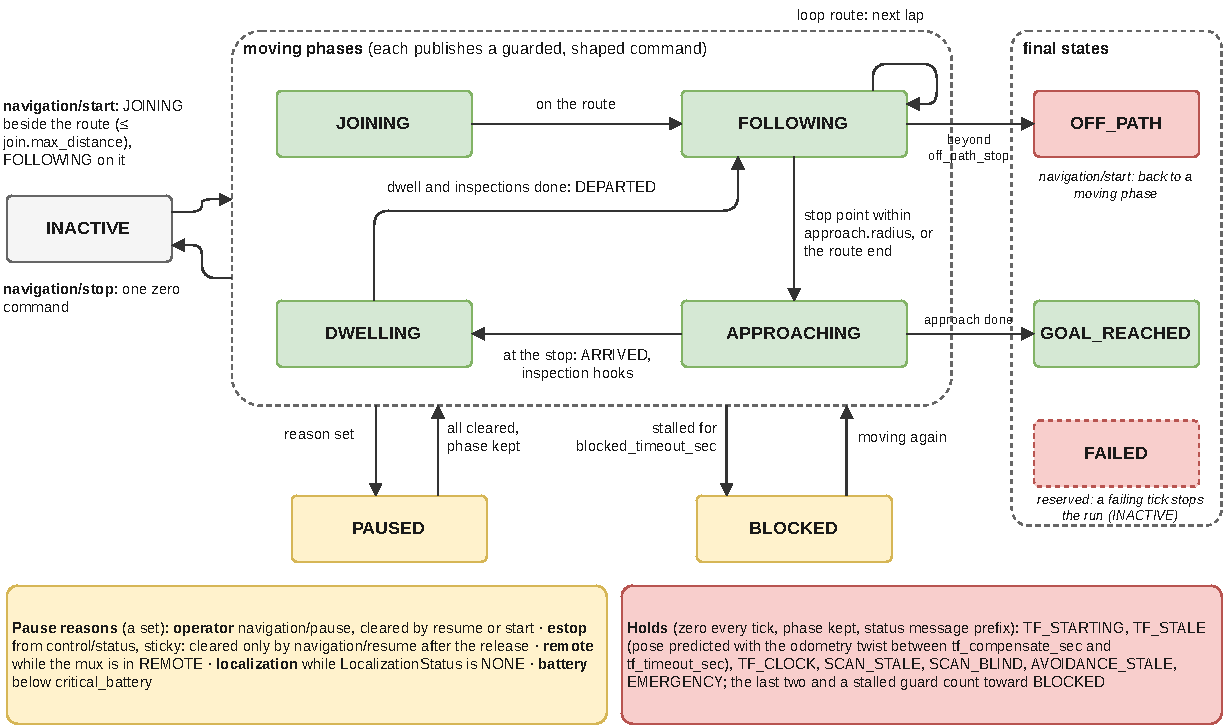
\includegraphics[width=\textwidth]{follower_fsm}
  \caption{States of the path follower, pause reasons and holds.}
  \label{fig:fsm}
\end{figure}

The follower is a pure state machine, \texttt{Follower.tick(inputs) -> Decision}: the node feeds it
the pose, the scans and the avoidance once per control tick and publishes the decision (command,
status, stop events). The states are the \code{NavigationStatus} constants and an explicit table
lists the allowed transitions (Fig.~\ref{fig:fsm}); a transition outside the table is a bug that
raises in the tests.

\subsection{Route, start and progress}

\topic{navigation/set_path} (planner) or the latched \topic{navigation/waypoints} (loader) give a
route of at least two points (review F17); a running follower starts over on a new route from
where the robot is. \topic{navigation/start} keeps the progress when the robot is still near it,
otherwise it locates the robot on the route, weighing the heading so the leg it walks along wins
over a parallel one. Beside the route (up to \param{join.max_distance}) it joins first
(\code{JOINING}); further away the start is refused. Start hooks (\param{hooks.start}) are called
asynchronously and the robot moves only when all succeeded.

Progress is searched in a short window ahead of the current one, against the line the robot is
meant to be on (route plus path offset), and its advance per tick is capped: a parallel leg never
captures it while the robot is shifted (review F5).

\subsection{Speed profile}

At each route point $i$ with curvature $\kappa_i$:
\begin{enumerate}
  \item curvature limit $v_i \le \sqrt{a_{\mathrm{lat}}/|\kappa_i|}$, clipped to
    $[v_{\min}, v_{\mathrm{cruise}}]$;
  \item approach speed at stop points and at the end;
  \item backward pass $v_i \le \sqrt{v_{i+1}^2 + 2 a_{\mathrm{dec}}\,\Delta s_i}$;
  \item the braking model \eqref{eq:m-braking}, reaction time included, before every stop;
  \item forward pass $v_{i+1} \le \sqrt{v_i^2 + 2 a_{\mathrm{acc}}\,\Delta s_i}$ out of the start
    and every stop (new in 0.2.0: the profile is consistent and predicts remaining time).
\end{enumerate}
Speeds and accelerations are capped by \param{robot.limits}. The speed regulator integrates a
signed error and resets on new paths; in 0.1 it integrated $|\omega| \ge 0$, so a positive gain
would have driven the speed to its minimum on long routes (finding N2).

\subsection{Controllers}

Controllers implement \code{PathController} and register in the \code{dharma.controllers}
registry; their parameters appear as \code{<name>.*} on the follower. Every controller applies
the avoidance the same way (finding N4): \code{heading_offset} (rad) rotates the commanded
direction of travel, \code{yaw_rate_bias} (rad/s) adds to the yaw rate.

\begin{center}
\begin{tabularx}{\textwidth}{@{}lX@{}}
  \toprule
  Controller & Law \\
  \midrule
  \code{holonomic} (default) & translation toward a carrot at arc length $s + L$ with
    $v = \min(v^*, \|\vect{c} - \vect{p}\|)$; heading toward the route direction a
    \code{heading_lookahead} ahead with a proportional, saturated yaw rate. The cross-track
    error obeys $\dot e = -v\,e/\sqrt{L^2 + e^2} \approx -(v/L)\,e$, so
    $e(t) = e_0 e^{-t/\tau}$ with $\tau = L/v$: 95\,\% after $3L$ of travel, independent of the
    speed. Lateral and heading loops are decoupled, which is why it does not oscillate on legged
    robots. \\
  \code{pure_pursuit}~\cite{coulter1992purepursuit} & curvature $2y/d^2$ toward the carrot at
    the requested speed \\
  \code{pid} & PID on the heading error toward the carrot, with a clamped integral
    (anti-windup, finding N2) \\
  \code{lqr} & error model $\vect{x} = [e_y, e_\psi]^\top$,
    $\vect{x}_{k+1} = \left[\begin{smallmatrix}1 & v\Delta t\\ 0 & 1\end{smallmatrix}\right]\vect{x}_k +
    \left[\begin{smallmatrix}0\\ \Delta t\end{smallmatrix}\right]u_k$, gain from the discrete Riccati
    equation per speed, $\omega = v\kappa - K\vect{x}$ \\
  \code{stanley}~\cite{thrun2006stanley} & $\omega = v\kappa - k_h\big(e_\psi +
    \arctan\frac{k\,e}{v + k_s}\big)$ toward the offset route \\
  \code{mppi}~\cite{williams2017mppi} & sampled yaw-rate sequences around the previous plan
    (warm start), unicycle rollouts, cost from route distance, carrot distance, intrusion into
    the clearance around the safety-scan points and effort, average $\vect{u}^* = \sum_i w_i
    \vect{u}_i$ with $w_i \propto \exp(-(J_i - J_{\min})/\lambda)$; seeded RNG (finding N2) \\
  \bottomrule
\end{tabularx}
\end{center}

\subsection{Path shift}

With \param{avoidance_mode} \code{path_shift} (omnidirectional robots), obstacle points of the
360° safety scan are expressed in route (Frenet) coordinates $(s, d)$~\cite{werling2010frenet}:
arc length along the route and signed distance to its left. A lateral offset $o$ is clear when no
point lies in the corridor
\begin{equation}
  |d - o| < w + c, \qquad s_{\mathrm{robot}} - b \le s \le s_{\mathrm{robot}} + f + \ell,
\end{equation}
($w$ half width, $c$ clearance, $b$, $f$ rear and front of the footprint, $\ell$ look-ahead).
Points beside the body block an offset outright; points ahead limit how far the robot can drive.
Among the candidates $o \in \{-o_{\max}, \ldots, o_{\max}\}$,
\begin{equation}
  o^* = \arg\min_{o\ \text{clear}}\ |o| + \lambda\,|o - o_{\mathrm{prev}}|,
\end{equation}
with a switch margin for other offsets than the current one; a move back toward the route is
taken only after it stayed proposed for \param{path_shift.return_delay_sec}. Without a clear
offset the robot keeps the one with the largest free distance (nearest the current one on ties)
and slows. The commanded offset moves toward the target at \param{path_shift.offset_rate}. The
speed limit is $v^*(d_{\mathrm{free}} - m)$ where $d_{\mathrm{free}}$ is the smallest free
distance over the target offset, the commanded offset \emph{and the measured lateral offset}
(review F4), so a robot still sliding is not sped up by the offset it has not reached. A blind
scan stops the robot. Near a stop point it stays on the route and waits for an obstacle instead
of passing it (review F6).

\subsection{Reactive avoidance}

With \code{reactive}, \code{obstacle_avoidance_node} runs one policy of the
\code{dharma.avoidance} registry on \topic{perception/sector_scan} and publishes an
\code{AvoidanceCommand}: heading offset (rad), yaw-rate bias (rad/s), lateral bias (m/s, omni),
speed scale and an emergency flag (an obstacle closer than \param{shared.emergency_distance} in
the cone $\pm$\param{shared.emergency_cone_deg}). Blocked sectors are obstacles.
\begin{center}
\begin{tabularx}{\textwidth}{@{}lX@{}}
  \toprule
  Policy & Principle \\
  \midrule
  \code{braitenberg} & danger left and right steers, danger ahead or beside slows \\
  \code{vfh}~\cite{borenstein1991vfh} (default) & only when the frontal cone is blocked, aim at
    the nearest edge of a wide enough gap \\
  \code{potential_field}~\cite{khatib1986potential} & obstacles inside the safe distance repel,
    $\vect{F} = -\sum_j \eta\big(\tfrac{1}{r_j} - \tfrac{1}{r_0}\big)\tfrac{1}{r_j^2}\hat{\vect{u}}_j$;
    the sideways part steers and pushes, danger ahead slows \\
  \code{follow_gap}~\cite{sezer2012ftg} & bubble the nearest obstacle, aim at the centre of the
    widest gap \\
  \bottomrule
\end{tabularx}
\end{center}
The outputs are smoothed asymmetrically: the speed scale drops at once and only rises through
the filter, the emergency flag is never filtered (review F13).

\textbf{Is the emergency cone enough?} With $\tr = 0.25$~s the stopping distances are
\begin{center}
\begin{tabular}{@{}lrrl@{}}
  \toprule
  $v$ & $a = 0.5$ & $a = 0.6$ & 0.35~m of room? \\
  \midrule
  0.35~m/s (cruise in 0.1) & 0.21~m & 0.19~m & yes \\
  0.60~m/s & 0.51~m & 0.45~m & no \\
  1.0~m/s & 1.25~m & 1.08~m & no \\
  \bottomrule
\end{tabular}
\end{center}
so the cone (0.75~m from \frm{base_link}, about 0.35~m from the nose) is a second line; the motion
guard and the protective field limit the speed before.

\subsection{Stop points}

Stop points (\texttt{dwell\_sec > 0}) are detected by progress (within \param{approach.radius} along
the route) and by distance minus the path offset; a stop on a later leg that passes close never
triggers early, and one is skipped only once the progress passed it by
\param{approach.skip_margin} (review F6). At a stop: final x, y, yaw approach, \code{ARRIVED},
inspection hooks (asynchronous; answers for an earlier stop or route are dropped), dwell,
\code{DEPARTED}. Route processing keeps stop points closer than 3~cm apart (review F12).

\subsection{Supervisor, motion guard and command shaper}

\begin{itemize}
  \item \textbf{Pose.} \code{TF_STARTING} without a pose; \code{TF_STALE} above
    \param{safety.tf_timeout_sec}; between \param{safety.tf_compensate_sec} and the timeout the
    pose is predicted forward with the odometry twist instead of stopping; \code{TF_CLOCK} for a
    pose from the future (clock mismatch).
  \item \textbf{Scans and avoidance.} \code{SCAN_STALE}, \code{SCAN_BLIND} (blocked sectors),
    \code{AVOIDANCE_STALE}, \code{EMERGENCY} (held for \param{safety.emergency_release_sec}).
  \item \textbf{Blocked and off path.} No progress for \param{safety.blocked_timeout_sec} is
    \code{BLOCKED}; more than \param{safety.off_path_stop} from the route beyond the path offset is
    \code{OFF_PATH} (the robot slows from \param{safety.off_path_slow}).
  \item \textbf{Motion guard.} Every command, in every phase (following, joining, final
    approach), is limited along its direction by the 360° safety scan with the footprint and the
    braking model, and the yaw rate by the free turning angle (review F7; 0.1 checked joining
    and the final approach with the front cone only).
  \item \textbf{Command shaper.} Robot envelope (x and y scaled together, $v_y = 0$ for diff
    robots), smoothing of yaw rate and sideways speed, slew limits from \param{robot.limits},
    non-finite values to zero (review F11).
\end{itemize}
Zero commands are published once on entering \code{INACTIVE} or a final state, every tick while
paused or held, on stop, on shutdown (a hook) and when a control tick raises (review F2). All
state-changing callbacks and the control loop share one mutually exclusive callback group and a
lock (review F3); timers (dwell, approach) are frozen while paused (review F7).

\subsection{Pause reasons}

A set of reasons, each with its own way of clearing (review F16):
\begin{center}
\begin{tabularx}{\textwidth}{@{}lX@{}}
  \toprule
  Reason & Set and cleared \\
  \midrule
  \code{operator} & \topic{navigation/pause}; cleared by \topic{navigation/resume} or start \\
  \code{estop} & \topic{control/status} reports the e-stop; sticky: cleared only by
    \topic{navigation/resume} after the release, so the robot never drives off on its own after
    an e-stop \\
  \code{remote} & while the mux is in REMOTE \\
  \code{localization} & while \topic{localization/status} is \code{NONE}; cleared when localized
    again \\
  \code{battery} & below \param{critical_battery}; below \param{low_battery} a loop route finishes
    its lap and stops \\
  \bottomrule
\end{tabularx}
\end{center}
Start is refused while \code{estop} or \code{localization} hold.

\section{Interfaces}

\begin{center}
\begin{tabularx}{\textwidth}{@{}p{0.36\textwidth}p{0.24\textwidth}X@{}}
  \toprule
  Interface & Type & \\
  \midrule
  \topic{planner/go_to}, \topic{planner/plan} & GoTo, PlanPath & plan (and drive) to x, y, yaw \\
  \topic{planner/cancel} & Trigger & \\
  \topic{planner/status}, \topic{planner/path}, \topic{planner/costmap} & PlannerStatus, Path,
    OccupancyGrid & latched \\
  \topic{navigation/set_path}, \topic{navigation/load_path} & SetPath, LoadPath & \\
  \topic{navigation/start}, \topic{stop}, \topic{pause}, \topic{resume} & Trigger & \\
  \topic{navigation/status} & NavigationStatus, latched & state, pause reasons, progress \\
  \topic{navigation/stop_point} & StopPointEvent & \\
  \topic{navigation/waypoints}, \topic{navigation/path} & WaypointPath, Path & loaded route \\
  \topic{navigation/avoidance} & AvoidanceCommand & avoidance $\to$ follower \\
  \topic{control/nav_cmd_vel} & Twist & to the control mux \\
  in: \topic{/map}, \topic{perception/safety_scan}, \topic{perception/sector_scan},
    \topic{control/status}, \topic{localization/status}, battery, odom & & \\
  \bottomrule
\end{tabularx}
\end{center}

\section{Parameters}

\readonlynote

% Generated by docs/manual/tools/reference.py; do not edit.
\begin{small}
\begin{longtable}{@{}>{\raggedright}p{0.25\textwidth}>{\raggedright}p{0.17\textwidth}>{\raggedright}p{0.10\textwidth}>{\raggedright}p{0.11\textwidth}>{\raggedright\arraybackslash}p{0.25\textwidth}@{}}
\toprule
Parameter & Default & Unit & Range & Description \\
\midrule
\endhead
\bottomrule
\endfoot
\multicolumn{5}{@{}l}{\textbf{planner\_\allowbreak{}node}} \\
\code{costmap.resolution} & 0.1 & m & 0.01..1 & planning cell size, the map is max-pooled to it \\
\code{costmap.margin} & 0.1 & m & 0..1 & clearance added to the footprint (keep >= half a cell) \\
\code{costmap.inflation_radius} & 0.8 & m & 0..5 & paths keep away from walls up to here \\
\code{costmap.cost_scaling} & 3 & 1/\allowbreak{}m & 0..50 & how fast the wall cost falls off \\
\code{costmap.unknown_is_obstacle} & true &  &  & never plan through unmapped space \\
\code{costmap.occupied_threshold} & 50 &  & 1..100 & map values from here are obstacles \\
\code{search.goal_tolerance} & 0.5 & m & 0..5 & a goal in an obstacle moves to free space this close \\
\code{search.start_escape} & 1 & m & 0..5 & a robot inside the inflation walks out up to here \\
\code{search.heuristic_weight} & 1 &  & 1..5 & > 1: faster search, slightly longer paths \\
\code{search.timeout_sec} & 5 & s & 0.1..60 & search time limit \\
\code{search.spacing} & 0.1 & m & 0.02..1 & distance between waypoints \\
\code{search.smooth_weight_data} & 0.1 &  & 0..1 & pull toward the search path \\
\code{search.smooth_weight_smooth} & 0.3 &  & 0..0.49 & pull toward the neighbours \\
\code{search.footprint_retries} & 5 &  & 0..20 & searches around poses where the oriented footprint collides \\
\code{monitor.arrival_tolerance} & 0.35 & m & 0.01..5 & GOAL\_\allowbreak{}REACHED counts this close to the plan goal \\
\code{monitor.stop_on_arrival} & true &  &  & stop the follower at the goal \\
\code{monitor.replan_after_sec} & 3 & s & 0.1..300 & follower BLOCKED this long: plan again \\
\code{monitor.max_replans} & 5 &  & 0..100 & per goal, then failed \\
\code{monitor.cancel_after_sec} & 1 & s & 0.1..60 & follower INACTIVE this long: cancelled \\
\code{use_live_obstacles} & true &  &  & replans see the obstacles of the safety scan \\
\code{scan_timeout_sec}$^\dagger$ & 1 & s & 0.05..10 & older safety scans are ignored \\
\code{tf_timeout_sec}$^\dagger$ & 0.5 & s & 0.05..10 & an older robot pose is unknown \\
\code{publish_costmap} & false &  &  & planner/costmap for RViz (debug) \\
\code{status_hz} & 2 & Hz & 0.1..50 & planner/status while active \\
\code{service_timeout_sec} & 5 & s & 0.1..60 & calls to the follower \\
\multicolumn{5}{@{}l}{\textbf{path\_\allowbreak{}loader\_\allowbreak{}node}} \\
\code{sites_dir}$^\dagger$ & \code{~/dharma/map} &  &  & routes are loaded from inside this directory only \\
\code{route}$^\dagger$ & \code{""} &  &  & route CSV loaded at start (inside sites\_\allowbreak{}dir) \\
\code{remember_file}$^\dagger$ & \code{~/.dharma/last_route} &  &  & last loaded route, reloaded at start ("": off) \\
\code{process} & true &  &  & resample and smooth routes between stop points \\
\code{processing.spacing} & 0.1 & m & 0.02..1 & point spacing after resampling \\
\code{processing.smooth_weight_data} & 0.05 &  & 0..1 & pull toward the recording \\
\code{processing.smooth_weight_smooth} & 0.4 &  & 0..0.49 & pull toward neighbours \\
\code{processing.max_deviation} & 0.3 & m & 0..5 & warn when smoothing moves the route further \\
\code{republish_sec} & 2 & s & 0..60 & navigation/path republish for RViz (0: off) \\
\multicolumn{5}{@{}l}{\textbf{path\_\allowbreak{}follower\_\allowbreak{}node}} \\
\code{control_rate}$^\dagger$ & 20 & Hz & 1..200 & loop rate \\
\code{controller} & \code{holonomic} &  &  & path controller (dharma.controllers) \\
\code{avoidance_mode} & \code{path_shift} &  & path\_\allowbreak{}shift, reactive, off & path\_\allowbreak{}shift: slide sideways (holonomic) \\
\code{loop_route} & false &  &  & restart a closed route at its end (patrol) \\
\code{loop_close_distance} & 1 & m & 0..20 & end this close to the start: a closed route \\
\code{require_localization} & true &  &  & pause while localization/status is NONE \\
\code{low_battery} & 0.2 &  & 0..1 & below: finish the lap, no new one \\
\code{critical_battery} & 0.1 &  & 0..1 & below: pause (reason battery) \\
\code{battery_hysteresis} & 0.05 &  & 0..0.5 & recharge above + this \\
\code{speed.cruise} & 0.4 & m/\allowbreak{}s & 0.01..5 & cruise speed \\
\code{speed.min_speed} & 0.1 & m/\allowbreak{}s & 0..5 & floor of the curve limit \\
\code{speed.approach_speed} & 0.15 & m/\allowbreak{}s & 0.01..5 & speed at stop points and the route end \\
\code{speed.lateral_accel} & 0.3 & m/\allowbreak{}s$^{2}$ & 0.01..10 & curve limit v = sqrt(a / curvature) \\
\code{speed.accel} & 0.3 & m/\allowbreak{}s$^{2}$ & 0.01..20 & comfortable acceleration \\
\code{speed.decel} & 0.3 & m/\allowbreak{}s$^{2}$ & 0.01..20 & comfortable braking \\
\code{speed.smoothing} & 0.5 &  & 0.05..1 & weight of a new yaw rate / sideways command (1: off) \\
\code{safety.stop_margin}$^\dagger$ & 0.3 & m & 0..5 & gap kept to obstacles when stopping \\
\code{safety.yaw_margin_deg}$^\dagger$ & 5 & deg & 0..90 & turning room kept to obstacles \\
\code{safety.scan_timeout_sec}$^\dagger$ & 0.5 & s & 0.05..5 & older safety scans stop the robot \\
\code{safety.avoidance_timeout_sec}$^\dagger$ & 0.5 & s & 0.05..5 & older avoidance (reactive) stops it \\
\code{safety.tf_timeout_sec}$^\dagger$ & 0.5 & s & 0.05..5 & an older pose stops the robot \\
\code{safety.tf_compensate_sec}$^\dagger$ & 0.1 & s & 0..5 & older poses are predicted forward \\
\code{safety.clock_tolerance_sec}$^\dagger$ & 0.1 & s & 0..5 & a pose from further in the future: clock \\
\code{safety.emergency_release_sec} & 1 & s & 0..30 & an emergency stop holds this long after it clears \\
\code{safety.blocked_timeout_sec} & 10 & s & 0.5..600 & no progress this long: BLOCKED \\
\code{safety.off_path_slow} & 0.6 & m & 0.05..10 & further from the route: slow to the floor speed \\
\code{safety.off_path_stop} & 1.5 & m & 0.1..20 & further from the route: OFF\_\allowbreak{}PATH, stopped \\
\code{path_shift.max_offset} & 0.8 & m & 0..5 & furthest from the route \\
\code{path_shift.step} & 0.1 & m & 0.02..1 & candidate offset spacing \\
\code{path_shift.look_ahead} & 2 & m & 0.1..20 & route ahead of the front edge that must be free \\
\code{path_shift.clearance} & 0.1 & m & 0..2 & gap kept beside the body \\
\code{path_shift.offset_rate} & 0.3 & m/\allowbreak{}s & 0.01..5 & how fast it slides onto a new offset \\
\code{path_shift.switch_cost} & 0.5 &  & 0..10 & keeps its side (hysteresis) \\
\code{path_shift.switch_margin} & 0.05 & m & 0..1 & extra clearance a new offset needs \\
\code{path_shift.return_delay_sec} & 0.5 & s & 0..30 & a way back must stay proposed this long \\
\code{path_shift.stop_margin} & 0.4 & m & 0..5 & stop this far before an obstacle (front edge) \\
\code{approach.radius} & 0.5 & m & 0.05..5 & this close (along the route) the approach starts \\
\code{approach.skip_margin} & 0.5 & m & 0.05..10 & progress this far past a stop: skipped \\
\code{approach.timeout_sec} & 20 & s & 1..600 & give up converging (paused time not counted) \\
\code{approach.kp_xy} & 1.2 & 1/\allowbreak{}s & 0..10 & gain on the position error \\
\code{approach.kp_yaw} & 1.5 & 1/\allowbreak{}s & 0..10 & gain on the yaw error \\
\code{approach.max_speed} & 0.2 & m/\allowbreak{}s & 0.01..2 & approach speed cap \\
\code{approach.max_yaw_rate} & 0.6 & rad/\allowbreak{}s & 0.01..5 & yaw rate cap \\
\code{approach.min_speed} & 0.04 & m/\allowbreak{}s & 0..1 & floor to beat the robot deadband \\
\code{approach.position_tolerance} & 0.05 & m & 0.005..1 & arrived within \\
\code{approach.yaw_tolerance_deg} & 3 & deg & 0.1..45 & aligned within \\
\code{join.max_distance} & 3 & m & 0..50 & a robot this far walks onto the route (0: off) \\
\code{join.timeout_sec} & 60 & s & 1..600 & give up and follow from where it is \\
\code{join.on_route} & 0.15 & m & 0.01..2 & joined within this \\
\code{hooks.start}$^\dagger$ & [] &  &  & called on start; the robot waits for every success \\
\code{hooks.stop}$^\dagger$ & [] &  &  & called on stop (not waited for) \\
\code{hooks.inspection}$^\dagger$ & [] &  &  & called at every stop point \\
\code{hooks.timeout_sec}$^\dagger$ & 5 & s & 0.1..120 & start and stop hook timeout \\
\code{hooks.inspection_timeout_sec} & 20 & s & 0.1..600 & a stop waits this long for inspections \\
\code{regulator.enabled} & false &  &  & scale the speed down when turning hard \\
\code{regulator.reference_yaw_rate} & 0.3 & rad/\allowbreak{}s & 0..5 & turning slower than this needs no slow-down \\
\code{regulator.kp} & 0.5 & s/\allowbreak{}rad & 0..10 & scale per rad/s above it \\
\code{regulator.ki} & 0 & 1/\allowbreak{}rad & 0..10 & scale per integrated rad \\
\code{regulator.integral_limit} & 1 & rad & 0..10 & anti-windup clamp \\
\code{regulator.min_scale} & 0.3 &  & 0..1 & never slower than this fraction \\
\code{processing.spacing} & 0.1 & m & 0.02..1 & point spacing after resampling \\
\code{processing.smooth_weight_data} & 0.05 &  & 0..1 & pull toward the recording \\
\code{processing.smooth_weight_smooth} & 0.4 &  & 0..0.49 & pull toward neighbours \\
\code{processing.max_deviation} & 0.3 & m & 0..5 & warn when smoothing moves the route further \\
\code{markers} & true &  &  & publish RViz markers \\
\multicolumn{5}{@{}l}{\textbf{obstacle\_\allowbreak{}avoidance\_\allowbreak{}node}} \\
\code{policy} & \code{vfh} &  &  & avoidance policy (dharma.avoidance) \\
\code{shared.safe_distance} & 1 & m & 0.1..20 & obstacles closer than this shape the command \\
\code{shared.emergency_distance} & 0.75 & m & 0..10 & obstacle in the cone closer than this: stop \\
\code{shared.emergency_cone_deg} & 60 & deg & 1..360 & frontal cone of the emergency stop \\
\code{shared.max_heading_offset_deg} & 60 & deg & 0..180 & largest turn of the direction of travel \\
\code{shared.smoothing} & 0.8 &  & 0..0.99 & 0..1 filter on steering and speeding up (never on braking) \\
\code{braitenberg.steering_gain} & 1 & rad & 0..10 & turn per unit danger \\
\code{braitenberg.velocity_gain} & 1 &  & 0..10 & slow-down per unit danger \\
\code{braitenberg.steering_zone_center_deg} & 45 & deg & 0..180 &  \\
\code{braitenberg.steering_zone_width_deg} & 60 & deg & 1..360 &  \\
\code{braitenberg.velocity_zone_center_deg} & 60 & deg & 0..180 &  \\
\code{braitenberg.velocity_zone_width_deg} & 90 & deg & 1..360 &  \\
\code{braitenberg.following_zone_width_deg} & 30 & deg & 1..360 &  \\
\code{vfh.min_gap_width_deg} & 20 & deg & 1..180 & narrowest passable gap \\
\code{vfh.steering_gain} & 1 &  & 0..5 & fraction of the gap heading taken \\
\code{vfh.velocity_gain} & 1 &  & 0..10 & slow-down per unit frontal danger \\
\code{potential_field.repulsion_gain} & 0.5 &  & 0..10 & strength of the repulsion \\
\code{potential_field.steering_gain} & 0.8 & rad & 0..5 & turn per atan(force) \\
\code{potential_field.lateral_gain} & 0.3 &  & 0..5 & sideways m/s per unit force \\
\code{potential_field.max_lateral} & 0.2 & m/\allowbreak{}s & 0..2 & cap on the sideways push \\
\code{potential_field.velocity_gain} & 1 &  & 0..10 & slow-down per unit frontal danger \\
\code{follow_gap.bubble_radius} & 0.45 & m & 0..5 & safety bubble around the nearest obstacle \\
\code{follow_gap.steering_gain} & 1 &  & 0..5 & fraction of the gap heading taken \\
\code{follow_gap.velocity_gain} & 1 &  & 0..10 & slow-down per unit frontal danger \\
\code{markers} & true &  &  & publish RViz markers \\
\end{longtable}
\end{small}


\subsection{Controller parameters}

% Generated by docs/manual/tools/reference.py; do not edit.
\begin{small}
\begin{longtable}{@{}p{0.28\textwidth}p{0.12\textwidth}p{0.08\textwidth}p{0.11\textwidth}p{0.29\textwidth}@{}}
\toprule
Parameter & Default & Unit & Range & Description \\
\midrule
\endhead
\bottomrule
\endfoot
\multicolumn{5}{@{}l}{\textbf{path\_follower\_node: holonomic}} \\
\code{holonomic.lookahead} & 0.6 & m & 0.1\,..\,5 & carrot ahead along the route; longer = gentler \\
\code{holonomic.heading_lookahead} & 0.6 & m & 0.1\,..\,5 & the heading follows the route this far ahead \\
\code{holonomic.kp_yaw} & 1.5 & 1/s & 0\,..\,10 & yaw rate per rad of error \\
\code{holonomic.max_lateral_speed} & 0.25 & m/s & 0\,..\,5 & sideways speed cap (0: never strafe) \\
\code{holonomic.max_reverse_speed} & 0.15 & m/s & 0\,..\,5 & backward speed cap when the route is behind \\
\code{holonomic.min_alignment_scale} & 0.25 &  & 0\,..\,1 & translation factor while the heading is far off \\
\multicolumn{5}{@{}l}{\textbf{path\_follower\_node: pure\_pursuit}} \\
\code{pure_pursuit.lookahead} & 1 & m & 0.1\,..\,5 & carrot ahead along the route \\
\multicolumn{5}{@{}l}{\textbf{path\_follower\_node: pid}} \\
\code{pid.lookahead} & 1 & m & 0.1\,..\,5 & carrot ahead along the route \\
\code{pid.kp} & 1.5 & 1/s & 0\,..\,20 & proportional gain \\
\code{pid.ki} & 0 & 1/s$^{2}$ & 0\,..\,20 & integral gain \\
\code{pid.kd} & 0.2 &  & 0\,..\,20 & derivative gain \\
\code{pid.integral_limit} & 0.5 & rad s & 0\,..\,10 & anti-windup clamp of the error integral \\
\multicolumn{5}{@{}l}{\textbf{path\_follower\_node: lqr}} \\
\code{lqr.q_lateral} & 1 &  & 0\,..\,100 & weight on the cross-track error \\
\code{lqr.q_heading} & 0.5 &  & 0\,..\,100 & weight on the heading error \\
\code{lqr.r_yaw_rate} & 0.5 &  & 0.001\,..\,100 & weight on the yaw rate (higher = gentler) \\
\multicolumn{5}{@{}l}{\textbf{path\_follower\_node: stanley}} \\
\code{stanley.k_cross_track} & 1 &  & 0\,..\,20 & cross-track gain \\
\code{stanley.k_soft} & 0.2 & m/s & 0.01\,..\,5 & softening so low speeds do not over-steer \\
\code{stanley.k_heading} & 1.5 & 1/s & 0\,..\,20 & steering to yaw rate gain \\
\multicolumn{5}{@{}l}{\textbf{path\_follower\_node: mppi}} \\
\code{mppi.horizon_steps} & 15 &  & 2\,..\,100 & steps per rollout \\
\code{mppi.step_sec} & 0.1 & s & 0.01\,..\,1 & rollout step \\
\code{mppi.samples} & 200 &  & 10\,..\,5000 & rollouts per tick \\
\code{mppi.yaw_rate_std} & 1 & rad/s & 0.01\,..\,5 & sampling noise \\
\code{mppi.temperature} & 0.05 &  & 0.001\,..\,100 & softmax sharpness of the normalized cost \\
\code{mppi.window} & 4 & m & 0.5\,..\,20 & route ahead in the cost \\
\code{mppi.obstacle_weight} & 5 &  & 0\,..\,1000 & cost per m of intrusion \\
\code{mppi.clearance} & 0.5 & m & 0\,..\,5 & rollouts closer to an obstacle pay for it \\
\code{mppi.seed}$^\dagger$ & 0 &  & 0\,..\,2.14748e+09 & random seed (reproducible) \\
\end{longtable}
\end{small}


\chapter{Control and safety}
\label{ch:control}

\pkg{dharma_control} contains \code{control_mux_node}, the \textbf{only} publisher of the
robot's \topic{cmd_vel}. It arbitrates navigation (AUTO) and one operator source (REMOTE), keeps
every command inside the robot's envelope, limits it with a protective field on the 360° safety
scan and holds a latched e-stop with a hardware input and re-arm.

\begin{figure}[h]
  \centering
  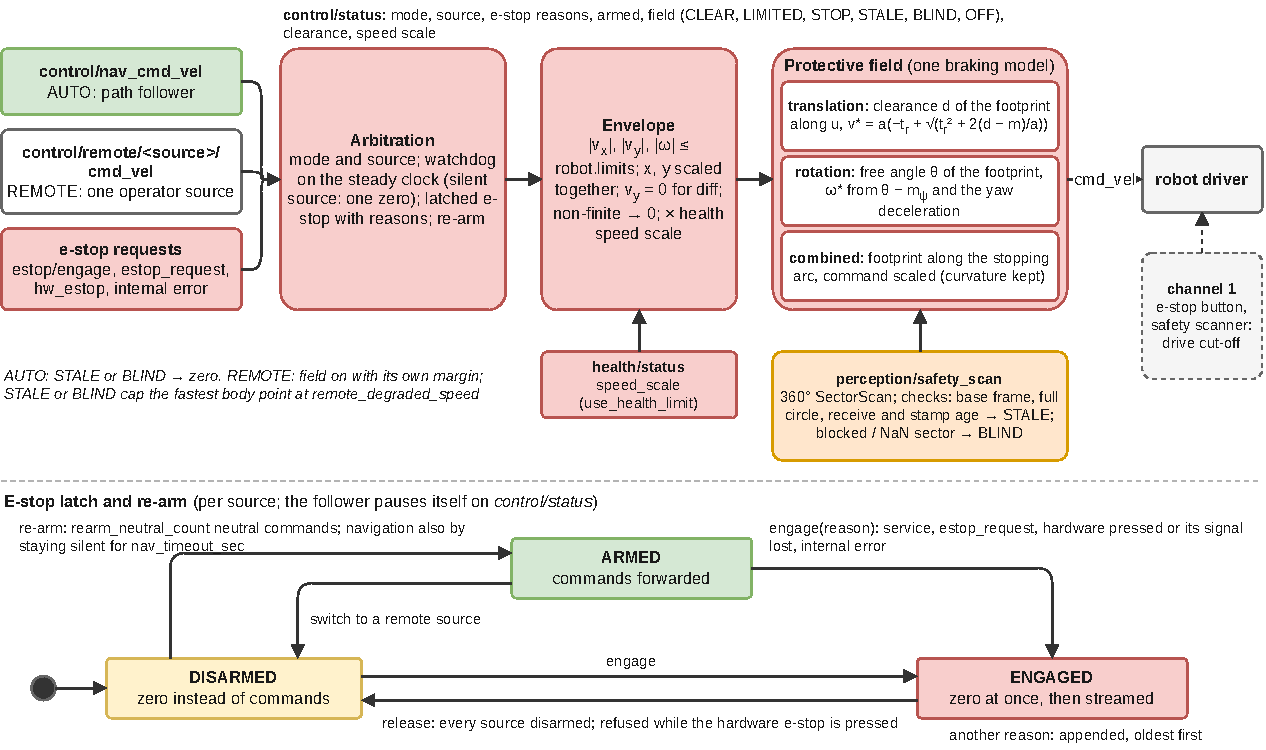
\includegraphics[width=\textwidth]{safety_pipeline}
  \caption{The safety layer and the e-stop latch with re-arm.}
  \label{fig:m-safety}
\end{figure}

\section{Two-channel safety architecture}
\label{sec:two-channel}

The control mux is a software safety function in Python over DDS. It is \emph{not} certified and
must never be the only protection of a robot that drives among people (finding C2). Products for
public spaces use two channels:

\begin{center}
\begin{tabularx}{\textwidth}{@{}p{0.18\textwidth}Xp{0.27\textwidth}@{}}
  \toprule
  Channel & What & Stops the robot by \\
  \midrule
  1 (hardware) & e-stop buttons and, where required, a safety-rated scanner or bumper wired to
    the drive's safe torque off or brake input, designed to ISO 13849-1~\cite{iso13849} (for
    example PL~d) or IEC 61508~\cite{iec61508}; ISO 13482~\cite{iso13482} applies to personal
    care robots & cutting the drive, independently of any software \\
  2 (\code{control_mux_node}) & envelope, protective field, watchdogs, latched software e-stop:
    smooth, early, configurable & publishing zero on \topic{cmd_vel} and streaming zero while
    engaged \\
  \bottomrule
\end{tabularx}
\end{center}

Wire channel~1's state to \topic{control/hw_estop} (Bool, true = pressed): while it is pressed
the software e-stop cannot be released, and after the button is released an operator still has
to release the software e-stop explicitly. With \param{hw_estop_timeout_sec} $> 0$ a silent
publisher of \topic{control/hw_estop} engages the e-stop (the signal is then required). The
driver must stop on its own command timeout, which covers a crash of the mux until it respawns.

\section{Pipeline}

\subsection{Arbitration}

AUTO forwards \topic{control/nav_cmd_vel}; REMOTE forwards
\topic{control/remote/<source>/cmd_vel} of the selected source only (\param{remote_sources},
default \texttt{[handheld, dashboard]}; review \#8: several operators on one topic).
\topic{control/set_mode} with the current mode and source is a no-op (review \#13); a change
publishes one zero and resets the watchdog; unknown modes or sources are rejected. The
\textbf{watchdog} gives the active source one zero when it is silent longer than
\param{nav_timeout_sec} or \param{remote_timeout_sec}. All timeouts and the e-stop hold run on the
steady clock: clock jumps and \code{use_sim_time} never disable them (review \#4).

\subsection{E-stop latch and re-arm}

\begin{itemize}
  \item \textbf{Engage.} \topic{control/estop/engage} (Trigger), \topic{control/estop_request}
    (String reason), \topic{control/hw_estop}, a silent hardware signal, or an internal error.
    Reasons accumulate, oldest first, without duplicates (review \#14). Zero is published at once
    and streamed at \param{estop_hold_hz}. Mode switches are allowed while engaged but forward
    nothing.
  \item \textbf{Release.} \topic{control/estop/release} (Trigger) is refused while the hardware
    e-stop is pressed; it clears the reasons and disarms every source. There is no
    \code{SetBool}: in 0.1 a default request released the e-stop and anyone could release
    anyone's e-stop (review \#3).
  \item \textbf{Re-arm.} At start, after a release and after switching to a remote source, a
    source is disarmed: it must send \param{rearm_neutral_count} consecutive neutral commands
    (every axis below \param{neutral_eps}) before anything it sends is forwarded, so a stick held
    during a release never moves the robot (review B3). Navigation also re-arms by staying silent
    for \param{nav_timeout_sec}.
  \item \textbf{Navigation pauses itself.} The mux never calls navigation services (review B3:
    the e-stop was resumed through \code{set_mode}); the follower reads \topic{control/status}:
    \code{estop} is a sticky pause reason there (cleared by \topic{navigation/resume}),
    \code{remote} a transient one.
\end{itemize}

\subsection{Envelope}

$|v_x| \le$ \param{max_vx}, $|v_y| \le$ \param{max_vy} (0 for \code{diff}), $|\omega| \le$
\param{max_wz} from \param{robot.limits}; $v_x$ and $v_y$ are scaled together, keeping the
direction. Any non-finite axis makes the command zero (review \#5: NaN limits disabled the
envelope). With \param{use_health_limit}, every axis is multiplied by \code{HealthStatus.speed_scale}
(stale health: no change). Commands are clamped before the field.

\subsection{Protective field}

AUTO always; REMOTE when \param{field.in_remote} (default true since 0.2.0, with
\param{field.remote_margin}). The model is speed and separation
monitoring~\cite{isots15066,marvel2016ssm} with the braking model of
Section~\ref{sec:braking}.

\textbf{Translation.} For the commanded direction $\hat{\vect{u}}$, the clearance $d_t$ is the
distance the footprint can move before touching a scan point
(\code{translation_clearance}): points ahead of the leading edge count when they lie within the
body corridor widened by \param{field.lateral_margin}; a point beside the body (behind the
leading edge, inside the corridor) or inside the footprint gives 0. The speed is limited to
$v^*(d_t - m)$ with $m$ = \param{field.margin}; below \param{field.min_speed} it stops. With
$a = 0.6$~m/s$^2$, $\tr = 0.25$~s and $m = 0.15$~m:
\begin{center}
\begin{tabular}{@{}lrrrr@{}}
  \toprule
  free distance $d_t$ & 0.3~m & 0.5~m & 1.0~m & 2.0~m \\
  allowed speed $v^*$ & 0.30~m/s & 0.52~m/s & 0.87~m/s & 1.35~m/s \\
  \bottomrule
\end{tabular}
\end{center}

\textbf{Rotation} (finding C1). In 0.1 only $v_x, v_y$ were scaled: a pure rotation passed
unchecked, although the corners of the footprint sweep the ring $r_{\mathrm{in}} < r \le
r_{\mathrm{c}}$ (0.28 to 0.49~m) and hit obstacles beside the robot. Now the free angle
$\theta_f$ (\code{rotation_room}: the ring points are rotated in 1° steps against the turning
direction until one enters the footprint; a point already inside gives 0) bounds the yaw rate:
$|\omega| \le \omega^*(\theta_f - m_\psi)$ with the yaw deceleration \param{max_yaw_accel} and
$m_\psi$ = \param{field.yaw_margin}; below \param{field.min_yaw_rate} it stops.

\textbf{Combined motion.} For $(v_x, v_y, \omega)$ the robot keeps the twist for $\tr$ and then
brakes both axes in proportion (the arc is kept) over $T_b = \max(v/a, |\omega|/\alpha)$. It covers
the constant-twist arc
\begin{equation}
  x(u) = \frac{v_x\sin\omega u - v_y(1 - \cos\omega u)}{\omega}, \quad
  y(u) = \frac{v_x(1 - \cos\omega u) + v_y\sin\omega u}{\omega}, \quad \psi(u) = \omega u
\end{equation}
up to $u = \tr + T_b/2$, exactly $D(v)$ on a straight line, plus an extension of
$\min(m/v, m_\psi/|\omega|)$. The footprint (widened by the lateral margin) is checked at poses
along the arc; a point already beside the body may be passed but not approached closer than
2~cm. If the first contact is at $u_c$, scaling by $s$ keeps the curvature and covers
$s\,\tr + s^2 T_b/2$, so the largest clear scale is
\begin{equation}
  s = \frac{-\tr + \sqrt{\tr^2 + 2\,T_b\,(u_c - u_{\mathrm{ext}})}}{T_b}.
\end{equation}

\subsection{Scan validation and degraded sensing}

\topic{perception/safety_scan} is accepted only in \param{robot.frames.base} with full-circle
coverage (review \#7). It is \code{STALE} when invalid, not received for
\param{field.scan_timeout_sec} (monotonic receive age) or when its stamp is older than
\param{field.scan_max_age_sec} or more than \param{field.scan_clock_tolerance_sec} in the future.
Any blocked or NaN sector makes it \code{BLIND} (review B1: an all-zero scan was read as clear).
\begin{itemize}
  \item AUTO: \code{STALE} or \code{BLIND} $\to$ zero; no scan at all $\to$ zero.
  \item REMOTE: the fastest point of the body ($v + |\omega| r_{\mathrm{c}}$) is capped at
    \param{field.remote_degraded_speed}; with a partly blind scan the field still applies to the
    points it sees, and a translation toward a blocked sector is refused.
\end{itemize}
\code{control/status} reports the field state (\code{CLEAR}, \code{LIMITED}, \code{STOP},
\code{STALE}, \code{BLIND}, \code{OFF}), the clearance and the applied speed scale.

\subsection{Fail-safe behaviour}

An exception in any callback engages the e-stop with the reason \texttt{internal error} and
publishes zero (review \#6); on shutdown the node publishes zero three times. Safety parameters
are read-only at runtime and validated at start (decelerations $> 0$, timeouts $> 0$, margins
$\ge 0$, finite values): the node refuses to start on a bad value (review \#5:
\texttt{max\_decel: 0} raised \code{ZeroDivisionError}).

\section{Safety case}
\label{sec:safety-case}

Hazards of the navigation function, their mitigations in the stack and the tests that verify
them. Test names are \code{file::function} in the package's \code{test/} directory (u: unit, r:
node test). The software mitigations are channel~2; residual risks need channel~1 or a sensor
the stack does not have.

\begin{small}
\begin{longtable}{@{}>{\raggedright}p{0.04\textwidth}>{\raggedright}p{0.25\textwidth}>{\raggedright}p{0.31\textwidth}>{\raggedright\arraybackslash}p{0.32\textwidth}@{}}
  \toprule
  & Hazard & Mitigation & Verification \\
  \midrule
  \endhead
  \bottomrule
  \endfoot
  H1 & collision with an obstacle ahead while driving & protective field translation limit
    with one braking model; follower motion guard; speed profile & u/\code{test_field::test_wall_ahead_limits_with_the_shared_stopping_model},
    u/\code{test_follower_safety::test_guard_checks_every_direction_of_the_footprint},
    sim E1 \todo{results} \\
  H2 & body corner hits an obstacle while turning in place & rotation limit from the swept ring
    (C1) & u/\code{test_field::test_rotation_next_to_an_obstacle_is_limited},
    r/\code{test_control_mux_node::test_field_limits_rotation_beside_an_obstacle} \\
  H3 & collision along a curved motion & stopping-arc check of combined motion &
    u/\code{test_field::test_combined_motion_checks_the_arc} \\
  H4 & blind LiDAR read as free space & BLOCKED sectors at the source, BLIND $\to$ zero in AUTO,
    creep in REMOTE (B1, F1) & u/\code{test_pipeline::test_blind_lidar_blocks_every_sector},
    u/\code{test_scan::test_all_sectors_zero_is_blind_not_clear},
    u/\code{test_field::test_blind_scan_stops_auto}, sim E2 \todo{results} \\
  H5 & perception stops publishing or lags & receive and stamp age checks, STALE $\to$ zero; BLOCKED
    watchdog in perception; respawn & u/\code{test_scan::test_receive_age_on_monotonic_time},
    u/\code{test_scan::test_header_age_old_and_future},
    r/\code{test_lidar_sector_node::test_silent_input_publishes_blocked_scans} \\
  H6 & scan in a wrong frame or with partial coverage & frame and coverage validation (\#7) &
    u/\code{test_scan::test_wrong_frame_is_rejected},
    u/\code{test_scan::test_partial_coverage_is_rejected} \\
  H7 & navigation keeps the last moving command (stop, crash, silence) & watchdog zero; zero on
    INACTIVE, stop and shutdown (F2, \#6) & u/\code{test_arbiter::test_watchdog_zeroes_once_per_silence},
    u/\code{test_follower::test_stop_zeroes_once_and_start_resumes},
    r/\code{test_control_mux_node::test_shutdown_hook_publishes_zeros} \\
  H8 & robot moves when an e-stop is released (held stick, resumed navigation) & re-arm with
    neutral commands; sticky \code{estop} pause in the follower (B3) &
    u/\code{test_arbiter::test_release_requires_rearm_and_never_forwards_the_held_command},
    u/\code{test_follower_safety::test_estop_is_sticky_and_remote_is_transient} \\
  H9 & e-stop released by a default or foreign request & Trigger services only; release refused
    while the hardware e-stop is pressed (\#3, C2) &
    u/\code{test_arbiter::test_hardware_estop_engages_and_blocks_release},
    r/\code{test_control_mux_node::test_hardware_estop_blocks_release} \\
  H10 & watchdog disabled by a clock jump or simulated time & steady-clock timers (\#4) &
    r/\code{test_control_mux_node::test_watchdog_and_hold_run_on_steady_time_with_sim_time} \\
  H11 & invalid safety parameter (zero deceleration, NaN limit) & validated typed configuration,
    read-only at runtime, refuse to start (\#5, F11) &
    r/\code{test_control_mux_node::test_bad_values_refuse_to_start},
    r/\code{test_control_mux_node::test_safety_parameters_are_read_only} \\
  H12 & software fault in the mux & e-stop on callback errors; respawn; driver command timeout
    (channel~1) & r/\code{test_control_mux_node::test_callback_error_engages_the_estop} \\
  H13 & floor seen as an obstacle or low obstacle hidden by body pitch & levelled height band,
    gravity-aligned \frm{odom} (P1, O1) &
    u/\code{test_filtering::test_pitched_body_does_not_see_the_floor},
    r/\code{test_lidar_sector_node::test_pitched_body_does_not_block_on_the_floor} \\
  H14 & low object near the robot below the lowest beam & obstacle memory in \frm{odom} (B4);
    residual: objects appearing inside the zone $\to$ pitched mount or near-field sensor &
    u/\code{test_memory_blindness::test_memory_keeps_an_object_the_sensor_no_longer_sees};
    residual risk documented \\
  H15 & negative obstacles (stairs down, edges) & not detected by the stack; residual: channel~1
    sensor or site restriction & -- \\
  H16 & planned path too narrow for the body when turning & radii from the footprint, oriented
    footprint check (N1) & u/\code{test_planning::test_door_narrower_than_the_body_is_refused},
    u/\code{test_planning::test_oriented_footprint_against_a_wall} \\
  H17 & robot pose stale or wrong (TF latency, clock offset) & TF age checks with prediction and
    stop, TF\_CLOCK; per-edge diagnosis in health & u/\code{test_follower_safety::test_tf_status_messages},
    u/\code{test_follower_safety::test_slightly_old_pose_is_predicted_with_the_twist} \\
  H18 & wrong localization correction moves the robot off its path & chi-square gate on the robot
    pose; OFF\_PATH stop (L1, \#1) &
    u/\code{test_estimator::test_gate_rejects_outliers_and_accepts_consistent_fixes_far_from_origin},
    sim E3 \todo{results} \\
  H19 & passing an obstacle at a stop point or while shifted & path shift limited by the measured
    offset; wait at stop points (F4, F6) & u/\code{test_shift::test_measured_offset_limits_the_speed},
    u/\code{test_follower::test_stop_point_with_an_obstacle_waits_instead_of_passing} \\
  H20 & software safety mistaken for a certified function & two-channel architecture documented;
    product safety case required (C2) & review of the product design \\
\end{longtable}
\end{small}

\section{Interfaces}

\begin{center}
\begin{tabularx}{\textwidth}{@{}p{0.36\textwidth}p{0.20\textwidth}X@{}}
  \toprule
  Interface & Type & \\
  \midrule
  \topic{cmd_vel} & Twist & out: the robot's command \\
  \topic{control/status} & ControlStatus, latched & on change and at \param{status_hz} \\
  \topic{control/nav_cmd_vel} & Twist & in: navigation (AUTO) \\
  \topic{control/remote/<source>/cmd_vel} & Twist & in: one per \param{remote_sources} entry \\
  \topic{perception/safety_scan} & SectorScan & in: 360° scan in the base frame \\
  \topic{control/estop_request} & String & in: engage with a reason \\
  \topic{control/hw_estop} & Bool & in: hardware e-stop, true = pressed \\
  \topic{health/status} & HealthStatus & in, with \param{use_health_limit} \\
  \topic{control/set_mode} & SetMode & \code{auto}, or \code{remote} with a source \\
  \topic{control/estop/engage}, \topic{control/estop/release} & Trigger & \\
  \bottomrule
\end{tabularx}
\end{center}

\section{Parameters}

All parameters of the mux are read-only at runtime. Measure \param{robot.limits.max_decel},
\param{max_yaw_accel} and \param{reaction_time} on the robot before it drives on its own.

% Generated by docs/manual/tools/reference.py; do not edit.
\begin{small}
\begin{longtable}{@{}>{\raggedright}p{0.25\textwidth}>{\raggedright}p{0.17\textwidth}>{\raggedright}p{0.10\textwidth}>{\raggedright}p{0.11\textwidth}>{\raggedright\arraybackslash}p{0.25\textwidth}@{}}
\toprule
Parameter & Default & Unit & Range & Description \\
\midrule
\endhead
\bottomrule
\endfoot
\multicolumn{5}{@{}l}{\textbf{control\_\allowbreak{}mux\_\allowbreak{}node}} \\
\code{mode}$^\dagger$ & \code{auto} &  & auto, remote & mode at start \\
\code{remote_sources}$^\dagger$ & [\code{handheld}, \code{dashboard}] &  &  & operator sources, each on control/remote/<source>/cmd\_\allowbreak{}vel; the first is the default \\
\code{nav_timeout_sec}$^\dagger$ & 0.5 & s & 0.02..5 & zero once when navigation is silent \\
\code{remote_timeout_sec}$^\dagger$ & 0.3 & s & 0.02..5 & zero once when the operator is silent \\
\code{estop_hold_hz}$^\dagger$ & 10 & Hz & 1..100 & zero commands while engaged \\
\code{rearm_neutral_count}$^\dagger$ & 3 &  & 1..100 & consecutive neutral commands the source must send before it drives again \\
\code{neutral_eps}$^\dagger$ & 0.01 & m/\allowbreak{}s, rad/\allowbreak{}s & 0.0001..0.2 & neutral: every axis below \\
\code{hw_estop_timeout_sec}$^\dagger$ & 0 & s & 0..10 & engage when control/hw\_\allowbreak{}estop is silent this long (0: the input is optional) \\
\code{use_health_limit}$^\dagger$ & false &  &  & scale every command by health/status speed\_\allowbreak{}scale \\
\code{health_timeout_sec}$^\dagger$ & 3 & s & 0.1..60 & older health/status is ignored \\
\code{status_hz}$^\dagger$ & 2 & Hz & 0.2..50 & control/status period (also on change) \\
\multicolumn{5}{@{}l}{\textbf{control\_\allowbreak{}mux\_\allowbreak{}node}} \\
\code{field.in_remote}$^\dagger$ & true &  &  & apply the field in REMOTE too (remote\_\allowbreak{}margin) \\
\code{field.margin}$^\dagger$ & 0.15 & m & 0..2 & gap kept to an obstacle in AUTO \\
\code{field.remote_margin}$^\dagger$ & 0.1 & m & 0..2 & gap kept to an obstacle in REMOTE \\
\code{field.lateral_margin}$^\dagger$ & 0.1 & m & 0..1 & extra width of the swept path \\
\code{field.human_speed}$^\dagger$ & 0.5 & m/\allowbreak{}s & 0..3 & assumed speed of a person walking toward the robot (ISO/TS 15066 separation) \\
\code{field.yaw_margin}$^\dagger$ & 0.1 & rad & 0..1 & turn kept short of a contact \\
\code{field.min_speed}$^\dagger$ & 0.02 & m/\allowbreak{}s & 0..0.5 & a slower allowed speed stops instead \\
\code{field.min_yaw_rate}$^\dagger$ & 0.05 & rad/\allowbreak{}s & 0..1 & a slower allowed turn stops instead \\
\code{field.remote_degraded_speed}$^\dagger$ & 0.15 & m/\allowbreak{}s & 0..1 & REMOTE with a stale or blind scan: fastest point of the body \\
\code{field.scan_timeout_sec}$^\dagger$ & 0.5 & s & 0.05..5 & scan receive age (monotonic) limit \\
\code{field.scan_max_age_sec}$^\dagger$ & 0.5 & s & 0.05..5 & scan header stamp age limit \\
\code{field.scan_clock_tolerance_sec}$^\dagger$ & 0.1 & s & 0..1 & accepted negative stamp age (clocks) \\
\end{longtable}
\end{small}


\chapter{Health and diagnostics}
\label{ch:health}

\pkg{dharma_health} watches the stack and the computer and turns problems into a typed
\topic{health/status} (\code{HealthStatus}: level OK / WARN / ERROR, issues, speed scale) and a
\topic{diagnostics} array (one status per check). It is being refactored in parallel with this
edition; this chapter follows its design (task file) and is checked against the finished code in
phase 2. \todo{verify every check, parameter and default against dharma\_health 0.2.0 and add the
generated parameter table}

\section{Checks}

\begin{description}
  \item[Sensors.] For every configured topic the rate over a window and the \emph{header stamp
    age}. The rate is $\hat f = (N - 1)/(t_N - t_1)$ over the window; a topic is silent when
    $t - t_N > \max(1, 3\bar T)$ and slow when $\hat f < 0.8 f_{\min}$. The stamp age matters as
    much as the rate: a 10~Hz topic with stamps 2~s in the past passed the 0.1 checks. A negative
    age (a stamp from the future) is reported as a clock offset.
  \item[TF.] Per-edge ages from \code{TfCache.edge_ages}, classified as a constant offset (clock)
    or an age that grows with load, e.g.\ ``\code{camera_init->body} 1.8~s old (LiDAR clock?)''
    instead of ``\code{map->base_link} stale''. An optional chrony offset check (command output
    parsing, off by default).
  \item[State.] The typed statuses of odometry (\code{LOST} and \code{DEGRADED}), localization
    (\code{NONE} is a warning, review \#9) and control (e-stop, field), and the safety scan (stale
    or all blocked).
  \item[Nodes.] Missing nodes by fully qualified name with namespaces (review \#13).
  \item[System.] CPU, memory, disk, load, Jetson GPU and thermal zones from a whitelist of CPU, GPU
    and junction zones (some Jetson zones report bogus values); an unreadable value is a warning,
    never OK (review \#17).
\end{description}

\textbf{Actionable output} (finding H1). The 0.1 monitor published JSON in a \code{std_msgs/String}
that nothing acted on. The report now aggregates the issues into a level and a requested speed
scale, for example 0.5 when the LiDAR rate is low or TF is late and 0 on an error; the control
mux multiplies its commands by it when \param{use_health_limit} is set.

\section{TF latency budget}
\label{sec:tf-budget}

The follower looks up \frm{map}$\to$\frm{base_link} at the latest available time. tf2 returns the
transform at the \emph{latest common time} of the chain, the newest stamp available on every
edge, and the pose is stale when its age exceeds \param{safety.tf_timeout_sec} (0.5~s). With $E$
the dynamic edges, $\tau_e$ their stamps and $\Delta_e$ the clock offsets of their sources,
\begin{align}
  \mathrm{age}(t) &= t_{\mathrm{now}}^{\mathrm{consumer}} - \min_{e\in E}\tau_e,
    \qquad \tau_e = t_e^{\mathrm{measured}} + \Delta_e, \\
  \mathrm{age} &\approx \max_{e\in E}\Big(\underbrace{L_e^{\mathrm{acq}} + L_e^{\mathrm{proc}} +
    L_e^{\mathrm{tx}} + L_e^{\mathrm{queue}}}_{\text{latency}} - \Delta_e\Big) +
    \underbrace{\Delta_{\mathrm{consumer}}}_{\text{clock offset}} +
    \underbrace{(t_{\mathrm{now}} - t_{\mathrm{received}})}_{\text{publish period}}.
\end{align}
In Dharma two edges are dynamic: \frm{map}$\to$\frm{odom}, stamped with \code{now()} by
localization at 20~Hz (almost always fresh), and \frm{camera_init}$\to$\frm{body}, stamped by the
estimator with the end time of the LiDAR scan from the LiDAR's own clock. The LIO edge therefore
dominates:
\begin{center}
\begin{tabular}{@{}lr@{}}
  \toprule
  Contribution & Typical \\
  \midrule
  acquisition (one Mid-360 frame) & $\approx 100$~ms \\
  LIO processing & 20--80~ms \\
  DDS transport and queueing & a few ms, more under load \\
  until the next control tick & up to one period \\
  \midrule
  normal age & 0.15--0.35~s (limit 0.5~s) \\
  unsynchronized LiDAR clock & $+\Delta$, added directly \\
  \bottomrule
\end{tabular}
\end{center}

\subsection{Causes, most likely first}

\begin{longtable}{@{}p{0.27\textwidth}p{0.34\textwidth}p{0.33\textwidth}@{}}
  \toprule
  Cause & Typical symptom & How to confirm \\
  \midrule
  \endhead
  T1. LiDAR clock not synchronized with the host (no PTP, gPTP or GPS) & constant age independent
    of load; or extrapolation into the past or future errors; never in simulation (the simulator
    stamps with \code{now()} unless latency is modelled) & compare \code{header.stamp} of
    \topic{/livox/lidar} or \topic{/Odometry} with \texttt{date +\%s.\%N}; a difference $\gg 0.2$~s or
    the year 1970 means T1 \\
  T2. Clocks of two computers differ (Jetson and PC, NUC, laptop) & only nodes on the other machine
    see stale poses & \texttt{chronyc tracking} on both; \texttt{ros2 run tf2\_ros tf2\_monitor map
    base\_link} on each \\
  T3. LIO latency grows (full CPU, thermal throttling) & age varies with load, often while mapping
    or with many Python nodes & \code{tf2_monitor} (average and maximum delay per edge),
    \texttt{ros2 topic delay /Odometry}, \code{tegrastats}, \topic{health/status} (temperature,
    CPU) \\
  T4. \topic{/tf} queue in Python listeners & age grows gradually, then catches up; worst when
    \topic{/tf} carries leg joints at hundreds of Hz (every Python node deserializes all of them
    under the GIL) & \texttt{ros2 topic hz /tf}, \texttt{ros2 topic bw /tf} \\
  T5. An edge stops temporarily & at start (the gate holds the estimator), on estimator respawn,
    or (0.1) while \code{record_tags} blocked \frm{map}$\to$\frm{odom} for 2~s (L2) &
    \topic{odometry/status} \code{INITIALIZING} / \code{LOST}; localization log \\
  T6. Mixed \code{use_sim_time} & only in simulation or rosbag replay: some nodes on
    \topic{/clock}, some on wall time & \texttt{ros2 param get <node> use\_sim\_time} for every node \\
  \bottomrule
\end{longtable}

\subsection{Diagnosis in ten minutes}
\label{sec:ten-minutes}

\begin{enumerate}
  \item \textbf{Measure the sensor clock offset.} Print \code{header.stamp} of one
    \topic{/livox/lidar} message and compare it with the host clock at reception. A robust
    estimate is the median of $\hat\Delta = t_{\mathrm{received}} - \tau$ over 10~s; normally
    $\hat\Delta \approx 0.10$--$0.15$~s (acquisition and transport). Repeat for
    \topic{/livox/imu}, \topic{/Odometry} and the camera info.
  \item \textbf{Find the old edge.} \texttt{ros2 run tf2\_ros tf2\_monitor map base\_link} shows the
    average and maximum delay per edge. A large and stable delay of
    \frm{camera_init}$\to$\frm{body} points to T1; a fluctuating one to T3 or T4.
  \item \textbf{Check between machines.} \texttt{chronyc tracking}: the offset must be below 1~ms on
    a LAN.
  \item \textbf{Check the load.} \code{tegrastats}, \texttt{ros2 topic hz /tf},
    \texttt{ros2 topic bw /tf}.
  \item \textbf{Repeat standing still and driving.} A constant offset means a clock problem, an
    offset that grows while moving means load.
\end{enumerate}

\subsection{Fixes}

\textbf{In the system (T1, T2).}
\begin{itemize}
  \item PTP for the Mid-360: run \code{ptp4l} as master on the Jetson NIC connected to the LiDAR,
    with hardware timestamping when \texttt{ethtool -T} supports it, and \code{phc2sys} when the NIC
    clock must follow the system clock. The LiDAR stamps then share the host time base and
    FAST-LIO, perception and localization are consistent.
  \item Without PTP: restamp in the driver, $\tau' = t_{\mathrm{received}} - \hat L$ with the nominal
    latency $\hat L$ (scan duration plus transport), keeping the per-point time offsets for
    deskewing. Better than a free-running device clock, but its jitter enters the stamps.
    FAST-LIO's \code{time_sync_en} only aligns the LiDAR with the IMU, not with the host.
  \item Several computers: chrony with the Jetson as local server (or both on the same NTP server),
    \code{makestep} at boot, and the chrony check in health.
  \item Camera: make the driver use the host clock (RealSense: global time enabled), so the tag age
    limit and the odometry lookup at the tag stamp do not fail.
\end{itemize}

\textbf{In the stack (T3--T5)}, all in 0.2.0:
\begin{itemize}
  \item per-edge ages in \code{TfCache} and in health, so the message names the edge and the likely
    cause;
  \item stamp-age checks in health, not only rates;
  \item latency compensation in the follower: for ages between \param{safety.tf_compensate_sec}
    and the timeout the pose is predicted to the current time with the odometry twist,
    $\T{odom}{base}(t_{\mathrm{now}}) \approx \T{odom}{base}(\tau)\exp\big(\hat{\vect{\xi}}\,
    (t_{\mathrm{now}} - \tau)\big)$, and the robot stops only above the timeout;
  \item distinct states \code{TF_STARTING} (the gate holds), \code{TF_STALE} (age) and
    \code{TF_CLOCK} (a pose from the future), so an operator knows what to fix;
  \item no blocking service callbacks (L2), so \frm{map}$\to$\frm{odom} never pauses;
  \item a simulator that stamps with a latency, so regressions of T1 and T3 show in CI
    (Chapter~\ref{ch:sim}).
\end{itemize}
Reducing the \topic{/tf} load (joint states at most 30~Hz or on a separate topic; heavy Python
nodes reading \topic{localization/pose} instead of the whole \topic{/tf}) and real-time priority
with core isolation for the estimator help further.

\chapter{Simulation}
\label{ch:sim}

\pkg{dharma_sim} replaces the robot and the LiDAR-inertial estimator so the whole stack runs
without hardware, in CI and on a laptop. It is being refactored in parallel with this edition;
this chapter follows its design (task file) and is checked against the finished code in phase 2.
\todo{verify against dharma\_sim 0.2.0: nodes, parameters, scenario format, generated parameter
table}

\section{Why the simulator models errors}

The 0.1 simulator had perfect odometry and stamped everything with \code{now()} (finding S1). The
code paths that handle drift (localization corrections, L1), map smearing (M1), a tilted start
(O1) and stale TF (T1, T3) were therefore never exercised. Version 0.2.0 models them, with a seed
so every run is reproducible.

\section{Models}

\begin{description}
  \item[Body.] Omnidirectional or differential from \param{robot.kinematics}, with the acceleration
    limits of the profile. It integrates the measured time step (clamped; 0.1 used a fixed step per
    wall-timer tick, so the simulated robot slowed down under load, review \#14), stops on stale
    commands and detects collisions: \topic{sim/collision} (Bool, latched true on contact) and the
    body stops.
  \item[World.] Walls, pillars (circles) and timed dynamic obstacles; ray casting that is correct
    for origins inside circles (0.1 used $t = -b - \sqrt{\mathrm{disc}}$ there and was blind,
    review \#10).
  \item[LiDAR.] A Mid-360 model: vertical field of view from $-7^\circ$ to $52^\circ$ at the mount
    height, minimum and maximum range, noise, dropout windows; a dense enough cloud (perception
    needs at least \param{blind.min_points} points per scan).
  \item[Odometry drift.] $\T{odom}{base} \leftarrow \T{odom}{base}\exp(\vect{\xi})$,
    $\vect{\xi} \sim \mathcal{N}(\vect{0}, \boldsymbol{\Sigma}\,\Delta s)$ per distance travelled,
    plus a yaw bias, a scale error and slip; seeded RNG.
  \item[Latency.] Stamps $\tau = t - L$ for LiDAR and odometry, and a command latency queue.
  \item[IMU mounting.] The Livox manual gives the IMU at $(0.011, 0.02329, -0.04412)$~m in
    \frm{livox_frame}; 0.1 used FAST-LIO's $T_{IL}$ with the opposite sign (review \#11).
\end{description}

\section{Robot-side contract}

The simulator publishes what a robot and its estimator publish: \topic{/<ns>/odom},
\topic{/<ns>/battery}, \topic{/Odometry}, \topic{/cloud_registered_body}, TF
\frm{camera_init}$\to$\frm{body} and \frm{base_link}$\to$\frm{livox_frame}$\to$\frm{livox_imu_frame},
and subscribes \topic{/<ns>/cmd_vel}. It also publishes \topic{sim/ground_truth},
\topic{sim/obstacles} and \topic{sim/inspect}, and answers \topic{/initialpose} while
\topic{localization/status} is \code{NONE}. Odometry runs with \code{method:=external}. Perception
publishes \code{BLOCKED} scans unless it gets \frm{odom}$\to$\frm{base_link} through the bridge
chain; the mux forwards nothing without a fresh, stamped, 360° safety scan in \frm{base_link}.

\section{Scenarios and site fixture}

Scenarios are YAML files with a seed, timed obstacles, dropouts and latencies, loaded by the node
and by tests (\code{config/scenarios/*.yaml}; worlds in \code{config/worlds/}, routes in
\code{config/routes/}). A site fixture writes a loadable site (map, tags and a route) from a
world, without points of interest or tours.

\section{Evaluation protocol}
\label{sec:eval-protocol}

The experiments of the paper run on these scenarios: E1 stopping distance against $D(v)$, E2
blind LiDAR in AUTO and REMOTE, E3 localization error with and without the EKF and scan matching
under seeded drift, E4 path shift clearance and completion time with standing and walking people.
\todo{scenario files, seeds, runs per condition, metrics scripts and results (phase 2)}

\chapter{Operator panels}
\label{ch:rviz}

\pkg{dharma_rviz} provides five RViz panels (C++, Qt) to operate and tune a robot, and the layout
\code{rviz/robot.rviz} with one of each next to the map, the planner path and costmap and the
markers of navigation, routes, avoidance, perception and tags. The panels use relative names; the
robot's own topics are remapped to its namespace:
\begin{lstlisting}
rviz2 -d $(ros2 pkg prefix dharma_rviz)/share/dharma_rviz/rviz/robot.rviz \
  --ros-args -r battery:=/robot/battery -r cmd_vel:=/robot/cmd_vel \
  -r motor_temperature:=/robot/motor_temperature
\end{lstlisting}

\section{Panels}

\begin{small}
\begin{longtable}{@{}>{\raggedright}p{0.17\textwidth}>{\raggedright}p{0.39\textwidth}>{\raggedright\arraybackslash}p{0.37\textwidth}@{}}
  \toprule
  Panel & Calls & Shows \\
  \midrule
  \endhead
  \bottomrule
  \endfoot
  Mission (\code{ControlPanel}) & \topic{localization/start}, \topic{route/start},
    \topic{route/stop}, \topic{route/mark_stop_point}, \topic{navigation/load_path},
    \topic{navigation/start}, \topic{stop}, \topic{pause}, \topic{resume},
    \topic{planner/go_to}, \topic{planner/cancel} & \topic{localization/status},
    \topic{navigation/status} (state, progress, pause reasons), \topic{planner/status},
    \topic{route/saved}, the e-stop \\
  Safety (\code{SafetyPanel}) & \topic{control/estop/engage} and \topic{control/estop_request},
    \topic{control/estop/release}, \topic{control/set_mode} & \topic{control/status}: mode,
    remote source, e-stop reasons, armed, protective field, clearance, speed scale \\
  Status (\code{StatusPanel}) & -- & \topic{battery}, \topic{motor_temperature},
    \topic{diagnostics} (worst of all), \topic{health/status}, \topic{odometry/status},
    \topic{cmd_vel} \\
  Tuning (\code{TuningPanel}) & the parameter services of any node & its parameters, ranges and
    read-only flags from the node's descriptors \\
  Tags (\code{TagPanel}) & \topic{localization/record_tags}, \topic{localization/start} &
    \topic{localization/status} \\
\end{longtable}
\end{small}

\section{Behaviour}

\begin{itemize}
  \item \textbf{Never blocking.} Each panel instance has its own node
    (\code{dharma_rviz_<panel>_<pid>_<n>}, review \#10), spun from the Qt event loop. Service
    calls are asynchronous with a client per request and fail with a message after a timeout
    (5~s, the e-stop 2~s) instead of freezing RViz or leaving buttons disabled (\#15, \#16).
  \item \textbf{E-stop first} (\#11). The E-STOP button is never disabled and sends both the
    Trigger service and the \topic{control/estop_request} topic on every press, so it works even
    when one path is down. Start, Resume and Go of the Mission panel are disabled while
    \topic{control/status} reports the e-stop (navigation refuses them anyway); Stop is always
    available. Release is a separate button; the mux still requires the re-arm
    (Section~\ref{sec:safety-case}).
  \item \textbf{Stale values} (\#16). Values that stop arriving for 3~s are greyed out with their
    age; the diagnostics line shows the worst status among those received within that time.
  \item \textbf{Tuning} (\#9, \#15). Edits wait for \emph{Apply} (\emph{Apply on change} is off by
    default); spin boxes take the mouse wheel only when focused; ranges come from
    \code{describe_parameters} and read-only parameters (\code{live=False}) are disabled; choices
    listed in a description (\code{(a | b)}) become a combo box; string arrays are edited one
    item per line; \param{controller} and \param{policy} select which implementation section is
    shown; a second Load replaces the first and its late answers are dropped. \emph{Save YAML}
    writes every shown value at full precision.
  \item \textbf{Goals.} RViz's \emph{2D Goal Pose} tool only fills in the Go To pose of the
    Mission panel; Go sends it to \topic{planner/go_to}.
\end{itemize}

The tests are gtests: the pure helpers (\code{src/common}), the panels in-process with an
offscreen Qt and a fake server node, and every panel loaded through pluginlib
(Appendix~\ref{app:trace}).

\chapter{Interfaces reference}
\label{ch:interfaces}

All Dharma packages talk through the messages and services of \pkg{dharma_interfaces} 0.2.0 and
standard ROS types; products add their own in their own package. The tables below are generated
from \code{msg/} and \code{srv/}.

\section{Conventions}

\begin{itemize}
  \item SI units, radians, REP-103 and REP-105 frames; units are written next to every field.
  \item States are \code{uint8} constants, never free strings; \code{message} fields are for humans
    only. Status topics are latched.
  \item No \code{std_srvs/SetBool} for safety actions: a default request must never release or stop
    something, so these are separate \code{std_srvs/Trigger} services.
  \item \code{SectorScan}: \texttt{ranges <= BLOCKED} (0) or NaN is blocked or unknown and is an
    obstacle at the robot; \texttt{>= range\_max} is free.
  \item \code{Waypoint.yaw} is in radians (route CSV files store degrees for humans);
    \texttt{dwell\_sec > 0} marks a stop point.
  \item Paths in requests (\code{LoadFile}, \code{LoadPath}) must resolve inside the sites
    directory.
  \item Removed in 0.2.0: \code{Poi}, \code{PoiArray}, \code{Tour}, \code{TourArray},
    \code{Visitors}, \code{MissionStatus}, \code{SavePoi}, \code{SaveTour}, \code{DeleteById};
    \code{AvoidanceCommand.steering_bias} became \code{heading_offset} (rad) and
    \code{yaw_rate_bias} (rad/s); \code{SectorScan.num_sectors} was dropped.
\end{itemize}

\section{Topics and services by package}

\begin{small}
\begin{longtable}{@{}p{0.38\textwidth}p{0.30\textwidth}p{0.24\textwidth}@{}}
  \toprule
  Name & Type & Server / publisher \\
  \midrule
  \endhead
  \bottomrule
  \endfoot
  \topic{odometry/status} & OdometryStatus & odometry monitor \\
  \topic{odometry/restarted} & std\_msgs/Empty & odometry monitor \\
  \topic{localization/status} & LocalizationStatus & localization \\
  \topic{localization/pose} & PoseWithCovarianceStamped & localization \\
  \topic{localization/tag_markers} & MarkerArray & localization \\
  \topic{localization/start}, \topic{reset}, \topic{assume_origin}, \topic{record_tags} & Trigger &
    localization \\
  \topic{localization/load_tags} & LoadFile & localization \\
  \topic{perception/sector_scan}, \topic{perception/safety_scan} & SectorScan & lidar\_sector\_node \\
  \topic{perception/obstacles} & MarkerArray & lidar\_sector\_node \\
  \topic{/map}, \topic{mapping/grid} & OccupancyGrid & site manager, grid mapper \\
  \topic{mapping/status} & MappingStatus & grid mapper \\
  \topic{site/status} & SiteStatus & site manager \\
  \topic{site/list}, \topic{site/load} & ListSites, LoadSite & site manager \\
  \topic{mapping/start} & StartMapping & site manager \\
  \topic{mapping/stop}, \topic{mapping/save} & Trigger & site manager \\
  \topic{route/start}, \topic{route/stop} & Trigger & route recorder \\
  \topic{route/mark_stop_point} & MarkStopPoint & route recorder \\
  \topic{route/saved} & std\_msgs/String & route recorder \\
  \topic{planner/go_to}, \topic{planner/plan}, \topic{planner/cancel} & GoTo, PlanPath, Trigger &
    planner \\
  \topic{planner/status}, \topic{planner/path}, \topic{planner/costmap} & PlannerStatus, Path,
    OccupancyGrid & planner \\
  \topic{navigation/set_path} & SetPath & follower \\
  \topic{navigation/start}, \topic{stop}, \topic{pause}, \topic{resume} & Trigger & follower \\
  \topic{navigation/status}, \topic{navigation/stop_point} & NavigationStatus, StopPointEvent &
    follower \\
  \topic{navigation/load_path} & LoadPath & path loader \\
  \topic{navigation/waypoints}, \topic{navigation/path} & WaypointPath, Path & path loader \\
  \topic{navigation/avoidance} & AvoidanceCommand & avoidance node \\
  \topic{control/nav_cmd_vel} & Twist & follower \\
  \topic{cmd_vel} & Twist & control mux (only) \\
  \topic{control/status} & ControlStatus & control mux \\
  \topic{control/set_mode} & SetMode & control mux \\
  \topic{control/estop/engage}, \topic{control/estop/release} & Trigger & control mux \\
  \topic{control/estop_request}, \topic{control/hw_estop} & String, Bool & to the control mux \\
  \topic{health/status}, \topic{diagnostics} & HealthStatus, DiagnosticArray & health monitor \\
\end{longtable}
\end{small}

% Generated by docs/manual/tools/reference.py; do not edit.
\section{Messages}
\subsection*{\code{AvoidanceCommand} (msg)}
\begin{small}
\begin{tabularx}{\textwidth}{@{}p{0.25\textwidth}p{0.25\textwidth}X@{}}
\toprule
\multicolumn{3}{@{}l}{\emph{fields}} \\
\code{header} & \code{std_msgs/Header} &  \\
\code{heading_offset} & \code{float32} & rad, rotate the commanded direction (+left) \\
\code{yaw_rate_bias} & \code{float32} & rad/s, added to the commanded yaw rate (+left) \\
\code{lateral_bias} & \code{float32} & m/s, sideways push (+left), omni robots only \\
\code{velocity_scale} & \code{float32} & 0..1 multiplier on the commanded speed \\
\code{emergency} & \code{bool} & obstacle inside the emergency cone: stop \\
\bottomrule
\end{tabularx}
\end{small}
\subsection*{\code{ControlStatus} (msg)}
\begin{small}
\begin{tabularx}{\textwidth}{@{}p{0.25\textwidth}p{0.25\textwidth}X@{}}
\toprule
\multicolumn{3}{@{}l}{\emph{constants}} \\
\code{MODE_AUTO} = 0 & \code{uint8} &  \\
\code{MODE_REMOTE} = 1 & \code{uint8} &  \\
\code{FIELD_OFF} = 0 & \code{uint8} & not applied in this mode \\
\code{FIELD_CLEAR} = 1 & \code{uint8} &  \\
\code{FIELD_LIMITED} = 2 & \code{uint8} & slowed down for an obstacle \\
\code{FIELD_STOP} = 3 & \code{uint8} & obstacle within the stopping distance \\
\code{FIELD_STALE} = 4 & \code{uint8} & no fresh safety scan \\
\code{FIELD_BLIND} = 5 & \code{uint8} & the scan reports blocked or unknown sectors \\
\multicolumn{3}{@{}l}{\emph{fields}} \\
\code{header} & \code{std_msgs/Header} &  \\
\code{mode} & \code{uint8} &  \\
\code{remote_source} & \code{string} & the operator source that drives in MODE\_REMOTE \\
\code{estop} & \code{bool} & latched e-stop (software or hardware) \\
\code{estop_reasons} & \code{string[]} & oldest first \\
\code{armed} & \code{bool} & false after a release until the source sent a neutral command \\
\code{field} & \code{uint8} &  \\
\code{clearance} & \code{float32} & m, free distance along the commanded motion (inf: clear) \\
\code{speed_scale} & \code{float32} & 0..1, applied to the commanded speed \\
\bottomrule
\end{tabularx}
\end{small}
\subsection*{\code{HealthStatus} (msg)}
\begin{small}
\begin{tabularx}{\textwidth}{@{}p{0.25\textwidth}p{0.25\textwidth}X@{}}
\toprule
\multicolumn{3}{@{}l}{\emph{constants}} \\
\code{OK} = 0 & \code{uint8} &  \\
\code{WARN} = 1 & \code{uint8} &  \\
\code{ERROR} = 2 & \code{uint8} &  \\
\multicolumn{3}{@{}l}{\emph{fields}} \\
\code{header} & \code{std_msgs/Header} &  \\
\code{level} & \code{uint8} &  \\
\code{issues} & \code{string[]} & one line per problem \\
\code{speed_scale} & \code{float32} & 0..1 speed limit requested from the control mux (1: none) \\
\bottomrule
\end{tabularx}
\end{small}
\subsection*{\code{LocalizationStatus} (msg)}
\begin{small}
\begin{tabularx}{\textwidth}{@{}p{0.25\textwidth}p{0.25\textwidth}X@{}}
\toprule
\multicolumn{3}{@{}l}{\emph{constants}} \\
\code{NONE} = 0 & \code{uint8} & no map -> odom yet \\
\code{LOCALIZED} = 1 & \code{uint8} &  \\
\code{UNCERTAIN} = 2 & \code{uint8} & localized, but the uncertainty grew past the limits \\
\multicolumn{3}{@{}l}{\emph{fields}} \\
\code{header} & \code{std_msgs/Header} &  \\
\code{state} & \code{uint8} &  \\
\code{source} & \code{string} & last correction: tag:<frame>, pose\_estimate, origin, scan\_match \\
\code{sigma_xy} & \code{float32} & m, 1-sigma position uncertainty (largest axis) \\
\code{sigma_yaw} & \code{float32} & rad, 1-sigma heading uncertainty \\
\code{since_correction} & \code{float32} & s since the last accepted correction \\
\code{message} & \code{string} &  \\
\bottomrule
\end{tabularx}
\end{small}
\subsection*{\code{MappingStatus} (msg)}
\begin{small}
\begin{tabularx}{\textwidth}{@{}p{0.25\textwidth}p{0.25\textwidth}X@{}}
\toprule
\multicolumn{3}{@{}l}{\emph{fields}} \\
\code{header} & \code{std_msgs/Header} &  \\
\code{active} & \code{bool} & scans are being integrated \\
\code{site} & \code{string} &  \\
\code{scans} & \code{uint32} & integrated in this session \\
\code{rejected} & \code{uint32} & skipped: jumps, corrections in flight, poor matches \\
\code{resolution} & \code{float32} & m per cell \\
\code{width} & \code{uint32} & cells \\
\code{height} & \code{uint32} & cells \\
\code{known_area_m2} & \code{float32} & free + occupied \\
\code{message} & \code{string} &  \\
\bottomrule
\end{tabularx}
\end{small}
\subsection*{\code{NavigationStatus} (msg)}
\begin{small}
\begin{tabularx}{\textwidth}{@{}p{0.25\textwidth}p{0.25\textwidth}X@{}}
\toprule
\multicolumn{3}{@{}l}{\emph{constants}} \\
\code{INACTIVE} = 0 & \code{uint8} &  \\
\code{JOINING} = 1 & \code{uint8} & walking to the path \\
\code{FOLLOWING} = 2 & \code{uint8} &  \\
\code{APPROACHING} = 3 & \code{uint8} & final x, y, yaw approach to a stop point or the goal \\
\code{DWELLING} = 4 & \code{uint8} & waiting at a stop point \\
\code{PAUSED} = 5 & \code{uint8} & see pause\_reasons \\
\code{BLOCKED} = 6 & \code{uint8} &  \\
\code{OFF_PATH} = 7 & \code{uint8} &  \\
\code{GOAL_REACHED} = 8 & \code{uint8} &  \\
\code{FAILED} = 9 & \code{uint8} &  \\
\multicolumn{3}{@{}l}{\emph{fields}} \\
\code{header} & \code{std_msgs/Header} &  \\
\code{state} & \code{uint8} &  \\
\code{pause_reasons} & \code{string[]} & operator, estop, remote, localization, battery \\
\code{index} & \code{uint32} & current waypoint \\
\code{count} & \code{uint32} & waypoints in the path \\
\code{remaining} & \code{float32} & m along the path \\
\code{cross_track} & \code{float32} & m, signed (+left) \\
\code{message} & \code{string} &  \\
\bottomrule
\end{tabularx}
\end{small}
\subsection*{\code{OdometryStatus} (msg)}
\begin{small}
\begin{tabularx}{\textwidth}{@{}p{0.25\textwidth}p{0.25\textwidth}X@{}}
\toprule
\multicolumn{3}{@{}l}{\emph{constants}} \\
\code{INITIALIZING} = 0 & \code{uint8} &  \\
\code{OK} = 1 & \code{uint8} &  \\
\code{DEGRADED} = 2 & \code{uint8} & still usable, e.g. speed disagrees with the robot odometry \\
\code{LOST} = 3 & \code{uint8} & stale or jumping, do not drive on it \\
\multicolumn{3}{@{}l}{\emph{fields}} \\
\code{header} & \code{std_msgs/Header} &  \\
\code{state} & \code{uint8} &  \\
\code{speed} & \code{float32} & m/s, estimator \\
\code{tilt} & \code{float32} & rad, roll / pitch of body in odom while standing still \\
\code{message} & \code{string} &  \\
\bottomrule
\end{tabularx}
\end{small}
\subsection*{\code{PlannerStatus} (msg)}
\begin{small}
\begin{tabularx}{\textwidth}{@{}p{0.25\textwidth}p{0.25\textwidth}X@{}}
\toprule
\multicolumn{3}{@{}l}{\emph{constants}} \\
\code{IDLE} = 0 & \code{uint8} &  \\
\code{PLANNING} = 1 & \code{uint8} &  \\
\code{FOLLOWING} = 2 & \code{uint8} &  \\
\code{REPLANNING} = 3 & \code{uint8} &  \\
\code{ARRIVED} = 4 & \code{uint8} &  \\
\code{FAILED} = 5 & \code{uint8} &  \\
\code{CANCELLED} = 6 & \code{uint8} &  \\
\multicolumn{3}{@{}l}{\emph{fields}} \\
\code{header} & \code{std_msgs/Header} &  \\
\code{state} & \code{uint8} &  \\
\code{goal_x} & \code{float64} & m, map frame \\
\code{goal_y} & \code{float64} &  \\
\code{goal_yaw} & \code{float64} & rad \\
\code{path_length} & \code{float32} & m \\
\code{remaining} & \code{float32} & m \\
\code{replans} & \code{uint32} &  \\
\code{message} & \code{string} &  \\
\bottomrule
\end{tabularx}
\end{small}
\subsection*{\code{SectorScan} (msg)}
\begin{small}
\begin{tabularx}{\textwidth}{@{}p{0.25\textwidth}p{0.25\textwidth}X@{}}
\toprule
\multicolumn{3}{@{}l}{\emph{constants}} \\
\code{BLOCKED} = 0.0 & \code{float32} &  \\
\multicolumn{3}{@{}l}{\emph{fields}} \\
\code{header} & \code{std_msgs/Header} &  \\
\code{angle_min} & \code{float32} & rad \\
\code{angle_increment} & \code{float32} & rad \\
\code{range_max} & \code{float32} & m \\
\code{ranges} & \code{float32[]} & m \\
\bottomrule
\end{tabularx}
\end{small}
\subsection*{\code{SiteStatus} (msg)}
\begin{small}
\begin{tabularx}{\textwidth}{@{}p{0.25\textwidth}p{0.25\textwidth}X@{}}
\toprule
\multicolumn{3}{@{}l}{\emph{fields}} \\
\code{header} & \code{std_msgs/Header} &  \\
\code{site} & \code{string} & empty: none loaded \\
\code{sites} & \code{string[]} & every site on the robot \\
\code{has_map} & \code{bool} &  \\
\code{mapping} & \code{bool} & a mapping session is running \\
\code{tags} & \code{uint32} & recorded fiducials \\
\code{routes} & \code{uint32} & taught routes \\
\code{message} & \code{string} &  \\
\bottomrule
\end{tabularx}
\end{small}
\subsection*{\code{StopPointEvent} (msg)}
\begin{small}
\begin{tabularx}{\textwidth}{@{}p{0.25\textwidth}p{0.25\textwidth}X@{}}
\toprule
\multicolumn{3}{@{}l}{\emph{constants}} \\
\code{ARRIVED} = 0 & \code{uint8} &  \\
\code{INSPECTED} = 1 & \code{uint8} &  \\
\code{DEPARTED} = 2 & \code{uint8} &  \\
\code{SKIPPED} = 3 & \code{uint8} &  \\
\multicolumn{3}{@{}l}{\emph{fields}} \\
\code{header} & \code{std_msgs/Header} &  \\
\code{event} & \code{uint8} &  \\
\code{index} & \code{uint32} & waypoint index of the stop point \\
\code{x} & \code{float64} & m, map frame \\
\code{y} & \code{float64} &  \\
\code{yaw} & \code{float64} & rad \\
\code{dwell_sec} & \code{float32} &  \\
\code{message} & \code{string} &  \\
\bottomrule
\end{tabularx}
\end{small}
\subsection*{\code{Waypoint} (msg)}
\begin{small}
\begin{tabularx}{\textwidth}{@{}p{0.25\textwidth}p{0.25\textwidth}X@{}}
\toprule
\multicolumn{3}{@{}l}{\emph{fields}} \\
\code{x} & \code{float64} & m \\
\code{y} & \code{float64} & m \\
\code{yaw} & \code{float64} & rad \\
\code{dwell_sec} & \code{float32} & > 0: stop point, wait this long \\
\bottomrule
\end{tabularx}
\end{small}
\subsection*{\code{WaypointPath} (msg)}
\begin{small}
\begin{tabularx}{\textwidth}{@{}p{0.25\textwidth}p{0.25\textwidth}X@{}}
\toprule
\multicolumn{3}{@{}l}{\emph{fields}} \\
\code{header} & \code{std_msgs/Header} & frame\_id: map \\
\code{waypoints} & \code{Waypoint[]} &  \\
\bottomrule
\end{tabularx}
\end{small}
\section{Services}
\subsection*{\code{GoTo} (srv)}
\begin{small}
\begin{tabularx}{\textwidth}{@{}p{0.25\textwidth}p{0.25\textwidth}X@{}}
\toprule
\multicolumn{3}{@{}l}{\emph{request}} \\
\code{x} & \code{float64} & m \\
\code{y} & \code{float64} & m \\
\code{yaw} & \code{float64} & rad \\
\multicolumn{3}{@{}l}{\emph{response}} \\
\code{success} & \code{bool} &  \\
\code{message} & \code{string} &  \\
\bottomrule
\end{tabularx}
\end{small}
\subsection*{\code{ListSites} (srv)}
\begin{small}
\begin{tabularx}{\textwidth}{@{}p{0.25\textwidth}p{0.25\textwidth}X@{}}
\toprule
\multicolumn{3}{@{}l}{\emph{request}} \\
\multicolumn{3}{@{}l}{(empty)} \\
\multicolumn{3}{@{}l}{\emph{response}} \\
\code{sites} & \code{string[]} &  \\
\code{active} & \code{string} &  \\
\bottomrule
\end{tabularx}
\end{small}
\subsection*{\code{LoadFile} (srv)}
\begin{small}
\begin{tabularx}{\textwidth}{@{}p{0.25\textwidth}p{0.25\textwidth}X@{}}
\toprule
\multicolumn{3}{@{}l}{\emph{request}} \\
\code{path} & \code{string} &  \\
\code{create} & \code{bool} &  \\
\multicolumn{3}{@{}l}{\emph{response}} \\
\code{success} & \code{bool} &  \\
\code{message} & \code{string} &  \\
\bottomrule
\end{tabularx}
\end{small}
\subsection*{\code{LoadPath} (srv)}
\begin{small}
\begin{tabularx}{\textwidth}{@{}p{0.25\textwidth}p{0.25\textwidth}X@{}}
\toprule
\multicolumn{3}{@{}l}{\emph{request}} \\
\code{path} & \code{string} &  \\
\multicolumn{3}{@{}l}{\emph{response}} \\
\code{success} & \code{bool} &  \\
\code{message} & \code{string} &  \\
\bottomrule
\end{tabularx}
\end{small}
\subsection*{\code{LoadSite} (srv)}
\begin{small}
\begin{tabularx}{\textwidth}{@{}p{0.25\textwidth}p{0.25\textwidth}X@{}}
\toprule
\multicolumn{3}{@{}l}{\emph{request}} \\
\code{site} & \code{string} &  \\
\multicolumn{3}{@{}l}{\emph{response}} \\
\code{success} & \code{bool} &  \\
\code{message} & \code{string} &  \\
\bottomrule
\end{tabularx}
\end{small}
\subsection*{\code{MarkStopPoint} (srv)}
\begin{small}
\begin{tabularx}{\textwidth}{@{}p{0.25\textwidth}p{0.25\textwidth}X@{}}
\toprule
\multicolumn{3}{@{}l}{\emph{request}} \\
\code{dwell_sec} & \code{float32} &  \\
\multicolumn{3}{@{}l}{\emph{response}} \\
\code{success} & \code{bool} &  \\
\code{message} & \code{string} &  \\
\bottomrule
\end{tabularx}
\end{small}
\subsection*{\code{PlanPath} (srv)}
\begin{small}
\begin{tabularx}{\textwidth}{@{}p{0.25\textwidth}p{0.25\textwidth}X@{}}
\toprule
\multicolumn{3}{@{}l}{\emph{request}} \\
\code{x} & \code{float64} & m, map frame \\
\code{y} & \code{float64} & m \\
\code{yaw} & \code{float64} & rad \\
\multicolumn{3}{@{}l}{\emph{response}} \\
\code{success} & \code{bool} &  \\
\code{message} & \code{string} &  \\
\code{waypoints} & \code{Waypoint[]} &  \\
\code{length} & \code{float32} & m \\
\bottomrule
\end{tabularx}
\end{small}
\subsection*{\code{SetMode} (srv)}
\begin{small}
\begin{tabularx}{\textwidth}{@{}p{0.25\textwidth}p{0.25\textwidth}X@{}}
\toprule
\multicolumn{3}{@{}l}{\emph{request}} \\
\code{mode} & \code{string} &  \\
\code{source} & \code{string} & remote source, e.g. handheld; empty: the first configured one \\
\multicolumn{3}{@{}l}{\emph{response}} \\
\code{success} & \code{bool} &  \\
\code{message} & \code{string} &  \\
\bottomrule
\end{tabularx}
\end{small}
\subsection*{\code{SetPath} (srv)}
\begin{small}
\begin{tabularx}{\textwidth}{@{}p{0.25\textwidth}p{0.25\textwidth}X@{}}
\toprule
\multicolumn{3}{@{}l}{\emph{request}} \\
\code{waypoints} & \code{Waypoint[]} &  \\
\code{process} & \code{bool} & resample and smooth it like a taught route \\
\code{source} & \code{string} & who sent it, for the log \\
\multicolumn{3}{@{}l}{\emph{response}} \\
\code{success} & \code{bool} &  \\
\code{message} & \code{string} &  \\
\bottomrule
\end{tabularx}
\end{small}
\subsection*{\code{StartMapping} (srv)}
\begin{small}
\begin{tabularx}{\textwidth}{@{}p{0.25\textwidth}p{0.25\textwidth}X@{}}
\toprule
\multicolumn{3}{@{}l}{\emph{request}} \\
\code{site} & \code{string} & 1-48 of a-z, 0-9, \_ and - \\
\code{reset} & \code{bool} &  \\
\multicolumn{3}{@{}l}{\emph{response}} \\
\code{success} & \code{bool} &  \\
\code{message} & \code{string} &  \\
\bottomrule
\end{tabularx}
\end{small}


\chapter{Development}
\label{ch:dev}

\section{Package layout}

\begin{lstlisting}
<pkg>/
  <pkg>/
    __init__.py
    <name>_node.py        thin ROS nodes: parameters, pubs/subs, services, timers, conversions
    core/                 pure Python + numpy: algorithms, models, state machines, configs
      config.py           configuration dataclasses (dharma_utils.config.param)
      <topic>/            sub-packages for families (controllers/, avoidance/, follower/ ...)
    utils/                ROS-side helpers of this package: msg <-> core conversions, markers
  config/<pkg>.yaml       defaults (only what differs from the dataclass defaults, plus docs)
  launch/<pkg>.launch.py
  test/unit/test_*.py     pytest on core/ without ROS
  test/ros/test_*.py      rclpy in-process node tests
  test/test_style.py      dharma_utils.testing.check_package
  package.xml  setup.py  setup.cfg  resource/<pkg>  README.md  CHANGELOG.md
\end{lstlisting}

\begin{itemize}
  \item \code{core/} never imports \code{rclpy}, ROS messages, tf2 or launch; nodes convert messages
    to core types (numpy arrays, \code{Pose2D}, dataclasses) at the edge.
  \item Modules have at most 300 lines (tests 400), one class per algorithm. Families are OOP: an
    abstract base class in \code{base.py}, one implementation per file, a
    \code{dharma_utils.plugins.Registry} in \code{__init__.py}, open to entry points so a product
    adds an implementation without forking.
  \item Nodes subclass \code{dharma_utils.ros.DharmaNode} and start with \code{run(MyNode)}:
    \code{declare_config}, \code{declare_robot}, \code{self.log}, \code{self.tf} (with per-edge
    ages), \code{self.every()} (exception-guarded timers), shutdown hooks.
  \item \code{setup.py} uses \code{find_packages(exclude=['test','test.*'])} and
    \code{extras_require}\texttt{=\{'test': ['pytest']\}}: without a pytest test dependency colcon runs no
    tests and Jazzy CI fails with exit code~5.
\end{itemize}

\section{Adding a plugin}

A product adds a controller or an avoidance policy without forking \pkg{dharma_navigation}:
subclass \code{PathController} or \code{AvoidancePolicy} with a \code{Config} dataclass, and
register it under the entry point group \code{dharma.controllers} or \code{dharma.avoidance} in its
\code{setup.py}. Its parameters appear as \code{<name>.*} on the node and are validated like every
other parameter.
\todo{a complete minimal example package (phase 2)}

\section{Code style}

\begin{itemize}
  \item English, clean, readable; one-line docstrings on public classes and functions; comments
    only where the code cannot say it. No commented-out code, no \code{print}, no bare
    \code{except}.
  \item Type hints on public functions; frozen dataclasses for data and configuration; \code{Enum}
    for states; no mutable default arguments.
  \item Units in names or docstrings (\code{_sec}, \code{_m}, \code{_deg}); radians internally.
  \item Python 3.10 and numpy 1.21 compatible (Humble): no \code{typing.Self}, \code{tomllib},
    \code{StrEnum}, \code{datetime.UTC}, PEP~695, same-quote nested f-strings or numpy 2 APIs.
  \item Short functions: ruff's pylint rules (branches, statements, complexity 12) are on; split
    instead of adding \code{noqa}.
\end{itemize}

\section{Lint and format}

The same pre-commit hooks run locally and in CI: whitespace and end-of-file fixes, YAML and XML
checks, large-file guard, \texttt{ruff check --fix} and \texttt{ruff format} (single quotes, line
length 99), \code{clang-format} for C++, \code{prettier} for YAML, Markdown and JSON,
\code{shellcheck}.
\begin{lstlisting}
pip install pre-commit && pre-commit install
pre-commit run --all-files
\end{lstlisting}

\section{Tests}

\begin{description}
  \item[\code{test/unit}] pytest on \code{core/}, fast and without ROS:
    \texttt{PYTHONPATH=\$PWD python -m pytest -q test/unit}.
  \item[\code{test/ros}] rclpy in-process node tests with \code{DharmaNode}, \code{Spinner} and
    \code{Collector} (\code{dharma_utils.testing}); unique node names; \code{rclpy.init()} and
    \code{try_shutdown()} per test. Module-level helpers must not be named \code{setup} or
    \code{teardown}: the pytest versions of the Humble and Jazzy apt packages run them as nose-style
    fixtures before \code{rclpy.init()}.
  \item[\code{test/test_style.py}] \code{check_package}: module sizes, pure \code{core/}, no
    shadowed node members.
\end{description}
Every fixed defect has a regression test (Appendix~\ref{app:trace}).
\begin{lstlisting}
colcon build --packages-select <pkg>
colcon test --packages-select <pkg> --event-handlers console_direct+
colcon test-result --verbose
\end{lstlisting}

\section{Continuous integration}

\begin{figure}[h]
  \centering
  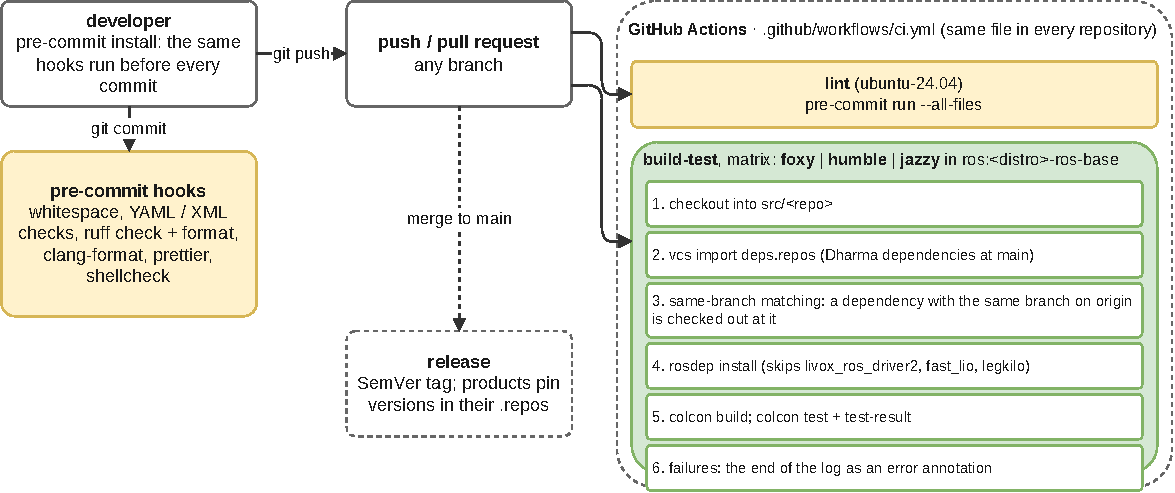
\includegraphics[width=\textwidth]{ci}
  \caption{CI of every Dharma repository: lint, then build and test on Humble and Jazzy with the
    Dharma dependencies on the same branch when it exists.}
  \label{fig:ci}
\end{figure}

Every repository carries the same \code{.github/workflows/ci.yml} (Fig.~\ref{fig:ci}):
\begin{enumerate}
  \item \textbf{lint} on Ubuntu 24.04: \texttt{pre-commit run --all-files}; the end of the log is
    reported as an error annotation on failure.
  \item \textbf{build-test}, matrix \code{humble} and \code{jazzy} in \code{ros:<distro>-ros-base}
    (Python 3.10 with numpy 1.21, and Python 3.12 with numpy 1.26):
    \begin{enumerate}
      \item check out the repository into \code{src/<repo>};
      \item \texttt{vcs import} the Dharma dependencies from \code{deps.repos} (at \code{main});
      \item \textbf{same-branch matching}: every dependency that has the branch under test on
        its origin is checked out at that branch, so a change spanning several repositories is
        built and tested together before it is merged;
      \item \texttt{rosdep install} (skipping \code{livox_ros_driver2}, \code{fast_lio},
        \code{legkilo}, which are built from source on robots);
      \item \texttt{colcon build}, then \texttt{colcon test} of the repository's packages and
        \texttt{colcon test-result}.
    \end{enumerate}
\end{enumerate}
Discovery is limited to localhost in CI (\code{ROS_LOCALHOST_ONLY}, \code{ROS_AUTOMATIC_DISCOVERY_RANGE}).

\section{Releases}

\begin{itemize}
  \item SemVer; before 1.0 a breaking change bumps the minor version and every package of the stack
    moves with it (0.1 $\to$ 0.2). \code{dharma_utils} is a dependency of every package: its API is
    deprecated one minor release before anything is removed.
  \item \code{CHANGELOG.md} in Keep a Changelog format (Added, Changed, Fixed, Removed);
    \code{package.xml} carries the version.
  \item Conventional commits, one short line each (\texttt{fix(mux): rotation inside the field}).
  \item Products pin released versions in their \code{.repos} file (vcstool).
\end{itemize}

\section{The template repository}

The \code{Dharma} repository is the hub of the stack and a GitHub template. It holds
\code{dharma.repos} (every Dharma repository at \code{main}), \code{external.repos}
(\code{livox_ros_driver2}, FAST-LIO, optionally the Leg-KILO fork), a Docker development
environment for Humble and Jazzy (desktop over VNC and noVNC), \code{scripts/dev.sh} and
\code{scripts/setup.sh}, the canonical tooling files, the placeholder bringup package
\code{robot_bringup} (robot profile, stack overrides, \code{robot.launch.py} composing the package
launch files, \code{sim.launch.py} with the simulator) and this documentation. A new product is
created with ``Use this template'' and \texttt{scripts/init\_project.py --name <Repo> --package
<bringup> --robot-ns <ns>}. \todo{verify against the finished template repository (phase 2)}

\section{Building this documentation}

\begin{lstlisting}
make -C docs              # diagrams (when draw.io is installed), manual, paper
make -C docs diagrams     # diagrams/*.drawio -> diagrams/pdf (cropped), diagrams/svg
make -C docs manual       # build/manual/dharma_manual.pdf
make -C docs paper        # build/paper/dharma.pdf
make -C docs reference SRC=~/ws/src   # regenerate manual/generated from the sources
\end{lstlisting}
Diagrams are draw.io files (Helvetica; colours per layer: estimation orange \texttt{\#ffe6cc} /
\texttt{\#d79b00}, world model blue \texttt{\#dae8fc} / \texttt{\#6c8ebf}, planning and execution green
\texttt{\#d5e8d4} / \texttt{\#82b366}, safety red \texttt{\#f8cecc} / \texttt{\#b85450}, utilities yellow
\texttt{\#fff2cc} / \texttt{\#d6b656}, hardware grey \texttt{\#f5f5f5} / \texttt{\#666666}). Their PDF and SVG
exports are committed, so LaTeX builds without draw.io.


\appendix
\chapter{Traceability: findings, fixes and tests}
\label{app:trace}

Every finding of the two reviews of the 0.1 stack, the change that fixes it in 0.2.0 and the
regression tests that cover it. IDs with letters (O1, L1, \ldots) come from the first review (the
mathematical analysis); \code{\#}$n$ IDs come from the second review, numbered per repository.
Priorities: P0 safety, P1 robustness, P2 maintainability (first review). Tests are
\code{file::function} in the package's \code{test/} directory (u: \code{test/unit}, r:
\code{test/ros}); the C++ panels of \pkg{dharma_rviz} have gtests, written
\code{file::Suite.Test} (g: \code{test/}). A cell that says ``no dedicated test'' marks a fix that
is verified only by review or indirectly.

\section{dharma\_odometry}

\begin{small}
\begin{longtable}{@{}>{\raggedright}p{0.07\textwidth}>{\raggedright}p{0.26\textwidth}>{\raggedright}p{0.26\textwidth}>{\raggedright\arraybackslash}p{0.32\textwidth}@{}}
\toprule
  ID & Finding & Fix & Tests \\
  \midrule
  \endhead
  \bottomrule
  \endfoot
  O1 (P1) & the start gate let the estimator start up to 8° tilted, tilting odom and map &
    \param{max_tilt_deg} 3.0 (\code{core/config.py}); Leg-KILO \texttt{init\_type: 2}
    (\code{config/leg_kilo.yaml}); tilt of odom while still in \code{OdometryStatus}
    (\code{core/monitor.py}); levelling in localization &
    u/\code{test_still::test_default_start_tilt_limit_is_three_degrees},
    u/\code{test_still::test_gate_holds_a_tilted_start},
    u/\code{test_monitor::test_level_body_in_a_tilted_odom_is_degraded},
    u/\code{test_monitor::test_tilted_body_in_a_level_odom_is_ok} \\
  O1 & monitor thresholds per robot speed, not a statistical test & residual $\chi^2$ with sensor
    variances and CUSUM (\code{core/residual.py}) &
    u/\code{test_residual::test_lasting_mismatch_alarms_after_a_while_and_recovers},
    u/\code{test_residual::test_threshold_scales_with_the_variances},
    u/\code{test_residual::test_agreeing_speeds_never_alarm_with_sensor_noise} \\
  \#7 & false restart when turning in place near the start pose & a restart needs a message gap
    or a translation jump to the origin, never yaw alone (\code{core/restart.py}) &
    u/\code{test_restart::test_turn_in_place_near_the_start_is_no_restart},
    u/\code{test_restart::test_yaw_snap_alone_is_no_restart},
    r/\code{test_monitor_node::test_turn_in_place_at_the_start_is_no_restart} \\
  \#8 & \texttt{extrinsic\_est\_en: true} for the factory-calibrated Mid-360 IMU & false
    (\code{config/fast_lio.yaml}) &
    r/\code{test_launch::test_fast_lio_does_not_estimate_the_factory_extrinsic} \\
  \#17 & a mistyped \code{site_config} silently ignored & a set but missing file fails the launch &
    r/\code{test_launch::test_missing_site_config_fails_the_launch} \\
  \#3, \#15 & route recorder in odometry (records while not localized, non-atomic CSV) & moved to
    \pkg{dharma_mapping} and fixed there & see dharma\_mapping, recorder \\
  H1 & status as a string & \code{OdometryStatus} (typed) &
    r/\code{test_monitor_node::test_status_is_typed_and_restart_needs_gap_and_origin} \\
  -- & layer inversion: odometry launched localization & include and \code{exec_depend} removed &
    r/\code{test_launch::test_external_starts_only_the_monitor} \\
  -- & empty launch arguments override parameter files & only non-empty arguments override &
    r/\code{test_launch::test_empty_arguments_never_override},
    r/\code{test_launch::test_parameter_files_in_order} \\
\end{longtable}
\end{small}

\section{dharma\_localization}

\begin{small}
\begin{longtable}{@{}>{\raggedright}p{0.07\textwidth}>{\raggedright}p{0.26\textwidth}>{\raggedright}p{0.26\textwidth}>{\raggedright\arraybackslash}p{0.32\textwidth}@{}}
\toprule
  ID & Finding & Fix & Tests \\
  \midrule
  \endhead
  \bottomrule
  \endfoot
  L1 (P1) & one tag detection hard-replaced map$\to$odom: no covariance, no continuous
    correction, ad-hoc 0.5~m / 15° rejection & SE(2) EKF over map$\to$odom with a chi-square gate
    (\code{core/estimator.py}), sources (\code{core/sources/}), optional scan matching,
    \topic{localization/pose} with covariance &
    u/\code{test_estimator::test_predict_grows_with_distance_not_time},
    u/\code{test_estimator::test_gate_grows_with_uncertainty},
    u/\code{test_localizer::test_tag_in_view_localizes_then_corrects_through_the_gate},
    u/\code{test_scan_match::test_match_recovers_the_pose_and_reports_a_covariance} \\
  L2 (P2) & \code{record_tags} slept 2~s in a service callback and blocked the map$\to$odom
    timer & timer-driven recording session, own callback group (\code{core/tags.py},
    \code{utils/tag_services.py}) &
    r/\code{test_localization_node::test_record_tags_keeps_tf_flowing_and_relocalizes} \\
  O1 (P1) & odom not level & levelling in the bridge (\code{core/leveling.py},
    \code{core/bridge.py}) &
    u/\code{test_leveling_bridge::test_level_rotation_removes_the_start_tilt_of_the_base},
    u/\code{test_leveling_bridge::test_level_bridge_keeps_lio_motion_planar_on_a_tilted_start},
    r/\code{test_localization_node::test_bridge_levels_odom_and_reset_clears} \\
  T1/T3, \#14 & tf2 interpolated a ramp across a correction & old value at $t - \epsilon$, new
    at $t$ (\code{core/timeline.py}) &
    u/\code{test_leveling_bridge::test_timeline_steps_within_epsilon_never_ramps},
    u/\code{test_localizer::test_correction_samples_step_without_ramp} \\
  \#1 & auto-correct gate compared map$\to$odom instead of map$\to$base & innovation on the robot
    pose & u/\code{test_estimator::test_gate_rejects_outliers_and_accepts_consistent_fixes_far_from_origin},
    u/\code{test_estimator::test_heading_uncertainty_far_from_origin_moves_the_robot_sideways} \\
  \#2 & \code{record_tags} allowed while not localized, overwriting the site anchors & refuse
    unless \code{LOCALIZED} and not circular &
    u/\code{test_tags::test_recordable_refuses_when_not_localized_or_circular},
    u/\code{test_localizer::test_record_refused_when_not_localized_and_when_circular} \\
  \#3 & a corrupt tags file crashed \code{record_tags} & tolerant reads, \texttt{success: false} &
    u/\code{test_tags::test_merge_refuses_to_overwrite_a_corrupt_file},
    u/\code{test_localizer::test_record_session_writes_the_tag_and_survives_a_corrupt_file} \\
  \#10 & an empty launch argument overrode the params file & non-empty overrides only &
    u/\code{test_launch::test_empty_arguments_do_not_override} \\
  \#11 & \code{~} in the tags file not expanded & \code{dharma_utils.io.expand} &
    r/\code{test_localization_node::test_tags_file_with_tilde_is_expanded} \\
  \#12 & \code{load_tags} wrote anywhere & path must resolve inside \param{sites_dir} &
    r/\code{test_localization_node::test_load_tags_path_guard_and_corrupt_file} \\
  \#15 & tag tests without the real optical rotation & tests with $(-\pi/2, 0, -\pi/2)$ and
    non-zero yaws, hand-computed poses &
    u/\code{test_tag_geometry::test_optical_rotation_is_right_down_forward},
    u/\code{test_tag_geometry::test_tag_off_axis_and_rotated_robot_yawed_90_degrees} \\
\end{longtable}
\end{small}

\section{dharma\_perception}

\begin{small}
\begin{longtable}{@{}>{\raggedright}p{0.07\textwidth}>{\raggedright}p{0.26\textwidth}>{\raggedright}p{0.26\textwidth}>{\raggedright\arraybackslash}p{0.32\textwidth}@{}}
\toprule
  ID & Finding & Fix & Tests \\
  \midrule
  \endhead
  \bottomrule
  \endfoot
  P1 (P1) & height band in base\_link, which pitches with the gait; base height 0.35 here and
    0.30 elsewhere & levelled points, band above the floor from \param{robot.base_height},
    optional ground segmentation (\code{core/filtering.py}) &
    u/\code{test_filtering::test_pitched_body_does_not_see_the_floor},
    u/\code{test_filtering::test_band_is_relative_to_the_floor_through_base_height},
    r/\code{test_lidar_sector_node::test_pitched_body_does_not_block_on_the_floor} \\
  P1 & minimum of one point per sector sensitive to outliers & $k$-th nearest point
    (\code{core/sectors.py}) &
    u/\code{test_sectors::test_kth_nearest_ignores_a_single_spurious_return} \\
  P2 (P1) & visitor tracker associated in a rotating frame & removed (product feature) & -- \\
  B4 & low objects near the robot drop out of view; sectors without returns read free &
    obstacle memory in odom (\code{core/memory.py}); limits documented &
    u/\code{test_memory_blindness::test_memory_keeps_an_object_the_sensor_no_longer_sees},
    u/\code{test_pipeline::test_memory_keeps_a_low_box_in_the_safety_scan} \\
  -- & blind sensor not reported & every sector \code{BLOCKED} when blind, TF missing, errors or
    silence (\code{core/blindness.py}, node watchdog) &
    u/\code{test_pipeline::test_blind_lidar_blocks_every_sector},
    r/\code{test_lidar_sector_node::test_blind_livox_blocks_every_sector},
    r/\code{test_lidar_sector_node::test_silent_input_publishes_blocked_scans} \\
  \#4 & one malformed cloud killed the producer & validated parsing, per-message try/except,
    respawn & u/\code{test_livox::test_fuzz_never_raises_anything_else},
    r/\code{test_lidar_sector_node::test_malformed_livox_bytes_keep_the_node_alive},
    r/\code{test_lidar_sector_node::test_pointcloud_input_and_malformed_clouds} \\
  \#12 & Livox tag bits ignored & noise filter per field and confidence &
    u/\code{test_livox::test_noise_mask_selects_fields_and_levels},
    r/\code{test_lidar_sector_node::test_livox_noise_tags_are_dropped} \\
  \#16 & the Livox path had no real test & raw-bytes node test, packer checked against the
    documented layout & r/\code{test_lidar_sector_node::test_livox_raw_bytes_give_front_and_safety_scans},
    u/\code{test_livox::test_packer_matches_the_documented_layout} \\
\end{longtable}
\end{small}

\section{dharma\_mapping}

\begin{small}
\begin{longtable}{@{}>{\raggedright}p{0.07\textwidth}>{\raggedright}p{0.26\textwidth}>{\raggedright}p{0.26\textwidth}>{\raggedright\arraybackslash}p{0.32\textwidth}@{}}
\toprule
  ID & Finding & Fix & Tests \\
  \midrule
  \endhead
  \bottomrule
  \endfoot
  M1 (P1) & scans integrated at the TF pose without any check & jump and correction gates,
    optional refinement (\code{core/integrator.py}); pose graph future work &
    u/\code{test_integrator::test_jump_is_rejected_and_never_grows_the_grid},
    u/\code{test_integrator::test_refinement_keeps_walls_sharp_under_pose_error},
    u/\code{test_integrator::test_refinement_refuses_an_ambiguous_corridor} \\
  O1 & band assumed a level map frame without saying so & band in the levelled map frame,
    documented & u/\code{test_integrator::test_band_drops_floor_ceiling_and_the_robot} \\
  I1, §5.4 & site manager mixed map storage with POIs and tours & POIs and tours removed & -- \\
  \#4 & \code{mapping/save} wrote another site's grid; a timed-out stop counted as stopped & the
    session remembers its site (\code{core/session.py}); a timeout is a failure &
    u/\code{test_session::test_session_refuses_to_save_another_sites_grid},
    r/\code{test_site_manager_node::test_timed_out_stop_is_a_failure} \\
  \#5 & no \code{.bak}, map pair not atomic, reset of the same site skipped the archive & atomic
    pair with size and CRC, \code{.bak} pair (\code{core/map_io.py}); reset always archives &
    u/\code{test_map_io::test_previous_pair_is_kept_as_a_loadable_backup},
    u/\code{test_map_io::test_torn_pair_is_detected},
    u/\code{test_map_io::test_failed_write_leaves_the_old_pair},
    u/\code{test_session::test_reset_always_archives_existing_content} \\
  \#7 & corrupt site files crashed the site manager at every boot & tolerant loads, notes in
    \topic{site/status} (\code{core/site_store.py}) &
    u/\code{test_site_store::test_corrupt_files_never_raise},
    r/\code{test_site_manager_node::test_corrupt_site_files_do_not_crash_the_boot} \\
  \#8 & unbounded grid growth on odometry jumps (300~m: 109~MB) & size cap and jump gate
    (\code{core/grid.py}) & u/\code{test_grid::test_growth_is_capped_on_a_pose_jump},
    u/\code{test_grid::test_cap_splits_the_room_when_both_sides_grow} \\
  \#9 & an \code{origin} localization at boot trusted as the frame of an existing site & only
    tag or pose-estimate localization continues a site &
    u/\code{test_session::test_origin_at_boot_is_not_the_frame_of_an_existing_site},
    r/\code{test_site_manager_node::test_origin_at_boot_does_not_continue_an_existing_site} \\
  \#10 & launch defaults overrode the params file & non-empty overrides only &
    r/\code{test_launch::test_empty_arguments_add_no_overrides},
    r/\code{test_launch::test_missing_params_file_fails_the_launch} \\
  \#11 & \code{~} not expanded (recorder output, tags path) & \code{dharma_utils.io.expand} &
    u/\code{test_routes::test_output_path_is_expanded_and_empty_refuses} \\
  \#12 & \code{grid_mapper/save|load} accepted any path & site names only &
    r/\code{test_grid_mapper_node::test_scans_become_a_grid_saved_into_its_own_site},
    r/\code{test_grid_mapper_node::test_continue_needs_the_site_loaded} \\
  \#13 & archives collided within a second, nested routes, were made before the preconditions &
    \code{unique_dir}, preconditions first &
    u/\code{test_site_store::test_archive_twice_in_one_second_never_nests},
    r/\code{test_site_manager_node::test_reset_archives_into_unique_directories},
    r/\code{test_site_manager_node::test_reset_archives_only_when_it_can_start} \\
  \#14 & scans integrated during a map$\to$odom correction & correction gate &
    u/\code{test_integrator::test_scans_during_a_correction_are_skipped} \\
  rec. & recorder recorded while not localized (TF exists $\ne$ localized) & only while
    \code{LOCALIZED} (\code{core/routes.py}) &
    u/\code{test_routes::test_refuses_when_not_localized},
    r/\code{test_route_recorder_node::test_refuses_while_not_localized_even_with_tf} \\
  rec. & non-atomic, all-in-memory CSV & incremental atomic writes &
    u/\code{test_routes::test_route_goes_to_the_site_and_is_written_incrementally} \\
  rec. & an \code{OSError} in the service killed the node & \texttt{success: false} &
    r/\code{test_route_recorder_node::test_file_errors_are_answers_not_crashes} \\
\end{longtable}
\end{small}

\section{dharma\_navigation}

\begin{small}
\begin{longtable}{@{}>{\raggedright}p{0.07\textwidth}>{\raggedright}p{0.26\textwidth}>{\raggedright}p{0.26\textwidth}>{\raggedright\arraybackslash}p{0.32\textwidth}@{}}
\toprule
  ID & Finding & Fix & Tests \\
  \midrule
  \endhead
  \bottomrule
  \endfoot
  N1 (P0) & planner radius 0.35~m below the half diagonal 0.49~m & lethal = inscribed radius +
    margin, oriented footprint check up to the circumscribed radius
    (\code{core/planning/costmap.py}, \code{footprint.py}) &
    u/\code{test_planning::test_radii_come_from_the_footprint},
    u/\code{test_planning::test_oriented_footprint_against_a_wall},
    u/\code{test_planning::test_door_narrower_than_the_body_is_refused} \\
  N2 (P2) & MPPI without obstacle cost, warm start or seed; PID without anti-windup;
    SpeedRegulator integrating $|\omega|$ & obstacle cost, warm start, seeded RNG
    (\code{core/controllers/mppi.py}); clamped integral (\code{pid.py}); signed error, reset on
    new paths & u/\code{test_controllers::test_mppi_is_seeded_and_warm_started},
    u/\code{test_controllers::test_mppi_steers_around_scan_obstacles},
    u/\code{test_controllers::test_pid_integral_is_clamped_and_recovers};
    regulator: no dedicated test \\
  N3 (P1) & two stopping models (path shift without reaction time) & \code{dharma_utils.safety}
    for path shift, profile and guard & u/\code{test_path::test_profile_brakes_into_stops_with_the_stopping_model},
    u/\code{test_shift::test_no_gap_slows_to_a_stop_with_the_stopping_model} \\
  N4 (P0) & \code{steering_bias} a rate in the message, an angle in one controller &
    \code{heading_offset} (rad) and \code{yaw_rate_bias} (rad/s) in every controller &
    u/\code{test_controllers::test_biases_have_one_meaning_in_every_controller} \\
  N5 (P2) & hard-coded \code{'map'} / \code{'base_link'} & \param{robot.frames} & no dedicated
    test: the node tests run with the default frames; no frame literal is left in the package
    sources \\
  -- & speed profile without a forward pass & forward pass (\code{core/path/profile.py}) &
    u/\code{test_path::test_profile_forward_pass_limits_acceleration} \\
  §4 & stale TF stopped the robot without distinction & ages from \code{self.tf}, prediction
    between \param{tf_compensate_sec} and the timeout, \code{TF_STARTING} / \code{TF_STALE} /
    \code{TF_CLOCK} (\code{core/follower/supervisor.py}) &
    u/\code{test_follower_safety::test_tf_status_messages},
    u/\code{test_follower_safety::test_slightly_old_pose_is_predicted_with_the_twist} \\
  -- & \code{path_follower_node} 1429 lines & pure follower in \code{core/follower/}, node 277
    lines & \code{test_style::test_package_conventions} \\
  F1 & blind scan (0 / NaN sectors) read as clear in path shift and planner & blocked = stop &
    u/\code{test_shift::test_blind_scan_stops},
    r/\code{test_planner_node::test_blocked_replans_and_blind_scan_fails},
    u/\code{test_avoidance::test_blind_sectors_ahead_stop_the_robot},
    r/\code{test_obstacle_avoidance_node::test_blind_scan_is_an_emergency} \\
  F2 & a stop could leave a moving command last; no zero on shutdown & zero on entering
    INACTIVE, shutdown hook, state lock &
    u/\code{test_follower::test_stop_zeroes_once_and_start_resumes},
    r/\code{test_path_follower_node::test_follow_pause_estop_resume_and_shutdown} \\
  F3 & start raced the control tick & one mutually exclusive group for state changes and the
    control loop, asynchronous hook calls &
    r/\code{test_path_follower_node::test_follow_pause_estop_resume_and_shutdown} \\
  F4 & path-shift speed limit from the commanded offset only & also the measured offset &
    u/\code{test_shift::test_measured_offset_limits_the_speed} \\
  F5 & progress jumped to a parallel leg while shifted & windowed, offset-compensated
    projection, capped advance (\code{core/path/progress.py}) &
    u/\code{test_path::test_shifted_progress_stays_on_its_leg},
    u/\code{test_follower::test_overlapping_legs_keep_progress_and_stops} \\
  F6 & stop points skipped while shifted or triggered early from another leg & detection by
    progress and distance minus offset; wait at a stop with an obstacle &
    u/\code{test_follower::test_overlapping_legs_keep_progress_and_stops},
    u/\code{test_follower::test_stop_point_with_an_obstacle_waits_instead_of_passing} \\
  F7 & joining and final approach checked by the front cone only; timers ran while paused &
    360° motion guard in every phase; timers frozen &
    u/\code{test_follower_safety::test_joining_is_guarded_by_the_scan},
    u/\code{test_follower::test_dwell_timer_is_frozen_while_paused} \\
  F8 & snapped goals never arrived & arrival against the plan goal &
    u/\code{test_session::test_arrival_is_tested_against_the_snapped_goal},
    r/\code{test_planner_node::test_go_to_arrives_on_the_plan_goal_and_stops} \\
  F9 & planner failed but the follower kept going & stop on every failure after \code{set_path}
    & u/\code{test_session::test_follower_failure_stops_and_fails},
    u/\code{test_session::test_blocked_replans_then_gives_up_and_stops} \\
  F10 & cancel blocked behind planning & own callback group, cancel flag &
    r/\code{test_planner_node::test_cancel_is_not_blocked_by_a_slow_send} \\
  F11 & numeric parameters unchecked (NaN, zero temperature, negative accelerations) & typed
    configuration with ranges, NaN $\to$ 0 & u/\code{test_follower_safety::test_config_ranges_and_cross_checks},
    u/\code{test_follower_safety::test_shaper_envelope_slew_and_nan},
    r/\code{test_path_follower_node::test_invalid_parameters_are_rejected} \\
  F12 & route processing dropped stop points closer than 3~cm & anchors kept &
    u/\code{test_path::test_close_stop_points_are_all_kept} \\
  F13 & avoidance smoothing slowed braking & asymmetric smoothing &
    u/\code{test_avoidance::test_smoothing_never_slows_braking},
    u/\code{test_avoidance::test_policy_brakes_in_one_scan_with_heavy_smoothing} \\
  F14, B2 & default \code{cmd_vel} bypassed the mux & \topic{control/nav_cmd_vel} (fixed
    name, \code{utils/outputs.py}) &
    r/\code{test_path_follower_node::test_follow_pause_estop_resume_and_shutdown} \\
  F15 & path shift kept after a mode change; costmap cache not invalidated; planner pose without
    TF age check & reset on mode change, rebuild on parameter change, age check &
    u/\code{test_follower::test_mode_change_drops_the_path_shift},
    r/\code{test_planner_node::test_go_to_arrives_on_the_plan_goal_and_stops} (costmap dropped on
    a parameter change); planner pose age (\code{tf.fresh} with \param{tf_timeout_sec}): no
    dedicated test \\
  F16 & ``paused until relocalized'' never un-paused & pause reasons (\code{core/follower/pause.py})
    & u/\code{test_follower_safety::test_relocalization_unpauses},
    u/\code{test_follower_safety::test_estop_is_sticky_and_remote_is_transient} \\
  F17 & one-point path accepted; pending inspections survived a restart; route markers keyed on
    the count; line of sight through diagonal pinches & two points required; inspection rounds;
    markers by route; corner cells counted & u/\code{test_path::test_route_needs_two_points_and_length},
    u/\code{test_follower::test_late_inspection_answers_are_dropped_after_a_restart},
    u/\code{test_planning::test_line_of_sight_blocks_diagonal_pinches} \\
  F18 & missing tests (transitions, zero on stop / e-stop / stale / pause / shutdown, path shift
    lag, blind scans, overlapping legs) & added & u/\code{test_follower::test_transition_table},
    u/\code{test_follower_safety::test_every_hold_publishes_zero_every_tick} and the tests above \\
\end{longtable}
\end{small}

\section{dharma\_control}

\begin{small}
\begin{longtable}{@{}>{\raggedright}p{0.07\textwidth}>{\raggedright}p{0.26\textwidth}>{\raggedright}p{0.26\textwidth}>{\raggedright\arraybackslash}p{0.32\textwidth}@{}}
\toprule
  ID & Finding & Fix & Tests \\
  \midrule
  \endhead
  \bottomrule
  \endfoot
  C1 (P0) & rotation not limited by the field & rotation room and combined-motion arc
    (\code{core/field.py}, \code{core/arc.py}) &
    u/\code{test_field::test_rotation_next_to_an_obstacle_is_limited},
    u/\code{test_field::test_rotation_limit_follows_the_yaw_stopping_model},
    u/\code{test_field::test_combined_motion_checks_the_arc},
    r/\code{test_control_mux_node::test_field_limits_rotation_beside_an_obstacle} \\
  C2 (P0) & software-only safety & \topic{control/hw_estop}, two-channel architecture documented
    (README, Section~\ref{sec:two-channel}) &
    u/\code{test_arbiter::test_hardware_estop_engages_and_blocks_release},
    u/\code{test_arbiter::test_silent_hardware_estop_engages_when_required} \\
  N3 & own stopping model & \code{dharma_utils.safety} only &
    u/\code{test_field::test_wall_ahead_limits_with_the_shared_stopping_model} \\
  -- & field off in REMOTE by default & \param{field.in_remote} true with its own margin &
    r/\code{test_control_mux_node::test_field_on_in_remote_by_default},
    u/\code{test_field::test_remote_uses_its_margin_and_can_be_switched_off} \\
  B1 & blind LiDAR (all sectors 0) read as clear & blocked sectors are obstacles, BLIND $\to$
    zero & u/\code{test_scan::test_all_sectors_zero_is_blind_not_clear},
    u/\code{test_field::test_blind_scan_stops_auto},
    r/\code{test_control_mux_node::test_blind_scan_stops_auto_and_creeps_remote} \\
  B3 & e-stop resumed through \code{set_mode}; fire-and-forget pause calls; release forwarded
    the held stick command & no navigation calls; re-arm with neutral commands
    (\code{core/arbiter.py}) &
    u/\code{test_arbiter::test_release_requires_rearm_and_never_forwards_the_held_command},
    u/\code{test_arbiter::test_switch_to_remote_ignores_a_stick_held_during_the_switch} \\
  \#3 & SetBool default request released the e-stop; anyone released anyone's & Trigger engage
    and release &
    r/\code{test_control_mux_node::test_estop_service_holds_zero_and_release_needs_rearm} \\
  \#4 & watchdog and hold on the ROS clock & steady clock &
    r/\code{test_control_mux_node::test_watchdog_and_hold_run_on_steady_time_with_sim_time} \\
  \#5 & parameters ignored at runtime; \texttt{max\_decel: 0} crashed; NaN limits disabled the
    envelope & read-only validated parameters; non-finite $\to$ zero &
    u/\code{test_arbiter::test_config_validation},
    r/\code{test_control_mux_node::test_bad_values_refuse_to_start},
    u/\code{test_envelope::test_non_finite_on_any_axis_is_zero} \\
  \#6 & no zero on shutdown or crash & shutdown hook, e-stop on callback errors &
    r/\code{test_control_mux_node::test_shutdown_hook_publishes_zeros},
    r/\code{test_control_mux_node::test_callback_error_engages_the_estop} \\
  \#7 & scan freshness by receive time only; NaN sectors free; frame and coverage unchecked &
    scan validation (\code{core/scan.py}) & u/\code{test_scan::test_header_age_old_and_future},
    u/\code{test_scan::test_wrong_frame_is_rejected},
    u/\code{test_scan::test_partial_coverage_is_rejected},
    u/\code{test_scan::test_blocked_or_unknown_sectors_are_blind} \\
  \#8 & several remote operators on one topic & one topic per source &
    u/\code{test_arbiter::test_only_the_active_source_is_forwarded},
    r/\code{test_control_mux_node::test_remote_sources_and_set_mode} \\
  \#13 & re-sending the same mode injected a zero & no-op &
    u/\code{test_arbiter::test_set_mode_same_mode_and_source_is_a_no_op} \\
  \#14 & a second e-stop reason overwrote the first without republish & reasons accumulate,
    status republished & u/\code{test_arbiter::test_estop_reasons_are_kept_oldest_first_without_duplicates},
    r/\code{test_control_mux_node::test_estop_request_topic_appends_reasons} \\
\end{longtable}
\end{small}

\section{dharma\_health}

\begin{small}
\begin{longtable}{@{}>{\raggedright}p{0.07\textwidth}>{\raggedright}p{0.26\textwidth}>{\raggedright}p{0.26\textwidth}>{\raggedright\arraybackslash}p{0.32\textwidth}@{}}
\toprule
  ID & Finding & Fix & Tests \\
  \midrule
  \endhead
  \bottomrule
  \endfoot
  H1 (P2) & status as JSON in \code{std_msgs/String}, not actionable & \code{HealthStatus} +
    \code{DiagnosticArray}, \code{speed_scale} for the mux &
    u/\code{test_report::test_lidar_rate_low_or_tf_late_halves_the_speed},
    u/\code{test_report::test_error_stops_and_comes_first},
    u/\code{test_report::test_lowest_matching_rule_wins_and_rules_never_raise_an_error},
    r/\code{test_health_node::test_core_states_match_the_messages} \\
  -- & rates only: a 10~Hz topic with 2~s old stamps passed & header stamp age per topic,
    negative ages; raw subscription, stamp read from the CDR bytes &
    u/\code{test_sensors::test_10hz_topic_with_2s_old_stamps_warns},
    u/\code{test_sensors::test_stamps_from_the_future_are_a_clock_offset},
    u/\code{test_sensors::test_slow_and_silent_topics},
    u/\code{test_sensors::test_cdr_stamp_both_byte_orders},
    r/\code{test_health_node::test_stamp_from_a_real_serialized_message} \\
  T1--T5 & TF staleness without diagnosis & per-edge ages classified as clock offset or load;
    optional chrony check & u/\code{test_tf::test_steady_late_edge_is_a_clock_offset},
    u/\code{test_tf::test_growing_ages_are_load}, u/\code{test_tf::test_stopped_publisher},
    u/\code{test_tf::test_future_stamps_and_few_samples},
    u/\code{test_tf::test_clock_check_runs_the_command_once_per_period},
    r/\code{test_health_node::test_tf_edge_with_a_steady_offset_is_a_clock_problem} \\
  \#9 & health OK while not localized & \code{NONE} is a warning &
    u/\code{test_state::test_not_localized_is_a_warning},
    r/\code{test_health_node::test_old_stamps_not_localized_then_ok_then_lost} \\
  -- & safety scan and control field not watched & \code{state:safety_scan} and
    \code{state:control} (stale or blind is an error) & u/\code{test_state::test_safety_scan},
    u/\code{test_state::test_control_states},
    r/\code{test_health_node::test_blind_safety_scan_is_an_error} \\
  \#13 & missing-node check ignored namespaces & fully qualified names &
    u/\code{test_state::test_nodes_with_namespaces},
    r/\code{test_health_node::test_expected_node_in_another_namespace_is_missing} \\
  \#17 & unreadable thermal zone or disk reported OK & ``unreadable'' warning, thermal zone
    whitelist & u/\code{test_system::test_unreadable_values_warn},
    u/\code{test_system::test_whitelisted_zones_only},
    u/\code{test_system::test_no_whitelisted_zone_warns} \\
\end{longtable}
\end{small}

\section{dharma\_sim}

\begin{small}
\begin{longtable}{@{}>{\raggedright}p{0.07\textwidth}>{\raggedright}p{0.26\textwidth}>{\raggedright}p{0.26\textwidth}>{\raggedright\arraybackslash}p{0.32\textwidth}@{}}
\toprule
  ID & Finding & Fix & Tests \\
  \midrule
  \endhead
  \bottomrule
  \endfoot
  S1 (P2) & perfect odometry, stamps with \code{now()} & drift model, latency, LiDAR dropout,
    seeded scenarios & u/\code{test_odometry::test_random_walk_grows_with_the_square_root_of_distance},
    u/\code{test_odometry::test_scale_error_and_yaw_bias_accumulate},
    u/\code{test_odometry::test_same_seed_same_run},
    u/\code{test_latency::test_sensor_stamp_is_now_minus_latency},
    u/\code{test_scenario::test_seeded_generators_are_reproducible_and_independent},
    u/\code{test_scenario::test_dropouts_and_restarts},
    r/\code{test_sim_robot_node::test_stamps_carry_the_latency},
    r/\code{test_sim_robot_node::test_scenario_dropout_silences_the_lidar} \\
  \#10 & ray cast blind from inside a circle; no collisions; LiDAR ignored the vertical field of
    view and the minimum range & fixed ray cast, collision latch, Mid-360 model &
    u/\code{test_world::test_ray_from_inside_a_circle_sees_its_far_side},
    u/\code{test_world::test_collisions_with_walls_and_circles},
    u/\code{test_body::test_collision_stops_and_latches},
    u/\code{test_lidar::test_low_obstacle_hidden_below_the_lowest_beam},
    u/\code{test_lidar::test_min_and_max_range},
    r/\code{test_sim_robot_node::test_collision_latches_and_stops} \\
  \#11 & \code{imu_in_lidar} sign (FAST-LIO's $T_{IL}$) & Livox manual values, derived
    consistently & u/\code{test_odometry::test_imu_offset_follows_the_livox_manual},
    u/\code{test_odometry::test_lio_pose_closes_the_bridge_chain} \\
  \#14 & fixed $\Delta t$ per wall-timer tick (time dilation under load) & measured $\Delta t$,
    clamped to \param{max_dt} & u/\code{test_body::test_measured_dt_not_ticks},
    u/\code{test_body::test_stall_is_clamped_to_max_dt} \\
\end{longtable}
\end{small}

\section{dharma\_rviz}

\begin{small}
\begin{longtable}{@{}>{\raggedright}p{0.07\textwidth}>{\raggedright}p{0.26\textwidth}>{\raggedright}p{0.26\textwidth}>{\raggedright\arraybackslash}p{0.32\textwidth}@{}}
\toprule
  ID & Finding & Fix & Tests \\
  \midrule
  \endhead
  \bottomrule
  \endfoot
  \#9 & Tuning: live apply by default, wheel scrolling edits gains, no bounds & apply-on-change
    off, ranges from descriptors, wheel only with focus &
    g/\code{test_tuning::TuningTest.EditorsFollowTheDescriptors},
    g/\code{test_tuning::TuningTest.WheelIgnoredAndEditsWaitForApply} \\
  \#10 & duplicate panels in \code{robot.rviz}; fixed node names per panel & duplicates removed,
    unique node names & g/\code{test_panels::PanelTest.PanelsGetUniqueNodeNames},
    g/\code{test_common::Names.UniqueNodeNamesPerInstance},
    g/\code{test_plugins::Plugins.EveryPanelLoads}; \code{robot.rviz}: no dedicated test \\
  \#11 & no e-stop, mode or field state in RViz; Start resumed during an e-stop & Safety panel;
    Start disabled while \code{ControlStatus.estop} &
    g/\code{test_panels::PanelTest.MissionStartDisabledDuringEstop},
    g/\code{test_panels::PanelTest.SafetyEstopAlwaysEnabled},
    g/\code{test_common::Format.NavigationButtonsFollowStateAndEstop} \\
  \#15 & \code{wait_for_service} blocked the Qt thread; load race; 4 decimals; string arrays
    split on commas & asynchronous readiness, client per request, full precision &
    g/\code{test_panels::PanelTest.ServiceCallTimesOut},
    g/\code{test_panels::PanelTest.ServiceCallReportsUnavailableAndSuccess},
    g/\code{test_tuning::TuningTest.SecondLoadWins},
    g/\code{test_tuning::TuningYaml.ExportKeepsPrecision},
    g/\code{test_common::Yaml.ListLines} \\
  \#16 & Tag panel buttons stuck; only the first diagnostic shown; values never stale &
    timeouts, worst status, age indicator &
    g/\code{test_panels::PanelTest.TagButtonsComeBackAfterTheReply},
    g/\code{test_common::Diagnostics.WorstOfAllFreshStatuses},
    g/\code{test_common::Staleness.GoesStaleAfterTimeout} \\
\end{longtable}
\end{small}

\section{dharma\_interfaces and cross-stack findings}

\begin{small}
\begin{longtable}{@{}>{\raggedright}p{0.07\textwidth}>{\raggedright}p{0.26\textwidth}>{\raggedright}p{0.26\textwidth}>{\raggedright\arraybackslash}p{0.32\textwidth}@{}}
\toprule
  ID & Finding & Fix & Tests \\
  \midrule
  \endhead
  \bottomrule
  \endfoot
  I1 (P2) & core and application (tour guide) types mixed & POI, tour, visitor and mission types
    removed; products own them & -- \\
  N4 & \code{AvoidanceCommand.steering_bias} unit ambiguous & \code{heading_offset} (rad),
    \code{yaw_rate_bias} (rad/s) & see dharma\_navigation N4 \\
  H1 & status as strings everywhere & typed status messages with enum constants & package tests
    of every publisher \\
  P2 (§5.3) & duplication: 15 \code{main()} boilerplates, 11 latched QoS definitions, 5 yaw
    implementations, 7 identical \code{test_node_members.py} & \pkg{dharma_utils}
    (\code{run}, QoS, math, \code{check_package}) & \pkg{dharma_utils} unit tests;
    \code{test_style} in every package \\
  §5.2 & robot description in about six files & \code{RobotProfile} shared through
    \param{robot.*} & u/\code{test_config::test_robot_profile_derived_values} (dharma\_utils) \\
\end{longtable}
\end{small}


\bibliographystyle{IEEEtran}
\bibliography{references}

\end{document}
